% Remove the oneside option below for double sided printing (e.g. for final (post-viva) submission)
\documentclass[a4paper,12pt,oneside,openright]{book}

% Preamble commands go here
\renewcommand{\labelenumi}{\theenumi}
\usepackage{customisations}
\usepackage{rotating}

%% Some of the below packages may be useful to thesis writers in Physics
%% Googling `latex <packagename>' will usually give you some documentation
% \usepackage[load-configurations=abbreviations]{siunitx} % siunitx typesets physical units in a consistent manner
\usepackage{booktabs} % booktabs provides professional formatting commands for tables
\usepackage{amsmath} % amsmath provides extra maths symbols

\usepackage{textcomp} % textcomp provides extra text symbols (like a degrees celsius symbol)
\usepackage[flushleft]{threeparttable}
% \usepackage{tikz} % tikz is a package for drawing diagrams and adding annotations to figures
% \usepackage{threeparttable} % threeparttable allows for adding notes to tables
% \usepackage{eps2pdf} % eps2pdf allows background transformation of eps files to pdfs so they
%						work seamlessly with pdflatex. If using this with the LaTeX editor Kile,
%						you need to add --shell-escape before '%source', in
%						Settings -> Configure Kile... -> Tools -> Build -> build_pdflatex

% End preamble

% REPLACE THESE with your thesis title, your name and the date of submission of the thesis
\title{Red Supergiant Stars within the Local Group}
\author{Lee. R. Patrick}
\date{March 2016} % of submission

\begin{document}


% Thesis front matter - title page, abstract, acknowledgements, declaration and table of contents
% See customisations.sty to modify the title page or declaration
\singlespacing
\maketitlepage
\frontmatter
\eighteenptleading
%%%%%%%%%%%%%%%%%%%%%%%%%%%%%%%%%%%%%%%%%%%%%%%%%%%%%%%%%%%%%%%%%%%%%%%%%%%%%%
% Re include for the final thing!

% \chapter{Abstract}

Red Supergiant (RSG) stars are the most luminous stars in the infrared sky.
Their intrinsic luminosities combined with the low dust extinction observed
in this regime makes these objects very attractive to study in the near-infrared (IR).
In addition, RSGs are necessarily young objects,
as, they are tracers of recent star formation in extra-galactic
systems.
As the next generation of telescopes will be optimised for study in the near-IR,
it is clear that, in the coming years, RSGs will play a prominent role in the way that astronomers probe the local Universe and out to larger distances with
space-based observations.
Therefore, it is vital to better our understanding of these objects now and develop the
tools that will allow us to take full advantage of the suite of instrumentation
that will become available in the near future.
This thesis aims to further the understanding of RSGs by focusing on quantitative studies of near-IR spectroscopic observations.

To this end, I develop an analysis technique that uses spectroscopic and photometric observations to estimate stellar parameters of RSGs.
The observations are compared with synthetic spectra extracted from stellar model atmospheres, where departures from local thermodynamic equilibrium have been calculated for the diagnostic spectral lines.
This technique is tested thoroughly on synthetic and real observations and is shown to reliably estimate stellar parameters in both regimes when compared with input parameters and previous studies respectively.


Using the analysis routines developed in Chapter~\ref{ch:janal}, in Chapter~\ref{ch:ngc2100} I measure the chemistry and kinematics of NGC\,2100, a young massive cluster (YMC) of stars in the Large Magellanic Cloud, using near-IR spectroscopic observations of 14 RSGs taken with the new $K$-band multi-object spectrograph (KMOS).
I estimate the average metallicity to be $-$0.43\,$\pm$\,0.10\,dex, which is in good agreement with previous studies.
I compare the observed location of the target RSGs on the Hertzsprung--Russell diagram with that of a Solar-like metallicity YMC and show that there appears to be no significant difference in the appearance of the RSGs in these two clusters.
By combining the individual RSG spectra, I create an integrated-light cluster spectrum and show that the stellar parameters estimated, using the same technique as for individual RSGs, are in good agreement with the average properties of the cluster.
In addition, I measure -- for the first time -- an upper limit of the dynamical mass of NGC\,2100 to be 15.2~$\times$~10$^4$\,M$_{\odot}$, which is consistent with the literature measurement of the photometric mass of the cluster.


In Chapter~\ref{ch:ngc6822}, I present observations of RSGs in NGC\,6822, a dwarf irregular with a turbulent history, observed with KMOS.
The data reduction process with KMOS is described in detail, in particular
where the reduction has been optimised for the data.
Stellar parameters are estimated using the technique presented in Chapter~\ref{ch:janal} and an average metallicity in NGC\,6822 of $-$0.55\,$\pm$\,0.13\,dex is found, consistent with previous measurements of young stars in this galaxy.
The spatial distribution of metallicity is estimated and weak evidence is found for a radial metallicity gradient, which will require follow-up observations.
In addition, I show that the metallicities of the young and old populations of NGC\,6822 are well explained using a simple closed-box chemical evolution model, an interesting result, as NGC\,6822 is expected to have undergone significant recent interactions.


In Chapter~\ref{ch:ngc55}, I present multi-epoch KMOS observations of 22 RSGs in the Sculptor Group galaxy NGC\,55.
Radial velocities are measured for the sample and are shown to be in good agreement with previous studies. Using the multi-epoch data, I find no evidence for radial velocity variables within the sample.
Stellar parameters are estimated for 10 targets and are shown to be in good agreement with previous estimates.

I conclude this thesis by summarising the main results and present a first-look calibration of the relationship between galaxy mass and metallicity using RSGs.
By comparing the RSG metallicity estimates to metallicities estimated from $\sim$50\,000 Sloan digital sky survey galaxies, I show that the absolute metallicities of the two samples disagree. A more quantitative analysis requires additional RSG observations.

In addition, using $\sim$80 RSGs, with stellar parameters estimated in a consistent way, I show that there appears to be no dependence of the temperature of RSGs upon metallicity.
This is in disagreement with current evolutionary models, which display a temperature change of $\sim$450\,K over the studied range in metallicity.

Finally, I outline potential areas for future work, focusing on follow-up studies that have been identified as a result of the work done in this thesis.

% \bibliography{../journals,../books}


\singlespacing
% Uncomment this line if you need to declare published work which forms part of the thesis
% \declarationpublications{\cite{Conway2000}}
% \makedeclaration

% \chapter{Acknowledgements}

\noindent

\normalsize

I would like to thank myself for getting all of this work done ...



% \cleardoublepage
% \phantomsection
% \addcontentsline{toc}{chapter}{\contentsname}
% \setcounter{tocdepth}{2}
% \tableofcontents

% \cleardoublepage
% \phantomsection
% \addcontentsline{toc}{chapter}{\listfigurename}
% \listoffigures

% \cleardoublepage
% \phantomsection
% \addcontentsline{toc}{chapter}{\listtablename}
% \listoftables
%%%%%%%%%%%%%%%%%%%%%%%%%%%%%%%%%%%%%%%%%%%%%%%%%%%%%%%%%%%%%%%%%%%%%%%%%%%%%%
% John's hack for the MNRAS biblography
\setlength{\bibhang}{2.0em}
\setlength\labelwidth{0.0em}

% Bibtex stuff:
\newcommand{\aj}{AJ}            % Astronomical Journal
\newcommand{\araa}{ARA\&A}      % Annual Review of Astron and Astrophys
\newcommand{\apj}{ApJ}          % Astrophysical Journal
% \newcommand{\apjl}{ApJLett}     % Astrophysical Journal, Letters % just use ApJ
\newcommand{\apjl}{ApJ}     % Astrophysical Journal, Letters
% \newcommand{\apjlett}{ApJLett}      % Astrophysical Journal, Letters % just use ApJ
\newcommand{\apjlett}{ApJ}      % Astrophysical Journal, Letters
\newcommand{\apjs}{ApJS}        % Astrophysical Journal, Supplement
\newcommand{\apjsupp}{ApJS}     % Astrophysical Journal, Supplement
\newcommand{\ao}{Appl.~Opt.}        % Applied Optics
\newcommand{\apss}{Ap\&SS}      % Astrophysics and Space Science
\newcommand{\aap}{A\&A}         % Astronomy and Astrophysics
\newcommand{\astap}{A\&A}       % Astronomy and Astrophysics
\newcommand{\aapr}{A\&A~Rev.}       % Astronomy and Astrophysics Reviews
\newcommand{\aaps}{A\&AS}       % Astronomy and Astrophysics, Supplement
\newcommand{\azh}{AZh}          % Astronomicheskii Zhurnal
\newcommand{\baas}{BAAS}        % Bulletin of the AAS
\newcommand{\jrasc}{JRASC}      % Journal of the RAS of Canada
\newcommand{\memras}{MmRAS}     % Memoirs of the RAS
\newcommand{\mnras}{MNRAS}      % Monthly Notices of the RAS
\newcommand{\pra}{Phys.~Rev.~A}     % Physical Review A: General Physics
\newcommand{\prb}{Phys.~Rev.~B}     % Physical Review B: Solid State
\newcommand{\prc}{Phys.~Rev.~C}     % Physical Review C
\newcommand{\prd}{Phys.~Rev.~D}     % Physical Review D
\newcommand{\pre}{Phys.~Rev.~E}     % Physical Review E
\newcommand{\prl}{Phys.~Rev.~Lett.} % Physical Review Letters
\newcommand{\pasp}{PASP}        % Publications of the ASP
\newcommand{\pasj}{PASJ}        % Publications of the ASJ
\newcommand{\qjras}{QJRAS}      % Quarterly Journal of the RAS
\newcommand{\revmodphys}{Rev.\ Mod.\ Phys.} %Rev Mod Phys
\newcommand{\skytel}{S\&T}      % Sky and Telescope
\newcommand{\solphys}{Sol.~Phys.}   % Solar Physics
\newcommand{\sovast}{Soviet~Ast.}   % Soviet Astronomy
\newcommand{\ssr}{Space~Sci.~Rev.}  % Space Science Reviews
\newcommand{\zap}{ZAp}          % Zeitschrift fuer Astrophysik
\newcommand{\nat}{Nature}       % Nature
\newcommand{\iaucirc}{IAU~Circ.}        % IAU Circulars
\newcommand{\aplett}{Astrophys.~Lett.}  % Astrophysics Letters
\newcommand{\apspr}{Astrophys.~Space~Phys.~Res.}% Astrophysics Space Physics Research
\newcommand{\fcp}{Fund.~Cosmic~Phys.}  % Fundamental Cosmic Physics
\newcommand{\gca}{Geochim.~Cosmochim.~Acta}   % Geochimica Cosmochimica Acta
\newcommand{\grl}{Geophys.~Res.~Lett.} % Geophysics Research Letters
\newcommand{\jcp}{J.~Chem.~Phys.}   % Journal of Chemical Physics
\newcommand{\jgr}{J.~Geophys.~Res.} % Journal of Geophysics Research
\newcommand{\nphysa}{Nucl.~Phys.~A}   % Nuclear Physics A
\newcommand{\physrep}{Phys.~Rep.}   % Physics Reports
\newcommand{\physscr}{Phys.~Scr}   % Physica Scripta
\newcommand{\planss}{Planet.~Space~Sci.}   % Planetary Space Science
\newcommand{\procspie}{Proc.~SPIE}   % Proceedings of the SPIE

%
\newcommand{\farcm}{\mbox{\ensuremath{.\mkern-4mu^\prime}}}%    % fractional arcminute symbol: 0.'0
\newcommand{\farcs}{\mbox{\ensuremath{.\!\!^{\prime\prime}}}}%  % fractional arcsecond symbol: 0.''0
\newcommand{\fdg}{\mbox{\ensuremath{.\!\!^\circ}}}%             % fractional degree symbol:     0.°0
\newcommand{\arcdeg}{\ensuremath{^{\circ}}}%                    % degree symbol:  °
\newcommand{\sun}{\ensuremath{\odot}}%                          % sun symbol
\newcommand{\Teff}{\ensuremath{T_{\mathrm{eff}}}}%              % T_eff
\newcommand{\logg}{\ensuremath{\log g}}%                        % log g
\newcommand{\bv}{\ensuremath{B\!-\!V}}%                         % B-V
\newcommand{\ub}{\ensuremath{U\!-\!B}}%                         % U-B
\newcommand{\vr}{\ensuremath{V\!-\!R}}%                         % V-R
\newcommand{\ur}{\ensuremath{U\!-\!R}}%                         % U-R
\newcommand\ion[2]{#1$\;${\scshape{#2}}}%                       % ion, i.e., CII = \ion{C}{ii}
% Other commands & definitions:
\newcommand{\mdot}{\ensuremath{\dot{M}}}
\newcommand{\msun}{\ensuremath{M_{\odot}}}
\newcommand{\vsini}{\ensuremath{v_{\rm R} \sin i}}
\newcommand{\vrot}{\ensuremath{v_{\rm R}}}
\def\5{\footnotesize V\normalsize}
\def\4{\footnotesize IV\normalsize}
\def\3{\footnotesize III\normalsize}
\def\2{\footnotesize II\normalsize}
\def\1{\footnotesize I\normalsize}
\def\lam{$\lambda$}
\def\kms{$\mbox{km s}^{-1}$}
\def\p{$\phantom{:}$}
\def\a{$\phantom{^\ast}$}
\def\v{$\phantom{^{l}}$}
\def\pp{$\phantom{-}$}
\def\o{$\phantom{0}$}
\def\vr{$v_{\rm r}$}

\renewcommand{\theenumi}{\roman{enumi}}
% Include main matter here
\mainmatter
\eighteenptleading
% \chapter{Introduction}

Something witty and clever about RSGs and their environment!



Red supergiant (RSG) stars are massive, bright, evolved stars located exclusively in star-forming galaxies.
The RSG phase of stellar evolution is thought to be passed through when a star begins its hydrogen-burning lifetime with an initial mass of 8$<$M/M$_{\odot}<$40~\citep{Massey03, Crowther07, Meynet11}.
For massive stars, the hydrogen-burning lifetime of a star is short.
This means that, although RSG stars are in an evolved state, they are in actual fact still remarkably young stellar objects ($<$30\,Myrs old).
Given the fact that these stars are very young, in general they have not had the time to travel a significant distance from their birth place.
Therefore, their chemical composition must closely match that of their surrounding environment (accounting sufficiently for a certain amount of nuclear processing).


In order to measure the chemical composition of these stars, and hence their surrounding environments, we must obtain spectroscopic observations.
Typically, abundance measurements obtained from RSGs observations require high-resolution spectroscopy~\citep[R$\ge$ 20\,000;][]{Cunha07, Davies09a, Davies09b}.
However,~\cite{2010MNRAS.407.1203D} outline a method which uses low-resolution spectroscopy (R$\sim$3000) at near infra-red (NIR) wavelengths to measure abundances.
This is important as this PhD project intends to study the spectra of RSGs at Mpc distances in order to derive properties of their host galaxies, where high-resolution spectroscopy becomes unfeasible.


There are many reasons to study RSG stars at NIR wavelengths.
From a technological point of view, the next generation of optical$-$infrared telescope (e.g. European Extremely Large Telescope, Thirty Metre Telescope, James Webb Space Telescope) will be optimised for studies in the NIR; therefore, in order to make the best use of these facilities in the future, we must refine and optimise our observational strategy on facilities today.
During this project this will be done by using the new K-band Multi-Object Spectrograph (KMOS), currently being commissioned on the Very Large Telescope, Chile.


There are also many intrinsic properties of RSGs which make them desirable objects to study in the NIR.
Perhaps the property which illustrates this most efficiently is the fact that RSGs are very luminous in the NIR.
So luminous in fact, that in the NIR, their luminosities can rival that of a small galaxy~\citep{2010MNRAS.407.1203D}.
This factor alone makes these objects good candidates to study at large distances.
Coupled with this is the fact that NIR observations are less affected by dust obscuration.
This is important in the context of RSGs as, by definition, RSGs are dusty objects, due to their high mass-loss rates~\citep[e.g.][]{Danchi94}.
Therefore, NIR observations are the optimal wavelength to observe RSG stars at large distances.

%During the RSG evolutionary phase, stars are fusing Helium into Carbon in their cores.
%Although this action requires enormous temperatures (10$^{8}$K) in the core, the temperature at the surface of a typical RSG is around 3800K~\citep{2013ApJ...767....3D}.
%This goes some way to illustrate the physical size of these stars which is an important concept to illustrate when considering their luminosities.
%Due to their physical size and intrinsic brightness, the luminosities of RSGs can often rival that of an entire galaxy!~\citep{2010MNRAS.407.1203D}
%The critical issue regarding the luminosity of RSG stars comes from an analysis of the peak wavelength of their luminosity.
%Under the assumption of a blackbody spectrum (a crude approximation, but sufficient for our purposes) with a temperature 3800K the peak wavelength is around $\sim 1\mu $m.
%This means that any given RSG star will be brightest at near infrared (NIR) wavelengths.


The study of RSGs in external galaxies provides important scientific insights in the study of fundamental stellar parameters as well as the chemical evolution of galaxies at large distances.
Currently, the chemical composition of galaxies is measured using emission lines from large ionised hydrogen regions (HII regions).
However, this method is highly dependent upon the chosen calibration~\citep[e.g.][]{Kudritzki10}.
Using RSG stars as abundance probes would provide an independent test of chemical composition which would then be used to calibrate observations at larger distances.
Additional results include the study of various environmental factors affecting RSG evolution and the evolution of host galaxies, such as their nature and number, how chemical composition affects their evolution and the spatial distribution of RSGs in external galaxies.
This will be made possible through the study of RSGs in a range of different galaxies, each with different individual characteristics.


The classification of stars is based on the morphology of their spectra, with particular focus upon the absorption lines of hydrogen and other elemental features such as helium and calcium.
RSG stars have spectral type K or M, classified as such based on the appearance of strong molecular lines arising from their cool atmospheres.
Additionally, cool main sequence dwarfs and evolved giant stars also have spectral type K or M.
To distinguish between these populations of stars, luminosity is taken into account.
For a given spectral type, the effective temperature is, to first approximation, constant, therefore, luminosity is dependent solely upon the radius of the star.
The largest and most luminous stars, the supergiants, are labelled as class I, giants as class III and dwarf stars, with the smallest radii and hence the lowest luminosity, as class V.


In general, spectral features which probe luminosity are directly related to the physical size of the star rather than a product of the luminosity.
A star with a large physical size will have a small surface gravity, as surface gravity is inversely proportional to the square of the radius.
RSGs have large extended atmospheres; hence, the surface gravity is considerably lower than the more compact dwarfs and giants.
The low surface gravity of the supergiants produces various distinctive spectral features which are used to determine luminosity class.
In the optical regime, there are various different luminosity class indicators.
For K-type stars, the ratio of the YII (4376\AA) line with FeI (4383\AA) or the morphology of the CaII H and K lines (for early K-type stars) are some of the most prominent~\citep{b:GrayCorbally}.
While for M-type stars, a system of molecular TiO lines centred on 5000\AA ~or the negative luminosity effect of the CaI (4226\AA) line are clear indicators of luminosity~\citep{b:GrayCorbally}.
In the infrared, the 0-0 band of the CN molecule is the main luminosity discriminator at $\sim$1.1$\mu$m for both K- and M-type stars~\citep{b:GrayCorbally}.


% I want to include a section about why these lines change with luminosity class but I'm struggling to find reasons ...
%These features are sensitive to luminosity for a many different reasons. For example, the CaII H \& K lines in supergiants display broad wings, whereas in dwarfs and giants, the lines are narrower.
%Diminishing Stark effect is more extended atmospheres~\citep{b:GrayCorbally}

%Eg. lower densities and pressures cause atomic species with low ionisation energies to be pushed more towards an ionised electron + ion

Distinguishing between dwarfs, giants and supergiants for a given spectral type is important as these stars are different in terms of their stage of evolution and mass.
RSG stars are young, evolved stars that start their lives as stars with masses of 8$<$M/M$_{\odot}<$40 and are fusing helium in their cores.
In contrast, dwarf M- and K-type stars are low mass, old stars which are still in the core hydrogen fusion stage.
Giant M- and K-type stars are evolved stars of intermediate mass and intermediate age currently on the asymptotic giant branch (AGB).
The exact divide between AGB stars and RSGs stars is, like all classification sequences which attempt to bin a continuous range of data, somewhat ambiguous.
Therefore, it is useful to outline the history and evolution of RSG stars and, in particular, what evolutionary factors make these stars unique.

\section{The Lives of Massive Stars} % (fold)
\label{sec:the_life_of_a_red_supergiant}

Stellar evolution is critically dependent upon the initial mass of the star.
A 10\,M$_{\odot}$ star has a very different evolutionary path to that of a solar mass star.
Their formation, subsequent evolution and eventual fate all depend upon how much mass the star is able to accumulate during its formation.
Therefore, an understanding of how massive stars are able to gather their mass in the first place is crucial to the understanding of how these objects evolve and end their lives.
To this end, this section is arranged into the following sections: Section~\ref{sub:birth} provides a brief outline of the main processes by which star formation occurs in massive stars.
Section~\ref{sub:life_cycle} describes the evolution of a massive star after the onset of hydrogen-burning in the core up until the final stage of evolution before the star ends its life.
This leads onto Section~\ref{sub:death} which reviews the eventual fate of massive stars.

\subsection{Birth} % (fold)
\label{sub:birth}

Massive stars, as with lower mass stars, begin their lives within giant molecular clouds (GMCs), which are regions consisting of large clumps of interstellar material which have become over-dense with respect to the surrounding interstellar medium.
These clouds are typically $10^{4}$--$10^{7}M_{\odot}$, extend over 50--100pc and represent the densest parts of the interstellar medium~\citep{Fukui10}.
In a high-mass molecular cloud, high- and low-mass star formation takes place.
Studies suggest that as the mass of the cloud decreases, so does the mass of the largest stars~\citep{Fukui10,Weidner10}; however, recent studies suggest that this may not be a universal property~\citep[e.g.][]{Bressert12}.

Within GMCs, over-dense regions continue to grow and eventually fragment into smaller cores.
If these dense cores consist of a region where the local mass is greater than the associated Jeans mass for the region, the region is unstable to gravitational collapse.
As the region collapses into a protostellar core, the optical depth increases, which gives rise to a large increase in temperature~\citep{Zinnecker07}.
The collapse proceeds until the radiation pressure exerted by the core is able to resist the gravitational collapse.
The system is now in hydrostatic equilibrium and evolution proceeds though accretion.
The collapsed core accretes matter from a surrounding disk which has condensed around the protostar.
Meanwhile, the core of the protostar contracts and increases the temperature of the core towards hydrogen-burning temperatures.
A larger protostar can accrete a larger amount of additional material from its surroundings and in turn grows to become a more massive star.
In lower mass stars, accretion ceases before the star reaches the main sequence; however, a more massive star can perturb a larger amount of material and hence continues to accrete matter even after the hydrogen-burning phase has begun in its core.
The ignition of hydrogen classically ends the period of formation, as the star now has a central energy source which governs the evolution for the remainder of time spent on the main sequence.
However, massive stars have one more crucial role to play in the process of star formation.
Massive stars end their lives as supernovae, ejecting fusion products back into the environment from which they were born.
The surrounding gas is shocked and compressed by this mass ejection event which can be the catalyst needed to produce more star formation in these environments (triggered star formation).
% Jeans Mass is the maximum mass a cloud of gas can have before it becomes unstable to gravitational collapse
% Optical depth is a measure of how much light is not dispersed in the line of sight I=I_{0}e^{-\tau}

This is a very simplistic, qualitative overview of the formation of massive stars.
In reality the exact processes governing these main stages of formation are complicated by various factors, for example, the effect of turbulence has been completely neglected in this discussion but has a vital role in many phases of star formation~\citep{McKee07}.
The relative importance of each of the processes involved is not well understood.
As of yet, there is no universal theory of how star formation proceeds in massive stars.

There are several crucial differences between low- and high-mass star formation.\footnotemark~
\footnotetext{The opinion in the literature seems to suggest that low-mass star formation continues as normal up until around $\sim$20M$_{\odot}$~\citep{Zinnecker07, Crowther12}, above this, star formation must take into account various complicating factors (see text).}
Massive stars have larger temperatures and hence produce a large amount of ionising photons.
This means that the accretion disk and outer envelope surrounding the massive star is photoevaporated and dissociated through interactions with these high energy photons.
As alluded to previously, massive stars continue to accrete matter while on the hydrogen-burning main sequence~\citep{Zinnecker07}.
Whereas, lower mass stars ($ < $0.2M$_{\odot}$) spend at least 10 Myrs evolving towards hydrogen fusion~\citep{Luhman12}.
A key difference in the star formation across a large mass range is the role of accretion.
In lower mass star formation, accretion does not form significant amounts of the final mass of the star~\citep{Bonnell08}, whereas in higher mass star formation, accretion is generally accepted as a key role in accumulating the mass of the star~\citep{Kraus10}.


Exactly how accretion acts is subject to much debate.
Accretion is likely to proceed via competitive accretion~\citep{Bonnell01}.
This is where a large fraction of the star is accreted from its surrounding material.
In this scenario, the amount of material available for accretion is limited only by the surrounding environment.
A star at the centre of the potential well of the surrounding gas cloud will be able to accrete more material than a star on the outskirts and hence will grow larger.
As the star grows larger, it is able to accrete more and more matter.
Eventually, neighbouring stars will be forced to compete for the surrounding gas, and in this scenario, the largest star (i.e. the star at the centre of the potential well) will be able to accrete a larger amount of material ~\citep[for a useful economical analogy, see Section 4.2 of][]{Zinnecker07}.
In competitive accretion theory, the mass of the star is determined entirely by the environment in which it resides in and not by the initial conditions of the collapse.

Other theories of massive star formation in this context are that presented by~\cite{Yorke02}, where accretion occurs onto the protostar via a disk which is produced as a result of the monolithic collapse of the gas cloud (into the protostar).
In this scenario, the mass of the star is limited to the combined total of the protostar and the accretion disk~\citep{Zinnecker07}.
However, this theory has difficulty explaining the observed multiplicity and clustering of massive O stars~\citep{Zinnecker07, Sana12, Kennicutt12}.

An alternative path (which explains the formation of the most massive stars) is through stellar collisions.
During the merging of star clusters, where stellar densities are highest, massive star formation can proceed through stellar collisions, resulting in very massive stars concentrated at the centre of clusters~\citep{Fujii13}.


%% Runnaway OB stars make up around 10-25% of the population of OB stars, however these stars are thought to have formed within a cluster~\citep{Zinnecker07}

% subsection birth (end)
\subsection{The Circle of Life} % (fold)
\label{sub:life_cycle}


%% Link to RSG?
All stars spend a majority of their active life fusing hydrogen to helium in their cores on the hydrogen-burning main sequence (MS).
On the MS, all stars remain in a stable state of hydrostatic equilibrium and hence their evolution in terms of luminosity and temperature is small~\citep{b:KippenhahnWeigert}.
Once massive stars exhaust their core hydrogen fuel, various stages of nuclear burning succeed, including core helium- and carbon-burning.
During this evolution, the surface temperature decreases and stars appear increasingly redder at later stages of their evolution (right hand side of Figure~\ref{fig:HRD}).
As massive stars evolve off the main sequence, they may pass through a RSG stage of evolution.
Therefore, understanding the physical processes which take place on the MS is important, as these stars may, or may not, be the direct progenitors of RSG stars.
%The MS lifetime and the subsequent evolution of any star is directly dependent upon its mass.
%Larger masses implies a shorter MS, and overall lifetime as fuel is burnt at a larger rate than in lower mass stars.
%Models of stellar evolution indicate that the hydrogen-burning lifetime of a star with 8M$_{\odot}$ is $\sim$20Myrs~\citep{b:KippenhahnWeigert}.
%During this phase of evolution stars do not tend to evolve significantly in terms of temperature and luminosity~\citep{b:KippenhahnWeigert}.

\begin{figure}
 \centering
 \includegraphics[width=0.65\textwidth]{intro/HRD}
 \caption[HRD]{
H-R diagram displaying evolutionary tracks of stars in the mass range 0.8~$<$~M/M$_{\odot}$~$<$~120 taken from
\protect\citet{2012A&A...537A.146E}.
 \label{fig:HRD}}
\end{figure}


During core hydrogen-burning, stars more massive than 1.1M$_{\odot}$ fuse hydrogen to helium through the carbon$-$nitrogen$-$oxygen (CNO) cycle.
In this case, convection is induced owing to the large temperature gradient established as a result of the high temperature dependence of the rate of the CNO cycle (T$^{14}$).
As a result of convective mixing, the core can be described as homogeneous during the hydrogen-burning phase~\citep{b:KippenhahnWeigert}.
Convection is an important feature of this stage of evolution as it increases the MS lifetime by increasing the amount of material available for fusion.

Some of the main issues with the current theory of convection are characterising the size of the convective overshoot region and the effects of semi-convection on stellar evolution.
Convective overshooting acts to increase the mixing of material beyond the convective boundary, within a stable region.
As a convective cell is accelerated towards the boundary of the convective layer, its momentum carries the cell beyond this region into a region of convective stability.
This has several consequences for the evolution of the hydrogen-burning phase, which are direct results of convective overshooting increasing the amount of fuel available for consumption within the convective core.
How large an evolutionary effect convective overshooting produces is not well constrained.

Convective overshooting is characterised by the parameter $\alpha$ in units of the local pressure scale height ($H_{P}$)~\citep{b:KippenhahnWeigert}.
% What is the local pressure scale height?
Various authors have placed constraints upon $\alpha$ by using observational techniques including, for example, measuring the width of the main sequence~\citep{Schroder97,Brott11}.
These studies (along with many others) find values of $\alpha$ = 0.1$-$0.6~\citep[a recent example is][finding $\alpha = 0.335$]{Brott11}.
%[measuring the width of the MS get us constraints on alpha? Model the overshooting predicts larger radii and hence greater luminositiies. Using eclipsing binaries allows us to accurately measure the mass and radii of stars on the MS]
% What does a \alpha = 0.335 actually mean?

Semi-convection is also an issue for more massive stars.
This is because, in massive stars, opacity is dominated by electron scattering~\citep{b:Bohm-vitense92.v3}.
Semi-convection is named as such because of a discrepancy between two different criterion for convection.
This situation arises outside a fully convective zone where a chemical gradient ($\nabla _{\mu}$) is established.
Semi-convection acts to smooth out the chemical gradient outside the fully convective regions.
% [This is not a good explanation of semiconvection!]
% What implications does semi-convection have for massive stars?
% Why does semi-convection only occur in massive stars on the MS?
%% In massive stars the opacity is dominated by electron scattering
%%
%% convection occurs if the radiatve temperature gradient exceeds the adiabatic temperature gradient


As the star evolves and more hydrogen is consumed, the mass of the convective core decreases~\citep{b:KippenhahnWeigert}.
Eventually, the star consists of a pure helium core surrounded by a hydrogen-burning shell.
The maximum mass of the helium core, with respect to the total stellar mass is determined by the Sch\"onberg$-$Chandrasekhar limit (q$_{SC}$ $\geq$ $\frac{M_{c}}{M_{tot}}$; usually derived as q$_{SC}$ $\sim$ 0.1), above which an inert helium core is unstable to gravitational collapse.
In stars in the mass range 3 $<$M/M$_{\odot}$ $<$ 12, the Sch\"onberg$-$Chandrasekhar limit is usually reached at the end of the hydrogen-burning phase~\citep{b:SalarisCassisi05}.
At this point, the helium core collapses, increasing the core temperature and density sufficiently that core helium-burning can occur, halting the collapse in the process.
In more massive stars ($>$ 12$M_{\odot}$), core helium-burning can smoothly proceed without the need for core collapse, as the central temperature in these stars is sufficiently high (10$^{8}$K).

During this phase of evolution hydrogen-burning proceeds within a shell outside the core.
For stars which exceed the Sch\"onberg$-$Chandrasekhar limit, during core contraction the outer hydrogen envelope will expand owing to the \textquoteleft mirror principle\textquoteright ~of shell fusion.\footnotemark
\footnotetext{This principle is not well understood, but its effects appear to be a universal feature of shell fusion.}
As the outer envelope expands, the effective temperature decreases.
In Figure~\ref{fig:HRD}, the star moves to the right (towards redder colours) where massive stars evolve into the RSG phase and lower mass stars become red giant branch stars.
This phase of evolution proceeds on a Kelvin$-$Helmholtz timescale, which for a 7M$_{\odot}$ star is around 5$\times$ 10$^{5}$years~\citep{b:KippenhahnWeigert}, i.e. incredibly short on an evolutionary timescale.
The short timescale on which this evolutionary phase proceeds accounts for the observed Hertzsprung gap.
The evolution towards the red is halted as core helium-burning switches on.

In massive stars above 12M$_{\odot}$, core helium-burning is thought to ignite when the star appears as a blue supergiant (BSG)~\citep{Meynet11,2012A&A...537A.146E,Langer12,Saio13}.
The redward migration of BSG stars is dictated by an intermediate convective zone~\citep{Meynet11} present in the atmosphere of the star, and is more gradual than the redward evolution of less massive stars.
Stars more massive than around 40$M_{\odot}$ never become RSGs~\citep{Massey03,Meynet11,2012A&A...537A.146E} and hence, there is a peak luminosity of RSGs in any given population.
As these massive stars evolve towards the red edge of the Hertzsprung$-$Russell (HR) diagram, their luminosities approach that of their Eddington luminosities; this induces large mass loss episodes.
As a result, these stars halt their evolution towards the RSG phase and evolve towards the blue and consequently into Wolf$-$Rayet (WR) stars~\citep{Crowther07, Vink09}, see 60M$_{\odot}$ track and above in Figure~\ref{fig:HRD}.

For a 10M$_{\odot}$ star, core helium-burning proceeds for around 4Myrs~\citep{b:SalarisCassisi05}.
As suggested above, in specific cases, not all of the helium-burning phase is spent as a RSG.
The length of time spent during the RSG phase depends upon how core helium-burning ignites.
If a star begins its helium-burning lifetime as a BSG and subsequently evolves into the RSG phase, naturally, the length of time spent as a RSG will be shorter.
In addition to this, stars with masses in the range of 25$<$M/M$_{\odot}$ $<$40 are thought to evolve back from the RSG phase to the BSG phase while still burning helium in their cores~\citep{2012A&A...537A.146E}.

This evolution of massive stars between the BSG and RSG phase seeds the idea that stars in these stages of evolution will fall into two categories:
(i) stars which begin helium-burning in the RSG or BSG phase, or (ii) stars which began helium-burning in a different evolutionary state and have since evolved into either the RSG or BSG regime.
Distinguishing these objects observationally is challenging.
\cite{Saio13} use radial pulsations to distinguish between models of BSGs, which \textquoteleft roughly agree\textquoteright ~with observations of NGC 300 and in the Galaxy.
However, an analogue to this has not been identified in RSGs.

% Convection has a big role to play here.
%% Stellar models based on the Schwartzchild criteria for convection spend more time in the blue compared to models based on the Ladaux certeria~\citep{SalarisCassisi05}
% More about mass loss from BSGs

Regardless of how extended the external envelopes in these stars are, core helium-burning proceeds in an identical manner.
Helium burning in general proceeds through the triple alpha process, via the reaction, 3$\alpha$ $\rightarrow$ $^{12}$C+$\gamma$.
However, as the number density of $^{12}C$ increases, the reaction $^{12}$C($\alpha$+$\gamma$)$^{16}O$ is of increasing importance, although the exact rates at which these reactions proceed is not well constrained.
This process of nuclear burning is highly temperature sensitive (even more so than the CNO cycle); therefore, a convective core is once again induced.
In addition to this, massive red helium-burning stars also have large outer convective envelopes~\citep{b:KippenhahnWeigert}, which means the star appears near the Hayashi limit for a fully convective star in the HR diagram.
The convective envelope dominates the evolution of all but the most massive RSGs (30$<$ M/M$_{\odot}$ $<$40) which do not not appear as close to the Hayashi limit as their lower mass counterparts~\citep[see Figure 1 in][]{Saio13}.


%The size of the convective outer envelope increases with the mass of the star~\citep{b:KippenhahnWeigert}.
%The structure of a helium-burning massive star also consists of the hydrogen-burning shell at the boundary of the convective envelope and convective core.
%This hydrogen-burning shell contributes significantly to the overall energy output of the star during the helium-burning phase of evolution.
%% Hertzprung gap?
% Large mass loss rate of RSGs favour a blueward evolution~\citep{Salasnich99, Ekstrom11}


%% No observational evidence that stars directly evolve to RSG from the MS ...~\citep{Langer12}
%% El Eid 1995 \& Langer \& Maeder 1995 show that massive stars can ignite helium in BSG phase before evolving towards the RSG stage (see also Ekstrom + 2008)
%% in stellar evolution codes, depending upon choices of parameters for convection, semi-convection and overshooting, stars can begin he-fusion in the BSG phase ref's ^^^
%% BGS have  a population of Case B mass transfer stars with an under-massive helium core
%% No clear gap between BSGs and MS stars~\citep{Hunter08, Langer12}
%% Low rotational velocity of BSGs~\citep{Vink+10}
%% Humphreys \& Davidson 1979, 1994 upper limit on Galactic RSG luminosity logL/L$_{\odot}$ = 5.8
%% More luminous stars reach Eddington luminosity before reaching the RSG stage due to an increased opacity of the outer layers of the star~\citep{Langer12}


At the end of the core helium-burning phase, a massive star contains a carbon/oxygen core surrounded by a helium-burning shell, which is in turn surrounded by a hydrogen-burning shell.
At this point, the situation in the core now resembles that of the stage before core helium-burning.
An inert carbon/oxygen core contracts and heats up which ignites the core fuel.
Stars with initial masses greater than around 8M$_{\odot}$ are able to fuse carbon in their cores in a stable fashion.
In order for lower mass stars to do so, a degenerate carbon core is required.
Whether or not stars are able to begin core carbon-burning in a stable manner is usually the physical basis for distinguishing between \textquoteleft  intermediate\textquoteright ~and \textquoteleft high\textquoteright ~mass stars.
During this process, carbon fuses to form an unstable form of $^{24}$Mg which then decays through three channels: (i) $^{24}$Mg$^{*}$$\rightarrow ^{23}$Mg$ + n + \gamma$, (ii) $^{24}$Mg$^{*}$$\rightarrow$$^{20}$Ne+$\alpha$+$\gamma$, (iii) $^{24}$Mg$^{*}$$\rightarrow$$^{23}$Na+p+$\gamma$.
Oxygen does not fuse at this stage of the evolution of the star and therefore the length of time a star spends fusing carbon depends strongly on the amount of carbon processing present in the helium-burning phase (namely, the reaction $^{12}C(\alpha+\gamma)~^{16}O$).

Once the carbon fuel has been exhausted in the core, shell carbon-burning proceeds.
The cycle of core contraction with new core reactants begins and subsequent neon-, oxygen- and silicon-burning in the core follow~\citep{Woosley02}.
As each new fuel in the core is exhausted, subsequent shell burning follows.
Fusion reactions cease with $^{56}$Fe as fusion reactions beyond this point are no longer energetically favourable.

Eventually, this leads to an \textquoteleft onion structure\textquoteright
~star, with an inert iron core surrounded by layers of lighter elements fusing in shells.
These fusion reactions proceed on such a short timescale that the outer envelope does not have the time to react to the changing conditions in the core.
This effectively \textquoteleft freezes out\textquoteright ~the outer envelope and the spectral type of the star does not change significantly during this period~\citep{Meynet11}.

% Factors affecting this evolution:
%% MASS LOSS!!!
%% Binarity

%% Various notes on this section
% STars can migrate back towards the blue if the mass of the He core reaches around 60-70% of the total mass~\citep{Meynet11, Giannone67?}
% Evolving blueward depends upon the mass loss and mixing~\citep{Meynet11}
% Strong mass loss favours blueward evolution (Yoon & Cantiello 2010, Vanbeveren, Van Bever & belkus 2007, Salasnich + 1999)
% Strong mixing also increases the mass of the He core (Hirschi+2004)

% In general more massive stars spend less time on the MS t=E/L assume same fraction of the total mass is consumed in all stars, therefore E proportional M,  t~M/L tpyically L~M^3.5, t~M^-2.5
% From models of stellar evolution of stars greater than 10 solar masses have a lifetime of around $<30$Myrs~\citep{Crowther12}, which means in relative terms, they are very young objects.

% Consequences of overshooting: longer MS lifetime as more material can be used, larger increase in Luminosity on the MS, Larger helium core at the end of core hydrogen fusion
%% Convective cells are accelerated towards the boundary until they reach this boundary and the acceleration is switched off

% semiconvection affects the region external to the convective zone and can act to increase mixing in this zone.
% Hydrogen shell burning usually occurs through the CNO cycle~\citep{b:SalarisCassisi05}

%Measurements of Galactic RSGs have yielded radii of up to $1500M_{\odot}$~\citep{something about beteguese or that other one ... VY CMa?}


%% Distinction between low mass, intermediate mass and high mass stars

% Low mass 0.8 < M < 2 M_{\odot}: Fuse helium in a degenerate core, go through a helium flash

% Intermediate mass 2 < M < 8: Fuse helium in a stable manner. No helium flash. Fuse Carbon via a degenerate core

% Massive stars 8+ Fuse Carbon in a stable manner

% subsection life_cycle (end)

\subsection{Death} % (fold)
\label{sub:death}

Massive stars ($>$8M$_{\odot}$) end their lives as core-collapse supernovae (CCSN).
These violent explosions are responsible for distributing elements synthesised within massive stars during their nuclear-burning lifetime, as well as during the explosion event.
Observationally, CCSN are classed as type II, type Ib and type Ic.\footnotemark
\footnotetext{Type Ib and type Ic are often grouped as type Ibc, as the differences between these two types are difficult to distinguish~\citep[for example see][]{Eldridge13}.}
The classification of supernovae (SNe) is based on their optical spectra, specifically on the appearance of spectral features such as hydrogen and helium.

There are several different types of CCSN which occur as a result of the different conditions present in the cores of massive stars.
For an in depth review see~\cite{Janka12}.
For the purpose of this literature review, it will suffice to mention the four main CCSN channels: electron-capture SNe, iron-core SNe, gamma-ray burst SNe and pair-instability SNe.
This review will focus on iron-core SNe in particular.

Iron-core SNe account for the majority of observed CCSN~\citep{Smartt09,Janka12,Eldridge13}.
This type of SNe are produced by massive stars which have initial masses above $\sim$9M$_{\odot}$~\citep{Poelarends08}.
As mentioned in the previous section, massive stars conclude their nuclear-burning lifetimes with inert iron cores.
Owing to a lack of energy generation, the core contracts and heats up.
As the temperature reaches 10$^{10}$K, photons in the core of the star now have enough energy to photo-dissociate iron-group elements into $\alpha$ particles.
The increasing density forces electrons into nuclei and free protons, creating a neutron rich environment.
As densities approach nuclear density, core contraction halts as a result of the repulsive force of the strong interaction~\citep{Janka12}.
The in-falling outer layers crash into the core and the resulting shock-wave disrupts the entire star and produces the SN.

The exact mechanism which produces the SN explosion is subject to intense research, the subtleties of which will not be covered in this literature review.
Recently, two extensive review articles~\citep{Janka12, Burrows13} have been published on the subject giving a more in depth and complete overview of the subject.

In recent years, many SN progenitors have been discovered by reviewing extensive archival data available in the Local Group as well as through extensive dedicated SN surveys.
These studies (or a quick review of the Central Bureau for Astronomical Telegrams (CBAT) list of SNe\footnotemark) reveal that type II-P SNe are by far the most numerous type of CCSNe ($\sim$ 60\%) and RSG stars are firmly established as their progenitors~\citep[][and references therein]{Smartt09}.
\footnotetext{http://www.cbat.eps.harvard.edu/iau/cbat.html}
However, CCSN are observed in a variety of different types and hence, RSG stars are not the only type of massive star which can end their lives as SNe.
Figure~\ref{fig:SNe-Smartt} illustrates the many possible channels towards SNe; this includes RSGs, BSGs, WRs and recently luminous blue variable (LBV) stars are being established as a part of this list~\citep[e.g.][]{Smartt09, Groh13}.

% \begin{figure}
  % \begin{center}
 %  \epsfxsize=150mm         % Horizontal size YOU want
 %  \epsffile{Smartt09fig12.eps}
 %  \caption{The evolutionary diversity of the end points of massive stars and their associated observed SN classification. Figure reproduced from~\cite{Smartt09}. Acronym definitions: RSG, red supergiant; BSG, blue supergiant; LBV, luminous blue variable; WR, Wolf$-$Rayet; NS, neutron star; BH, black hole; GRB, gamma-ray burst; PISN, pair-instability supernova.}
 %    \label{SNe-Smartt}
 %    \end{center}
 % \end{figure}

 \begin{figure}
 \centering
 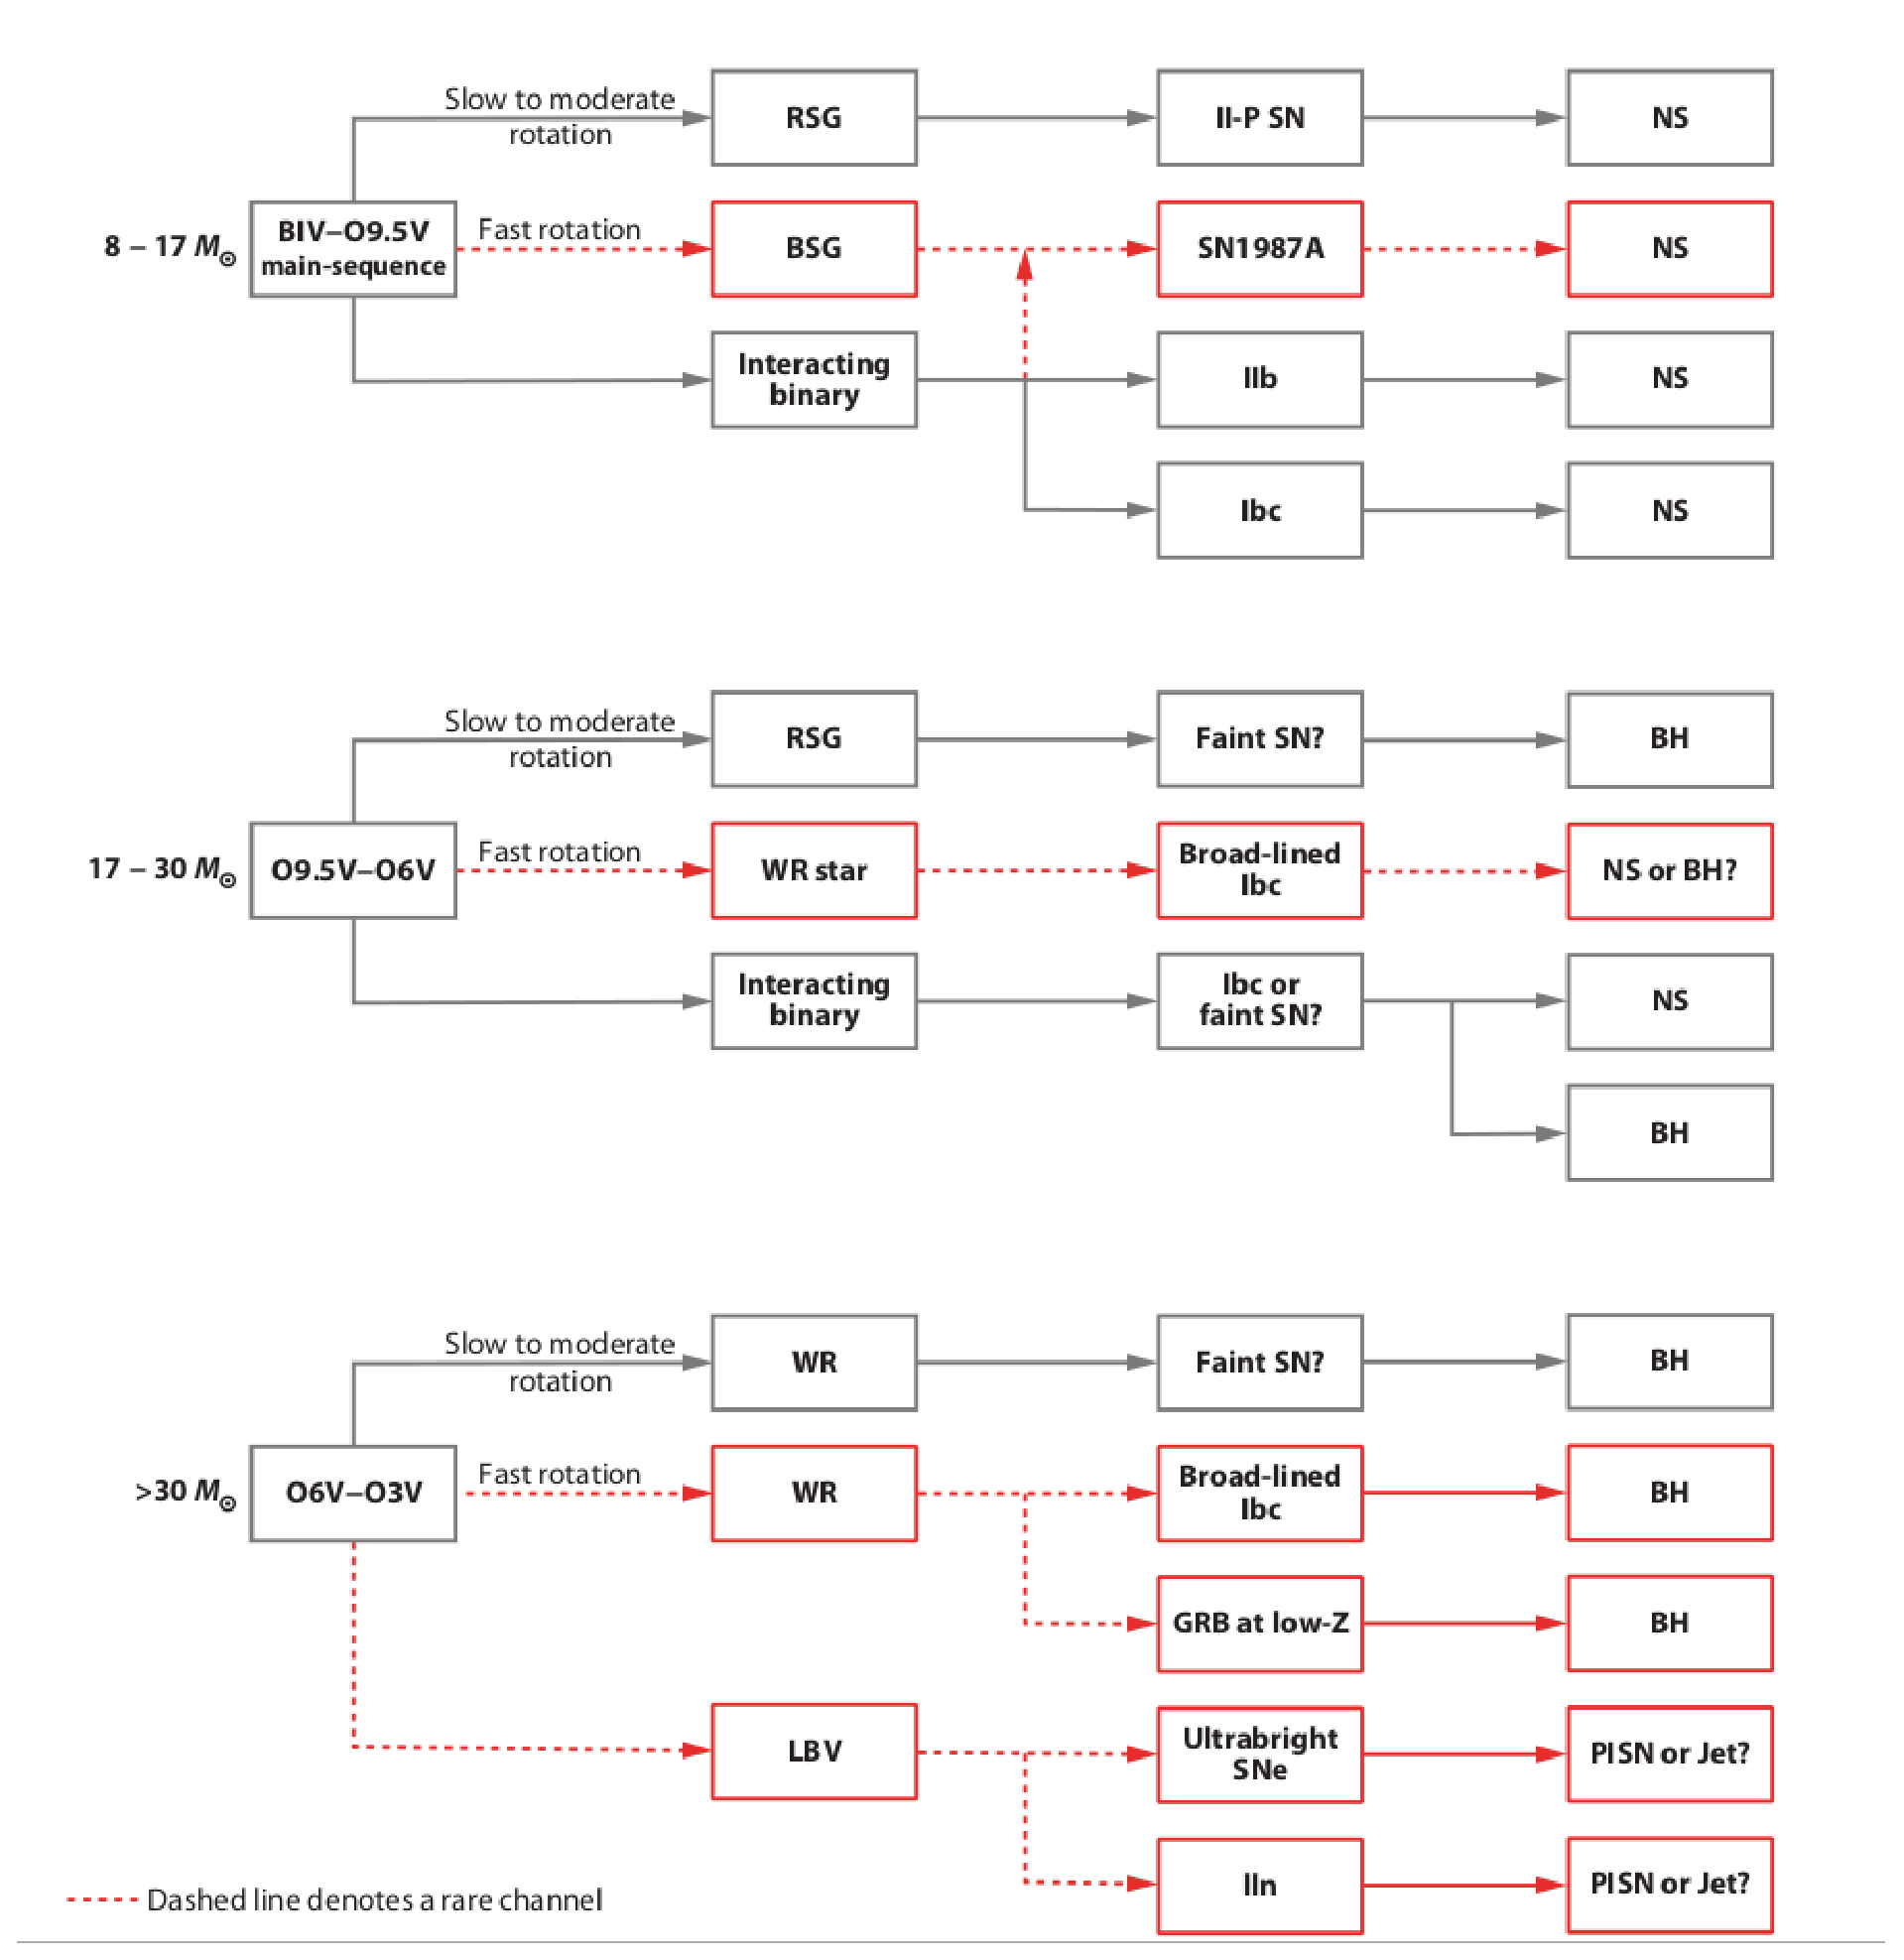
\includegraphics[width=0.65\textwidth]{intro/Smartt09fig12}
 \caption[HRD]{The evolutionary diversity of the end points of massive stars and their associated observed SN classification. Figure reproduced from~\cite{Smartt09}. Acronym definitions: RSG, red supergiant; BSG, blue supergiant; LBV, luminous blue variable; WR, Wolf$-$Rayet; NS, neutron star; BH, black hole; GRB, gamma-ray burst; PISN, pair-instability supernova.
 \label{fig:SNe-Smartt}}
\end{figure}

% subsection death (end)
% section the_life_of_a_red_supergiant (end)

\section{Chemical Properties of Red Supergiants} % (fold)
\label{sec:chemical_properties_of_red_supergiants}

\subsection{{\it J}-band Analysis Technique} % (fold)
\label{sub:subsection_name}

% subsection subsection_name (end)
\subsection{Galactic and Extragalactic RSGs} % (fold)
\label{sub:galactic_and_extragalactic_rsgs}

The intrinsic brightness of RSGs, particularly in the NIR, makes these stars popular candidates for observations within and beyond the Galaxy.
Studies of Galactic RSGs are used to derive fundamental stellar parameters such as radii, masses and distances.
Galactic RSGs are also a natural starting point for extragalactic studies of larger populations of RSGs.
Extragalactic observations have identified populations of RSG stars in a large range of galaxies within the Local Group and (in rarer cases) out to larger distances~\citep[e.g.][]{Elias85,Humphreys86, Massey06, 2007AJ....134.2474M, Groenewegen09,Massey13}. % how do I put "table 1 in massey"?
These studies provide important results on RSGs in different environments.
To illustrate this, this section first comments on some of the fundamental parameters derived using Galactic RSGs in Section~\ref{Galactic RSGs} and summarises some of the important observational results regarding extragalactic RSGs in Section~\ref{extragalactic RSGs}.
In Sections
\ref{selection} and
\ref{Galactic RSGs}, I focus on some of the aspects of extragalactic RSGs which will be applicable in later stages of this document.

\subsubsection{Fundamental Parameters in Galactic RSGs}\label{Galactic RSGs}

Research into Galactic RSGs is typically divided into two categories: studies of individual nearby stars such as Betelgeuse~\citep[$197\pm 45$pc;][]{Harper08} and VY CMa~\citep[$1420\pm$ 120pc;][]{Wittowski12} and studies of populations of RSGs within open clusters and associations~\citep[e.g.][]{Levesque05,Negueruela13}.
Studies of individual Galactic RSGs concentrate on the fundamental parameters of these stars such as their distances, mass-loss rates and circumstellar envelopes.
Additionally, nearby Galactic RSGs are tests for detailed stellar atmosphere and evolutionary models.

Observations of Galactic RSGs reveal that they have large mass-loss rates~\citep[10$^{-(6\pm 1)}$M$_{\odot}$yr$^{-1}$;][]{Danchi94, Richards13} and extended circumstellar environments~\citep{Smith01} which may containing masers~\citep{Schuster06}.
Mass loss during this phase of evolution is critical for the understanding of subsequent evolutionary stages as well as understanding SN progenitors.
%The remnant of SN 1987A displays loops which are thought to have origionated in mass loss events during the RSG phase of evolution of its progenitor star~\citep[][and references therein]{Humphreys13}.
Galactic RSGs act as an important sample to study and understand the mechanisms of mass loss, as extragalactic observations are unable to resolve the structure which can be seen in nearby Galactic stars.

One of the main uncertainties with studies of these nearby stars are the relatively poorly constrained distances (e.g., Betelgeuse with a distance uncertainty of nearly 25\%).
In order to (partially) remove the distance uncertainty problem, RSGs can be observed in Galactic clusters of known distances~\citep[e.g.][]{Humphreys78, Mel'Nik95}.
%% MS fitting, observe spectral type and fit cluster onto a HR diagram to estimate the absolute magnitude, distance modulus
This technique is useful to study large populations of RSGs which can be used to test theories of star formation and models of RSGs and their atmospheres.
Studies of RSGs in Galactic clusters are often used as a first test for studies which plan to include observations at larger distances~\citep[e.g.][]{Levesque05,Levesque06, 2010MNRAS.407.1203D,2013ApJ...767....3D}.

\subsubsection{Extragalactic Studies and Results}\label{extragalactic RSGs}

Extragalactic studies of RSGs are advantaged in that it is possible to accumulate large samples of RSGs with which to test stellar evolution theories and derive stellar parameters.
By using the different environments available in the Local Group, studies of extragalactic RSGs can probe a wide range of host galaxy parameter space.
For example, M31 (Z$>$1.0Z$_{\odot}$ in the central regions), a massive, metal-rich spiral galaxy and the Wolf$-$Lundmark$-$Melotte (WLM; Z=0.1Z$_{\odot}$), a dwarf irregular, metal-poor galaxy, both contain a significant population of RSGs.

Through an analysis of RSGs in different metallicity environments, various authors report that the average spectral type of a RSG population is dependent upon metallicity~\citep{Elias85, MasseyOlsen03, 2012AJ....144....2L}, where lower metal abundances give rise to earlier average spectral types.
%% Chris' comment:
%not necessarily - the way I always thought about this was that, e.g., in the SMC, the TiO bands are weaker, so for a given spectral type, the star needs to be cooler to reproduce the TiO strengths for, e.g. M3 or M4 types.  Thus, the coolest star could have the same Teff, but its spectral type will appear earlier.
In addition to this, RSGs can be used to measure abundances in Local Group galaxies, which yield important results by mapping metallicity gradients.
This work has typically been done using high-resolution spectra at NIR wavelengths~\citep{Cunha07, Davies09a,Davies09b}.
However, in order to optimise these studies,~\cite{2010MNRAS.407.1203D} adapted a method for determining the chemical properties of BSG stars in the optical~\citep{Kudritzki08,Kudritzki10}, to RSGs in the NIR.

Measurements of the temperatures of RSGs have also provided insight through using observations of extragalactic RSGs in the NIR.
The temperatures of RSG stars have been subject to debate for many years.
There are many methods by which to estimate the effective temperature of a RSG star.
The most popular of which is to fit the spectral energy distribution (SED) of the star with 1D model atmospheres~\citep{2008A&A...486..951G}.
However,~\cite{2013ApJ...767....3D} show that observations fitting models around the BVRI region, where molecular TiO lines dominate the absorption, result in a systematically lower temperature compared with fitting the line-free continuum regions of the SED.
This is due to the fact that the TiO molecular line forms higher in the atmosphere of the star than the continuum.
This means that fitting the TiO region and assuming that the best fitting effective temperature is representative of the entire SED is not a good assumption.
\cite{2013ApJ...767....3D} advocate using the entire SED \textit{except} those regions dominated by the TiO absorption features.
Deriving temperatures of extragalactic RSGs will be an important test for stellar evolution models and an excellent way in which to test models at different metallicities and in different environments.

In order to test models of stellar evolution against observations of extragalactic RSGs, a complete sample of RSG stars is clearly beneficial in order to draw conclusions on how the population behaves and evolves as a whole.
In order to do this, generally, stars must be selected for spectroscopic follow-up observations based on their photometric properties.
%Obviously, if an extensive stellar spectroscopic survey is available, this problem quickly disintegrates.
%However, in all other cases, photometric selection is an important factor in the study of extragalactic RSG stars.

%RSG have luminosities which can rival entire populations of stars ($> 10^{4.5-5.8}$L$_{\odot}$).
%But, unlike their hot progenitors, the peak wavelength of a RSG star is around 1$\mu$m, therefore, at NIR wavelengths, these stars dominate the light output from their host galaxies.

  % Radii, absolute magnitude ... useful?
  % Surface gravities?

  % Figure 8 from Massey 2003 and references therein
  % Figure 3 Levesque et al 2005
%% Levesque et al 2005 define a new temperature scale which brings the temperatues up
% Luminosities
% optical spectroscopy Massey, levesque, Drout etc
  % Winds/Mass loss rates
  %% Driven by radiation pressure~\citep{Langer12}
  % Rotation
%% Betelgeuse v=15kms^{-1} <-- is this a large rotation or not ... sun = 2kms^{-1}

  % Binary fraction
%% Sana et al 2012 \sim 70% of massive O stars are contained within binary systems Galactic
%% Sana et al 2013 \sim 50% of massive O stars are contained within binary systems 30 Dor (VFTS)

%% This is not true at all! circumstelalr material is very difficult to detect in RSGs (Harper et al. 2008; Smith et al.2009)
%Another property of the spectra of RSG stars which is useful in order to distinguish these objects from their lower mass counterparts is the presence of emission lines.
%These lines arise due to the circumstelar material surrounding all RSG stars.
%This circumstellar material arises from the strong winds which are characteristic of all RSGs and will be discussed further in Section~\ref{properties}.

\subsubsection{Photometric Selection of RSGs}\label{selection}

In the absence of spectroscopic observations, the selection of objects with respect to follow-up observations is often done using broad band photometry.
%Broad band observations typically use the standard Johnson-Cousins filters, UBVRIJHK(K$_{s}$).
This section will describe some of the various methods used to isolate a population of stars using magnitudes derived from broad band filters.
This is important as good photometric selection of targets can optimise observing strategies and should be able to provide a complete sample of the population of stars.

Colour$-$magnitude diagrams (CMDs) are often used to isolate a particular type of star.
A colour is defined as the difference between two magnitudes, derived from  two different filters, and colours trace the temperature of a star (and hence their spectral type), whereas magnitude can be used to approximate luminosity.
Therefore, using CMDs should allow the separation of a population of red, luminosity class I (supergiant), stars.
However, using this method assumes that the sample consists purely of one population of stars at a given distance; if this assumption is not true, apparent magnitude is no longer sensitive to luminosity.
For example, a nearby population of faint stars with similar spectral types (colours) could pose as a bright population of more distant objects.
This becomes important when viewing an extended extragalactic object, such as a stellar cluster or external galaxy, at low Galactic latitude where the Galactic stellar density is highest.
An example of a typical CMD is given in Figure~\ref{fig:CMD}.

 \begin{figure}
 \centering
 \includegraphics[width=0.65\textwidth]{intro/N6822_bvr}
 \caption[B$-$V, V]{Optical colour-magnitude diagram (CMD) of NGC 6822, in which the absolute V-band magnitude M$_{V}$, (corrected to the distance of NGC 6822) is plotted against B$-$V colour.
This figure illustrates how CMDs can be used to separate stars based on spectral type. Redder colours indicate later spectral types.
This figure also demonstrates that CMDs have inherent degeneracies  between different populations of stars: the central dense feature at B$-$V $\sim$ 1.0 is attributed to foreground contaminants
 \label{fig:CMD}}
\end{figure}

% \begin{figure}[t]
%   \begin{center}
%   \epsfxsize=150mm         % Horizontal size YOU want
%   \epsffile{bvcmd_all_example.eps}
%   \caption{Optical colour-magnitude diagram (CMD) of NGC 6822, in which the absolute V-band magnitude M$_{V}$, (corrected to the distance of NGC 6822) is plotted against B$-$V colour.
% This figure illustrates how CMDs can be used to separate stars based on spectral type. Redder colours indicate later spectral types.
% This figure also demonstrates that CMDs have inherent degeneracies  between different populations of stars: the central dense feature at B$-$V $\sim$ 1.0 is attributed to foreground contaminants.}
%     \label{CMD}
%     \end{center}
%  \end{figure}
 \begin{figure}
 \centering
 \includegraphics[width=0.65\textwidth]{intro/N6822_bvr}
 \caption[B$-$V, V$-$R]{Optical colour$-$colour diagram of NGC 6822. This figure illustrates the surface gravity dependence of the B$-$V colour at a given V$-$R colour. The population with the redder B$-$V colours contain the RSG objects.
 \label{fig:CCD}}
\end{figure}

% \begin{figure}[t]
%   \begin{center}
%   \epsfxsize=150mm         % Horizontal size YOU want
%   \epsffile{bvrccd_example.eps}
%   \caption{Optical colour$-$colour diagram of NGC 6822. This figure illustrates the surface gravity dependence of the B$-$V colour at a given V$-$R colour. The population with the redder B$-$V colours contain the RSG objects.}
%     \label{CCD}
%     \end{center}
%  \end{figure}

To break the degeneracy between luminosity and distance, one can use colour$-$colour diagrams.
Using multiple colour diagnostics can isolate stars based on more than just spectral type and absolute magnitude.
\cite{1998ApJ...501..153M} show that at a given V$-$R colour, the B$-$V colour is sensitive to the surface gravity of a star.
Therefore, given a V$-$R colour, RSGs can be isolated owing to their low surface gravity.
An example of such a colour$-$colour diagram is shown in Figure~\ref{fig:CCD} where one can clearly see the distinction between low surface gravity RSG stars (with slightly redder B$-$V colours) and the dwarf high surface gravity stars.

The selection of RSGs is typically done using a B$-$V, V$-$R colour$-$colour diagram as this diagram has had much success in selecting RSGs and is known to contain a small number of contaminants.
However, a potential issue with these diagrams as we move to extragalactic systems, which at the time of writing has not been quantified, is that RSGs are known to reside in dense regions and/or clusters with many bluer, younger stars.
When viewing these stars in the optical, the colours from RSGs could potentially be contaminated to bluer colours by the blue stars which also reside nearby.
In a B$-$V, V$-$R diagram, this contamination would affect the completeness of the population of RSGs selected.
As stated, this is not quantified and would require a comparison between the B$-$V, V$-$R selection method with another known selection method and an analysis of the locations of the potentially contaminated RSG stars.
A potential solution to this problem would be to select RSGs based on their NIR colours, which is where these stars are brightest and hence would be less subject to contamination to nearby blue objects.
% This argument could be reversed and in the NIR we could push blue stars towards our RSG targets. Would this be a problem?

Working in the NIR, authors have used the J, J$-$K CMD~\citep{2000ApJ...542..804N,2006A&A...452..195C,Neugent12} to select red stars (RSGs and asymptotic giant branch (AGB) stars) and much work has been done in identifying contaminants and the parameter space where individual populations reside in~\citep{2006A&A...452..195C}.
As mentioned above, the main contaminants with this selection method are foreground dwarfs.


% subsection galactic_and_extragalactic_rsgs (end)
% section chemical_properties_of_red_supergiants (end)

\section{Chemical Evolution of Galaxies} % (fold)
\label{sec:chemical_evolution_of_galaxies}

The evolution of galaxies is a vast field and can be broadly split up into three main fields: dynamical, thermal and chemical evolution.
%In reality these topics depend upon each other, but given certain crude approximation can to an extent be studied independently.
The chemical evolution of galaxies governs the origin and distribution of elements within the host galaxy.
This evolution principally depends upon galaxy and star formation.
The initial origin and distribution of the chemical elements depends upon the galaxy formation process.
Star formation acts to alter these quantities by creating, redistributing and removing chemical elements from the interstellar medium (ISM).

The lowest mass stars remove elements from the ISM by storing their gas and never evolving off the MS!
Stars massive enough to evolve off the MS eject some mass during an AGB phase, but subsequently end their lives by removing elements from the ISM as passively cooling white dwarf stars.
%These stars could also end up as Type Ia SNe
More massive stars undergo large amounts of mass loss during all phases of their evolution and end their lives by exploding as CCSNe, both of which act to alter the chemical composition of their surrounding gas clouds.

All three of these processes are important to take into account when studying how galaxies chemically evolve over time.
However, quantifying contributions from these quantities is an involved process, complicated by a minefield of caveats and uncertainties.

Extragalactic observations of fundamental properties of galaxies play important roles in refining theories of galaxy formation and evolution.
The mass$-$metallicity relationship~\citep[MZR;][]{Lequeux79} of galaxies combines two fundamental parameters of galaxies.
The stellar mass represents the amount of gas which star formation has removed from the ISM, whereas the present day galaxy metallicity represents how star formation has altered the initial ISM.
Various authors have shown that galaxy mass is proportional to metallicity~\citep{Tremonti04, Maiolino08,Kewley08}.
This relationship can be interpreted by considering multiple factors.
In low-mass galaxies, outflows and SNe have a greater affect on the amount of material ejected from the host galaxy into the intracluster medium, owing to their shallower potential wells~\citep[e.g.][]{Tremonti04}.
Additionally, low-mass galaxies represent an early stage in Galactic evolution and hence, these galaxies have not had time to process their gas into stars.
As the host galaxy evolves, subsequent episodes of star formation increase the metal content of the galaxy~\citep[e.g.][and references therein]{Maiolino08}.

MZR observations have typically relied upon ratios of strong oxygen emission lines (usually [OII], [OIII] relative to H$\beta$) from HII regions to derive metallicities of individual galaxies.
This technique is used due to its applicability over a large distance range:
\cite{2001MNRAS.323..887C} use this technique in nearby galaxies whereas \cite{Maiolino08} derive metallicity using this method in galaxies at z$>$3.
However, these measurements are known to be highly dependent upon the calibration method used~\citep{Kewley08, Kudritzki08,Bresolin09}.
In order to provide an independent calibration of this method, BSG stars have been used to determine metallicity and abundance gradients in external galaxies~\citep{Kudritzki12}.
In addition to this,~\cite{Davies13b} outline a method using RSGs as abundance probes with which to calibrate the MZR.
These authors show that using a NIR window around 1.2$\mu$m (J-band) the dominant spectral features are that of strong metallic lines of iron and alpha elements (Ti, Mg, Si).
These strong metallic lines allow abundance measurements from relatively low resolution spectra meaning that this technique can be used at distances of 3-4Mpc with an 8-10m class telescope (significantly, outside the Local Group).


Another advantage of using relatively low resolution spectra are that multi-object spectrographs can be used to observe extragalactic systems.
This provides not only reliable abundances in nearby galaxies but also spatial information about abundances in these galaxies which allows the determination of metallicity gradients.

Therefore, extragalactic observations of RSG stars are important in order to provide independent constraints on some of the fundamental properties of Galactic formation and evolution.
These studies have enormous potential in the era of extremely large telescope era which will be optimised for NIR observations.
% section chemical_evolution_of_galaxies (end)

% \chapter{Spectroscopy with the {\it K}-band Multi-Object Spectrograph}

\section{Introduction to Spectroscopic Techniques} % (fold)
\label{sec:introduction_to_spectroscopic_techniques}

Spectroscopy is the study of the dispersion of light into its constituents and has been at the forefront of astronomy for roughly the last 200 years.
Sir Isaac Newton demonstrated the principles of spectroscopy (and coined the term ``spectrum'') using light from The Sun in his seminal ``Opticks'' work~\citep{Newton16xx}.
By using the groove spacings on a diffraction grating, Thomas Young first quantified the wavelengths of different colours of light~\citep{Young1801}.
The simple set-up of a spectrograph, which has - more or less - been used since the early spectroscopic experiements, consists of five basic elements:

\begin{enumerate}
    \item Slit
    \item Collimator
    \item Dispersive element
    \item Camera
    \item Detector
\end{enumerate}

In Newton's demonstration he used a small hole in his window blinds as a slit and a screem as a detector.
The slit in modern spectroscopic observations can take various forms.
The most widely used type of slit, in modern observations, is long-slit spectroscopy.
Using a long slit, a spectrum is taken for each spatial pixel along the length of the slit.
This is demonstrated in Figure~\ref{fig:long-slit}, where the final panel shows that each pixel illuminated by the slit produces a spectrum.
This can be thought of a 2-dimensional spectroscopy, which is particualrly useful when attempting to take a spectrum of an extended object
(rather than a point source).

\begin{figure}
 \centering
 \includegraphics[width=0.65\textwidth]{kmos/xxx}
 \caption[Long-slit Spectrscopy]{Three panels demonstrating long-slit spectrscopy
 \label{fig:long-slit}}
\end{figure}

As an alternative to using a long-slit to remove contamination from other sources, is to use a small hole or fibre to select the target flux.
By precisely drilling a hole in a metal plate, a slit is created which can be used to select the target flux.
One of the advantages of using this method is that more than one object can be selected for a single exposure.
By creating multiple slits within a single plate, spectroscopy from multiple objects can be obtained where contamination from other sources is minimised.
An improvement to this method was to use optical-fibres positioned within the holes.
The fibres could then be led to an instrument which was not directly attached to the telescope, which has the advantage that the instrument will not suffer from the changing gravitational force as the telescope moves.
In addition, the conditions within the instrument room can be controled.
This is particularly important for near-IR spectrographs and detectors.

However, using a plate with several holes drilled into it has some drawbacks.
These include the time in which it takes to create the slit mask, the lack of flexibility while observing and the operational costs of creating a new mask each time a different field is to be observed~\citep{1986SPIE..627..118P}.
These reasons, in addition to improved computing power, led to the development of instruments which were able to automatically position fibres~\citep{1982SPIE..331..289T}.
Most modern fibre-fed spectrographs have automatic fibre positioning technology which is broadly split up into two approaches.

\begin{enumerate}
    \item Each fibre has a magnetic button attached and a single robot is charged with moving each fibre sequentially.
    This is an effective method to place large numbers of fibres, but does however, take a significant length of time for each configuration.
    \item Each fibre is mounted upon a computer controlled arm.
    This method is generally less time consuming.
\end{enumerate}

As a variant on the five basic elements of a spectrograph, slitless spectroscopy is also a feasible option which is not discussed in detail here.
For more information on slitless spectroscopy see Fergus' thesis!

\begin{figure}
 \centering
 \includegraphics[width=0.65\textwidth]{kmos/xxx}
 \caption[Long-slit Spectrscopy]{Three panels demonstrating long-slit spectrscopy
 \label{fig:long-slit}}
\end{figure}


Dispersive elements ...
\begin{itemize}
    \item Compare prims and diffraction gratings ()
    \item Describe diffraction gratings in detail and how they are made
    \item Why do different gratings select different wavelengths?
\end{itemize}

Camera ...
\begin{itemize}
     \item Brief mention, if at all.
     \item Focuses the light again
 \end{itemize}

Detector ...
\begin{itemize}
    \item Brief comments on specialisations for near-IR
    \item i.e. Cooled etc.
\end{itemize}


Young, T., Phil. Trans. R. Soc. 92, 12 (1802)

% The resulting spectrum, which the detector records, is typically of the form of an intensity Vs. wavelength diagram for the target source.
% The features which are recorded are referred to as absorption or emission features.
% Fundamentally, these features are so useful for astronomical observations as they arise owing to the properties of the chemical elements.
% Each atom, and in turn molecule, has a unique spectrum which allows astronomers to identify atmos and molecules present in the observed target.
% By comparing the shape and strength of different spectral features (against laboratory measurements) one can estimate the physical parameters of the target (see Chapter~\ref).




% A spectrum of a star can be obtained by passing the light the telescope collects from the star through a prism or, more commonly used at modern observatories, a grism.
% These instruments disperse light by exploting the properties of light as a wave.
% A prism disperses light using the refractive properties of light as a wave through a triangular shaped chunk of glass (i.e. prism shaped).
% JWST NIRSpec will have a prism

% A diffraction grating was used to disperse light by Thomas Young
% A diffraction grating improves spectral resolution and allows wavelength to be quantified
% A grism disperses light using a highly posished reflective surface with ridges at defined intervals.
% Stuff on prisms and grisms (figures showing two examples -- do I have any photos of grisms from la Palma?)
% \begin{itemize}
%     \item Why do we use grisms rather than prisms?
%     \item Did astronomers ever use prisms?
% \end{itemize}


% The idea that one exposure from a telescope can lead to multiple spectra, so called multi-object spectroscopy, is a more recent addition to the arsenal of the astronomer.
% Talk about some previous multi-object spectrographs. AAOmega? AF2? FORS2? etc.


\section{Integral field spectroscopy} % (fold)
\label{sec:integral_field_spectroscopy}

% section integral_field_spectroscopy (end)
How exactly does IFU spectrosocpy work again \ldots?

\begin{itemize}
    \item Image slicer!
\end{itemize}

% section introduction_to_spectroscopic_techniques (end)

\section{Instrument} % (fold)
\label{instrument}

% section the_instrument (end)

\section{Data} % (fold)
\label{data}

% section data (end)
\section{Data Reduction} % (fold)
\label{data_reduction}

% section data_reduction (end)

\section{Conclusions} % (fold)
\label{sec:conclusions}

% section conclusions (end)
% %%%%%%%%%%%%%%%%%%%%%%%%%
% Set up to be stand alone document
% All declerations in the header to be removed when added into thesis
%%%%%%%%%%%%%%%%%%%%%%%%%
% \documentclass[12pt]{article}

% \usepackage{booktabs} % booktabs provides professional formatting commands for tables
% \usepackage{amsmath} % amsmath provides extra maths symbols
% \usepackage{textcomp} % textcomp provides extra text symbols (like a degrees celsius symbol)
% \usepackage{../customisations}
% \usepackage{natbib}

% \title{$J$-band Sythentic Spectral Fitting}
% \date{\today}

% \begin{document}
% \maketitle
%%%%%%%%%%%%%%%%%%%%%%%%%
% To be included when added into thesis
\chapter{J-band Spectral Analysis}\label{ch:janal}

\section{Opening Remarks} % (fold)
\label{sec:opening}

In this chapter I describe in detail the process by which I implement an analysis
routine to fit synthetic spectra to observed data with the aim of estimating stellar parameters.
This analysis builds on existing methods while providing a fresh approach to various aspects of the routine.
I have developed this implementation in the public domain and the source code for this project is made publicly available
via an online repository.\footnotemark

\footnotetext{Source code available from: https://github.com/lrpatrick/rsg-janal
although the interested reader should be aware that these routines are, at the time of writing, in development mode
in the sense that they are highly specialised to one machine and (particularly) one set of model grids}

In this chapter I first outline the principles of model atmospheres in Section~\ref{sec:model_atmospheres}, where I discuss the physics which is included in these models as well as some of their strengths and limitations.
I then focus the discussion on the grid of synthetic stellar spectra which forms the base of this analysis routine in Section~\ref{sec:model_grid}.
In Section~\ref{sec:continuum_fitting} I detail the procedure of matching the continuum level of the observations with that of the models,
which leads on to Section~\ref{sec:best_fit_parameters}, where the method by which the best fit parameters are selected is described.

Having described the analysis routine thoroughly I then test this routine and compare the results of this method to different implementations in the literature in Section~\ref{sec:calibration}.
Finally, I conclude the chapter in Section~\ref{sec:conclusions}.

% section opening (end)
\section{Introduction to Stellar Model Atmospheres} % (fold)
\label{sec:model_atmospheres}

A stellar atmosphere is defined as the outer layers within a star which emit radiation.
Therefore, by definition, the photons which we observe from a star have originated in the atmosphere.
Photons which have originated from deeper layers within the star have been absorbed and re-emitted by particles within the stellar atmosphere.
Stellar atmospheres are therefore vitally important in observational studies of stars, even though the fraction of the total mass of the star contained within the atmosphere is tiny ($\sim$~10$^{-10}$).
A nice analogy for visualising this layer and its thickness comes from the preface of~\cite{1989isa2.book.....B}, where these authors compared the skin of an apple to a hypothetical star which has been shrunk to the same scale and note that the skin of the apple is far thicker than the stellar atmosphere.


Even though stellar atmospheres contain a tiny fraction of the total stellar mass, these layers can have an enormous impact on the evolution of a star via stellar winds.
For example, in evolved massive stars, winds arising from the atmosphere can strip off the outer layers of the star to leave an exposed hydrogen and helium dominated core or push the star in a completed different evolutionary direction to become a RSG (see Chapter~\ref{ch:intro}).
In addition to having an impact on the evolution of the star, winds also help distribute material throughout their host galaxy and feed subsequent generations of star formation~\citep[e.g.][]{2011MNRAS.417..950H,2012MNRAS.421.3522H} thereby not only affecting the evolution of the star in which the wind is produced, but by acting as part of a larger stellar population, affect the evolution of their host galaxy.

By modelling stellar atmospheres, one can estimate fundamental stellar parameters by a comparison with observations.
The background theory and underlying physical assumptions of these models is the subject of the current section.
This is important to detail as without this background it is impossible to assess the effectiveness of the models and their limitations.

Two of the most fundamental equations which govern the properties of stellar atmospheres are,

\begin{equation}
    g = \frac{GM}{R^2},\label{eq:grav}
\end{equation}

\noindent and,

\begin{equation}
    \Teff = \frac{F}{\sigma_{SB}} = \left(\frac{L}{4\pi \sigma_{SB}R^2}\right)^\frac{1}{4},\label{eq:Teff}
\end{equation}

\noindent where $g$ is the acceleration due to gravity, $M$ is the total mass of the star of radius $R$, \Teff is the effective temperature of the star, $F$ is the total flux per unit area, $L$ is the total luminosity of the star, $\sigma_{SB}$ is the Stefan-Boltzmann constant and $G$ is Newton's gravitational constant.

These equations define some fundamental observational properties of the model stellar atmospheres.
Equation~\ref{eq:grav} is defined by the density stratification of the model and equation~\ref{eq:Teff} is defined through the total flux emitted from the model.

In the following sections I detail three of the principle assumptions which are used to create a ``classical'' one dimensional stellar model atmosphere.
These assumptions underpin some of the most widely used model atmospheres.


\subsection{Hydrostatic Equilibrium} % (fold)
\label{sub:hydrostatic_equilibrium}

Any model of a star consists of a balance between gravity and pressure in a gaseous material (or plasma considering the typical temperatures and densities within a star).
If a model is assumed to be static (i.e. not varying with time) the equation of hydrostatic equilibrium can be derived by considering the balance between forces acting upon a small element of stellar material,

\begin{equation}
    \frac{dP(r)}{dr} = -\frac{\rho GM(r)}{r^2},\label{eq:hydro}
\end{equation}

\noindent where $P$ is the total pressure exerted within a radius $r$, $M$ is the total mass within a radius $r$, $\rho$ is the matter density~\citep[see Chapter 9 of ][for a simple derivation of this equation]{1989isa2.book.....B}.
As stated above, the mass contained within the atmosphere of a star is a negligible fraction of the total mass, therefore $M(r) = M_{tot}$ when considering this equation in the outer layers of the star.

The force exerted by pressure acting on an element of stellar material ($dP/dr$) can be considered as the sum of the forces acting upon it from gas pressure ($P_{g}$), radiation pressure ($P_{rad}$) and turbulent pressure ($P_{turb}$),

\begin{equation}
    \frac{dP_{tot}}{dr} = \frac{dP_{g}}{dr} + \frac{dP_{rad}}{dr} + \frac{dP_{turb}}{dr}.\label{eq:pressure}
\end{equation}

Equation~\ref{eq:pressure} illustrates that even though we have assumed the model is static, small scale turbulent motions must still be taken into account to accurately model stellar atmospheres.


% subsection hydrostatic_equilibrium (end)

\subsection{Mixing Length Convection} % (fold)
\label{sub:mlt}

Mixing length theory describes how convection is treated within the stellar atmosphere.
Typically, within a star, radiation is the main source of energy transport as the coefficient of diffusion is far smaller for particles (conduction) than for photons (radiation).
Only in degenerate cores does energy transport via conduction become important.

Convection is a very efficient form of energy transport where a macroscopic element of higher temperature rises an average distance into a region of lower temperature where it dissipates the excess energy being carried and mixes.
However, in order for convection to be effective, a driving mechanism must be established.
The atmosphere is unstable to convection if the Schwarzschild criterion is met,

\begin{equation}
    \nabla_{rad} > \nabla_{ad}
\end{equation}

\noindent where $\nabla_{rad} = (d~{\rm ln}\,T/d~{\rm ln}\,P)_{rad}$ is the radiative temperature gradient and $\nabla_{ad}$ is the adiabatic temperature gradient.
The driving mechanism for convection is usually a large temperature gradient within a particularly part of the star.
This can occur at various stages within the lifetime of a star, for example, most main sequence stars have a convective core which is a result of the temperature sensitivity of the CNO cycle which establishes a steep temperature profile.

The theory of convection is very difficult to to treat thoroughly.
The ``simple'' theory of mixing length convection~\cite{1958ZA.....46..108B,1965ApJ...142..841H} is widely used to implement convection within stellar atmospheres which assumes that the shapes and sizes of the elements which transport energy is fixed and that, on average, an element rises a characteristic length ($l_m$) before it dissipates energy.

If the Schwarzschild criterion is satisfied, the total flux ($F$) for a star is given by,

\begin{equation}
    F(r) = F_{conv} + F_{rad} = \sigma T_{eff}^4,\label{eq:flux}
\end{equation}

\noindent where $F_{conv}$ and $F_{rad}$ are the convective and radiative flux respectively.
An expression for the convective flux can be obtained by considering the excess energy dissipated by a rising element moving a distance
($\Delta r = l_m/2$) with an average velocity ($v_{conv}$).
The convective flux can therefore be expressed as,

\begin{equation}
    F_{conv} = \rho C_pv_{conv}\Delta T,
\end{equation}

\noindent where $C_p$ is the specific heat at constant pressure and $\Delta T$ is the temperature difference between the element and surroundings, which can be expressed in terms of the different in temperature gradients.
Here the pressure scale height can be introduced using the assumption of hydrostatic equilibrium $H_p = dr / d{\rm ln} P = p/\rho g$ and an expression for the convective velocity can be estimated by assuming that half the work done by buoyancy is converted into kinetic energy,

\begin{equation}
    \frac{1}{2}\langle w\rangle \approx \frac{1}{2}\rho v_{conv}^2.
\end{equation}

The parameter $\alpha = l_m/H_p$ is introduced which typically takes the value $\alpha$ = 1.5--2.0.
As a side note, in stellar evolutionary models, the value of $\alpha$ used can have a significant effect on the temperature of the models at the end of the RSG phase of evolution.


% subsection mlt (end)

\subsection{Local Thermodynamic Equilibrium} % (fold)
\label{sub:local_thermodynamic_equilibrium}

The assumption of thermodynamic equilibrium is where the temperature and density of a material can be considered constant (i.e. there are no net flows of energy).
Which is equivalent to assuming that the emitting source is a perfect black body.
Local thermodynamic equilibrium (LTE) is an approximation whereby the {\it local} properties of material can be assumed to be in thermodynamic equilibrium.
Stellar atmospheres can be approximated to be in LTE as their densities are sufficiently high and density gradients are sufficiently low that their local properties are closely related to thermal equilibrium.

The three fundamental equations which can be defined assuming LTE are:

\begin{enumerate}
    \item The Boltzmann equation,
    \begin{equation}
        \frac{n_i}{N_I} = \frac{g_i}{U_I}e^{-E_i/kT},\label{eq:boltz}
    \end{equation}
    \item The Saha equation,
    \begin{equation}
        \frac{N_I}{N_{I+1}} = n_e\frac{U_I}{U_{I+1}}\left(\frac{h^2}{2\pi m_ekT}\right)^\frac{3}{2} e^{\chi/kT},
        \label{eq:saha}
    \end{equation}
    \item The Maxwellian distribution of particles,
    \begin{equation}
        f(v)dv = \left(\frac{m}{2\pi kT}\right)^\frac{3}{2} \exp\left(\frac{-mv^2}{2kT}\right)4\pi v^2dv,
        \label{eq:max}
    \end{equation}
\end{enumerate}

\noindent where $n_i$, $g_i$ and $E_i$ are the population, statistical weight and energy of level $i$ respectively,
$N_I$, $U_I$ and $\chi_I$ are the total number density, partition function and ionisation potential of ionisation state $I$ (to which $i$ belongs),
$m$ is the mass of the particle, $v$ is the velocity of the particle, $T$ is the temperature of the particle and $k$ is the Boltzmann constant.
Equation~\ref{eq:boltz} determines the level population of a particular ionisation state for a given atom and in combination with the Saha ionisation equation (equation~\ref{eq:saha}) is used to determine the total level population for a given atom.

% These three equations describe the


% In addition the radiation source function (in the MARCS models -- not always the case) is assumed be be

% \begin{equation}
%     S_\lambda = \frac{\kappa_\lambda}{\kappa_\lambda + \sigma\lambda}B_\lambda(T) + \frac{\sigma_\lambda}{\kappa_\lambda + \sigma\lambda}J_\lambda
% \end{equation}

% More generally, in thermodynamic equilibrium $S_\lambda = B_\lambda$.
% In LTE

% subsection local_thermodynamic_equilibrium (end)

\subsection{Analysis of Assumptions and Summary} % (fold)
\label{sub:assumptions_summary}

The assumptions listed above allow one to obtain to create a ``standard'' stellar model atmosphere.
The assumptions listed above are known to be simplifications of the true picture with a stellar atmosphere.
For example, the assumption of LTE definitely breaks down in the atmospheres of stars as they are observed and, by definition, emit radiation.
However, using the above assumptions one can build a consistent model that, in general, agrees reasonably well with observations.

The treatment of convection is knowingly a large simplification as the shape and size assumed for the convective elements is constant whereas in reality the shapes of these elements could be described as funnel-like.
Full two- and three-dimensional hydrodynamical simulations are required to assess the assumption of mixing length convection which generally show that convective fluxes are smaller than those in more sophisticated prescriptions
\citep{2012sse..book.....K}.

The assumption of LTE typically holds in dense low levels of a star, however, in the atmosphere, where radiation is emitted, this is known to be a poor approximation.
This is particularly true in evolved stars where departures from LTE are expected owing to the low densities and surface gravities of their atmospheres.

Full non-LTE stellar model atmospheres are expensive to produce and are only available for particular sets of stellar parameters~\citep[e.g. {\sc tlusty} for stars with \Teff~$<$~27\,500;][]{2003ApJS..146..417L}
as of yet, there exists no homogeneous grid of model atmospheres which include these effects for cool stars.
As a first step, one can use a homogeneous set of model grids computed in LTE and select particular elements with which to compute non-LTE deviations in a particular wavelength regime.
This is far less time expensive and produces reliable results over a large range of stellar parameters.


% subsection analysis_of_assumptions_and_summary (end)

% section model_atmospheres (end)

\section{Quantitative Analysis of near-IR Spectroscopic Observations} % (fold)
\label{sec:model_grid}

To compare stellar model atmospheres to near-IR spectroscopic observations, synthetic spectra are calculated.
By calculating synthetic spectra from a grid of model atmospheres with a range of physical parameters, one can then compare the models to observations and determine the model, and hence stellar parameters, which best reproduces the data.
There are four model parameters which are considered to affect the appearance of the spectra:
global metallicity ($\log (Z/Z_{\odot})$~=~[Z]), effective temperature (\Teff), surface gravity ($\log\,g$) and microturbulence ($\xi$).
Microturbulence is a non-thermal velocity which is included in quantitative analyses of stellar spectroscopic observations in order to fit the observed line profiles.
For MS stars, empirical microturbulence velocities are thought to be connected with convective overshoot motions in stellar atmospheres~\citep{2009A&A...499..279C} and/or the result of high-order non-radial pulsations~\cite[e.g.][]{2015ApJ...806L..33A}.


The synthetic spectra used in this analysis cover the $J$-band, specifically the $1.16-1.22\mu$m region.
The wavelength range is chosen based on the spectral appearance of the region.
Typically, in the spectra of cool stars, dense molecular absorption features dominate the spectrum which require high-resolution spectroscopy to distinguish individual features and estimate stellar parameters~\citep{Cunha07, Davies09a, Davies09b}.
However, in this small wavelength range the absorption is dominated by well separated elemental absorption features from iron, magnesium, silicon and titanium.
Therefore, the spectral resolution required in order to derive stellar parameters is significantly reduced.
This means that this analysis, unlike others at higher resolution, can be performed with a relatively small amount of telescope time using near-IR multi-object spectrographs like KMOS on the VLT
or the multi-object spectrometer for infra-red exploration (MOSFIRE) on Keck and is therefore feasible for studies of large populations of RSGs in external galaxies.

In addition to this, given the cool temperature of the outer layers of RSGs,
the peak brightness of a typical RSG is $\sim\,1.1\mu$m.
Combining this with the fact that dust attenuation is significantly lower in the near-IR, compared to the optical regime, RSGs are ideal candidates to be studied at large distances.

At near-IR wavelengths, the effects of absorption and emission from the Earth's atmosphere is a considerable complication.
Although an absorption line may be strong and well separated from other stellar features, it may be contaminated by features arising from the Earth's atmosphere.
If a stellar feature is contaminated with strong absorption or emission arising from the Earth's atmosphere (telluric or sky line respectively), the correction required to divide or subtract the non-stellar feature may well leave behind residuals which perturb the line strength or shape.
For example, in Figure~\ref{fig:tell3pan} there are two strong iron lines around 1.16\,$\mu$m in the synthetic spectrum (top panel) which are well separated and would be suitable for the estimation of stellar parameters.
However, when telluric contamination is taken into account, we can see that the size of the telluric absorption around these lines is comparable to the strength of the lines (middle panel).
By correcting for the effects of the Earth's atmosphere we introduce a significant uncertainty in the strength and shape of these lines.
Therefore, these lines are unsuitable to be used to measure stellar parameters.
Equally, Figure~\ref{fig:skysub} in Chapter~\ref{ch:kmos} demonstrates the sky emission lines can also leave behind significant residuals that can perturb stellar features.
The diagnostic features therefore must be chosen carefully by examining not only the model RSG spectra, but by also taking into account potential reduction residuals arising from the Earth's atmosphere.
However, if one observes above the Earth's atmosphere, these lines - and many others - could be used to estimate stellar parameters.

\begin{figure}
 \centering
\includegraphics[width=\textwidth]{JAnal/tell-correction}
\caption[Three panels showing the effect of telluric absorption on spectral lines]{
Three panels showing the effect of telluric absorption on spectral lines.
The top panel shows a synthetic RSG spectrum within the wavelength of interest.
The middle panel shows a spectrum of the Earth's atmosphere and
the bottom panel shows an observed KMOS spectrum without telluric correction which is a combination of the top two panels and a noise spectrum.
To illustrate that the lines used in the analysis must come from regions where there is little telluric contamination, I draw the readers attention to the two iron lines at 1.16\,$\mu$m.
Even though these lines are well separated in the model spectra, telluric contamination renders these lines unsuitable for the estimation of  stellar parameters and one can see that the shape of these lines is altered by strong telluric contamination.
\label{fig:tell3pan}
         }
\end{figure}

% Previous studies which have used this wavelength regime to estimate stellar parameters for RSGs consist of that of
% \cite{2010MNRAS.407.1203D} and~\cite{2014PhDT.........G}.
% This implemenation includes aspects of both of these previous implementations and could be described as a hybrid of the two.
% Eventually this analysis routine will be made publicly available will should encourage the community to engage with these routines.

The synthetic spectra used in this analysis are calculated from model atmospheres computed from the MARCS model atmospheres project
\citep{1975A&A....42..407G,2008A&A...486..951G}.
These model atmospheres are ``standard'' type models computed in one-dimension (i.e. spherically symmetric)
where hydrostatic equilibrium, mixing-length theory of convection and LTE are assumed.
The MARCS models are particularly general and widely applicable to many different types of stars and as such are well used and tested.
However, for the atmospheres of RSGs the assumptions which go into these models (LTE in particular) are known to break down
\citep{2002AN....323..213F,2010ASPC..425..124P}.
Therefore, in order to accurately analyse the spectra of RSGs additional corrections must be applied~\citep{2012ApJ...751..156B}.

The MARCS model atmospheres used for this analysis are computed with a mass of 15\,M$_{\odot}$.
The typical mass range of a RSG is 8~$\leq$~M/M$_{\odot}$~$\leq$~40, however,
using this mass is applicable owing to the fact that altering the mass of these models affects only the extension
(or geometrical thickness) of the atmosphere which does not change substantially for red giants or supergiants
\citep[see][]{2010MNRAS.407.1203D}.

To improve the accuracy of the model atmospheres,
non-LTE calculations have been performed for all elements which give rise to the diagnostic features within the wavelength range studied
\citep{2012ApJ...751..156B,2013ApJ...764..115B,2015ApJ...804..113B}.
The line formation calculations of all known transitions of important atoms and molecules are computed in non-LTE using the {\sc detail} code~\citep{1981PhDT.......113G}.
{\sc detail} is a well tested and widely used code which is used to solve statistical equilibrium equations to obtain non-LTE level populations.
Using these level populations, line profiles and synthetic spectra -- with non-LTE corrections for the key diagnostic lines -- are calculated using an updated version of the {\sc SIU} code~\citep{1999PhDT.........3R,2012ApJ...751..156B} which employs the same input physics as {\sc detail}.
By calculating synthetic spectra from a grid of stellar models one can then evaluate which combination of model stellar parameters best represents the observed dataset.

The parameters of the resulting grid of synthetic spectra are detailed in
Table~\ref{tb:grid} where the spectral resolving power is $R$~=~10\,000,
which is significantly higher than the typical resolving power of the observed spectra
(i.e. $R \sim 3000$).
The sensitivity of each diagnostic line for a given free parameter is illustrated in Figures~\ref{fig:mod-z} through~\ref{fig:mod-micro} where one parameter is varied and the remaining are fixed.

\begin{table}
\caption{Model grid parameter space\label{tb:grid}}
\scriptsize
\begin{center}
\begin{tabular}{lccc}
 \hline
 \hline
Parameter & Abbreviation & Range & Increment \\
 \hline
Global metallicity & $[Z]$ & +1.0~--~$-$1.0 & 0.1\,dex \\
Effective Temperature & \Teff & 3400~--~4400 & 100\,$K$ \\
Surface gravity & $\log g$ & +1.0~--~$-$1.0 & 0.25\,dex \\
Microturbulence & $\xi$ & 1.0~--~5.0 & 0.2\,$km\,s^{-1}$ \\
 \hline
\end{tabular}
\end{center}
\end{table}




\begin{figure}
 \centering
\includegraphics[width=\textwidth]{JAnal/varyZv2}
\caption[An example of the effect of metallicity on the appearance of the model gird spectra]{
Three example models where only the metallicity is varied, the remaining stellar parameters are fixed at \Teff = 3900\,K, $\log g$ = 0.0 and $\xi$~=~3.0\kms.
Five diagnostic lines are shown in the two panels.
Left: Fe\,I $\lambda$1.188285 and Ti\,I $\lambda$ 1.189289.
Right: Fe\,I $\lambda$1.197305 and Si\,I $\lambda\lambda$ 1.198419, 1.199157.\label{fig:mod-z}
         }
\end{figure}
\begin{figure}
 \centering
\includegraphics[width=\textwidth]{JAnal/varygv2}
\caption[An example of the effect of surface gravity on the appearance of the model gird spectra]{
As in Figure~\ref{fig:mod-z} where surface gravity is varied and the remaining parameters are fixed at [Z] = $-$0.5, \Teff = 3900\,K and $\xi$~=~3.0\kms.\label{fig:mod-g}
         }
\end{figure}


From an analysis of Figures~\ref{fig:mod-z} and~\ref{fig:mod-g} it can be seen that the effect of increasing the metallicity of the models is similar to that of decreasing the surface gravity.
It is therefore expected that a degeneracy exists between metallicity and surface gravity.
This degeneracy is explored further in Section~\ref{sec:best_fit_parameters}.

The effect of varying the temperature of the models changes the relative strengths of the lines of different spectral species.
For example, see the left panel in Figure~\ref{fig:mod-t} where the ratio of the iron
($\lambda\,1.188285$) to titanium ($\lambda\,1.189289$) lines is strongly affected by varying the temperature of the models.
Also note that each species does not respond linearly to temperature.
This can be seen by a comparison between the strength of the iron line
($\lambda\,1.197305$) in the right hand panel of figure~\ref{fig:mod-t} to that of the silicon lines
($\lambda\lambda\,1.198419, 1.199157$) in the same panel.
This is clearly distinguishable from all the effects of all other parameters.


Increasing the microturbulence has the effect of increasing the equivalent widths
of the strongest lines preferentially as well as affecting the relative strengths of the lines arising from the same spectral species.
Therefore, strong features arising from the same element will be most sensitive to this
parameter.
This is illustrated by a comparison between the two strong iron lines
($\lambda\lambda\,1.188285, 1.197305$) in the left and
right panel of Figure~\ref{fig:mod-micro}.
Where the iron line in the left panel is strongest at $\xi~=~1.0$,
whereas at $\xi~=~5.0$, the iron line in the right panel is the stronger of the two.
In addition, the relative strengths of the two silicon lines
($\lambda\lambda\,1.198419, 1.199157$) in the right hand panel are not strongly affected, which illustrates that microturbulence preferentially affects the strongest spectral features.

\begin{figure}
 \centering
\includegraphics[width=\textwidth]{JAnal/varyTv2}
\caption[An example of the effect of effective temperature on the appearance of the model gird spectra]{
As in Figure~\ref{fig:mod-z} where effective temperature is varied and the remaining parameters are fixed at [Z] = $-$0.5, $\log g$ = 0.0 and $\xi$~=~3.0\kms.\label{fig:mod-t}
         }
\end{figure}
\begin{figure}
 \centering
\includegraphics[width=\textwidth]{JAnal/varymicrov2}
\caption[An example of the effect of microturbulence on the appearance of the model gird spectra]{
As in Figure~\ref{fig:mod-z} where microturbulence is varied and the remaining parameters are fixed at [Z] = $-$0.5, \Teff = 3900\,K and $\log g$ = 0.0.\label{fig:mod-micro}
         }
\end{figure}

The current model grid is sufficient to explore the parameters for a typical RSG in the Local Universe.
However, when using this technique at larger distances,
many different metallicity environments are encountered e.g. the low metallicity environment of I\,Zw\,18 with $Z=(1/32)Z_{\odot}$~\citep{1998ApJ...508..248V}.
In order to study these extremely low-metallicity systems,
the metallicity parameter space would need to be extended.
The $\alpha$-to-iron ratio of these stars is taken to be that of the solar value and is not yet left as a free parameter in the models.
This is applicable as young stars are known to have solar-like $\alpha$-to-iron ratios in different metallicity galaxies
~\citep[see tables 3 and 4 in][and references therein]{2015ApJ...806...21D}.

% section model_grid (end)
\section{Continuum Fitting} % (fold)
\label{sec:continuum_fitting}

Accurately matching the continuum levels in the observed
spectrum provides a base with which to anchor the comparison of the diagnostic lines of the models.
An incorrectly placed continuum level would bias the analysis and result in the
strength of the diagnostic lines being over- or under-estimated producing inaccurate stellar parameters.

% The continuum fitting procedure is important because determining the base of the
% diagnostic lines defines their overall strength which is used to distinguish
% between models.
There are many factors that affect the level of the continuum and continuum placement,
including the resolution of the observations as well as the stellar parameters themselves.
Therefore it is vital that when attempting to derive stellar parameters,
in crowded spectral regions such as this, the continuum placement is performed
consistently and accurately.
Intrinsically, when studying RSGs at medium resolution --- owing  to their cool atmospheres ---
there are many instances of blended spectral features.
At this resolution the density of blended spectral features creates a pseudo-continuum which, in practice,
is never at the true continuum level.
Figure~\ref{fig:mod-res} illustrates the varying continuum levels for models where the resolution is varied and
Figures~\ref{fig:mod-z}--\ref{fig:mod-micro} show that varying each of the stellar parameters affect the continuum in a subtly different manner.

\begin{figure}
 \centering
\includegraphics[width=0.65\textwidth]{JAnal/Resolution}
\caption[An example of the effect of the spectral resoltuion on the appearance of the model gird spectra]{
One model degraded to four different resolution values.
This figure demonstrates the how the continuum level changes depending upon
the resolution of the spectrum.
We see at around 1.191\,$\mu$m at $R$~=~3000 the continuum level is perturbed by blended lines.\label{fig:mod-res}
         }
\end{figure}

% \begin{figure}
%  \centering
% \includegraphics[width=0.65\textwidth]{JAnal/varyZ}
% \caption{
% Three models where only the metallicitiy is varied.
% Each panel shows one or more diagnostic line.
% Metallicity of the model intrinsically affects the continuum level of the spectrum,
% such that at higher metallicities, there is greater departure from the true continuum level, which in the case of the models is 1.00.\label{fig:mod-zcont}
%          }
% \end{figure}


Given that it is impossible to know the true continuum level from any given observation,
the scaling applied must be consistent between the models and observations.
Scaling is required not only to match the levels of the continuum placement, but also to match the line strengths between the models and observations.
Providing the treatment of the models and observations are consistent, the fact that the true continuum is never attained is not significant
\citep{2014ApJ...788...58G}.
For the process of continuum matching to work effectively,
the observed and model spectra should be at the same resolution,
have a consistent wavelength calibration and have identical spectral sampling.

In order to account for differences in the spectral sampling of the observed and model spectra,
each model spectrum is resampled onto the wavelength scale of the observations by means of a spline interpolation routine.
The model spectrum is then degraded to the resolution of the observations by a
convolution with a Gaussian filter where the width of the Gaussian is defined by the observed resolution ($FWHM~=~\sqrt{(\lambda/R)^{2} -(\lambda/R_{mod})^{2}}$ where $R$ is the spectral resolving power of the observed spectrum).
The spectral resolving power of the KMOS observations is estimated using the KMOS/esorex pipeline from arc lamp exposures at the appropriate rotator angle for the observations.
This is measured for each spectrograph and is assumed to be constant (to within $\pm$\,100) across individual IFU's as well as across the detector.

To ensure the spectra are on the same wavelength scale, the observed spectrum is cross-correlated with the model spectrum;
a shift is then applied to the model spectrum in order to minimise the cross-correlation matrix.
This procedure is repeated until the shift between the observed and model spectra is less than 0.1\,pixel.
Over this small wavelength range, one would not expect significant variations in the spectral resolution of the observations to perturb the cross-correlation.

Once the spectra have been correctly matched they are now suitable to be compared over the wavelength range 1.165--1.215$\mu$m.
To estimate the amount of scaling required first I define the continuum width ($cw$) as:

\begin{equation}
    cw~=~\frac{\lambda}{R}, %\times S,
\end{equation}
\noindent where $R$ is the resolution of the spectrum and
$\lambda$ is the wavelength at which the width is taken
(in principle this wavelength varies across the spectrum, however, given our spectral window is sufficiently small, I assume $\lambda$~=~1.20\,$\mu$m).
% and $S$ is a scale factor which takes the range $0.5 < S < 1.0$.
The continuum width is essentially the resolution element of the spectrum at a wavelength of
$\lambda$~=~1.20\,$\mu$m.

The model spectrum is divided into wavelength slices each of width $cw\mu$m and the maximum of each slice is taken.
Using this array of maxima any major feature is systematically removed by rejecting data points more than 3\,$\sigma$ from the mean of the distribution.
Figure~\ref{fig:cw} illustrates the width of these slices and how this technique removes prominent spectral features.
In this figure blue points represent the boundaries between the slices of width $cw\,\mu$m and the maximum of each slice is shown in red.


\begin{figure}
 \centering
\includegraphics[width=0.65\textwidth]{JAnal/cw}
\caption[Illustration of continuum width slices and maxima on an individual diagnostic lines]{
Illustration of the continuum width ($cw$) and slicing the model spectrum into regions of $cw\mu$m is able to remove structure in order to fit the continuum.
The solid black line shows an example of a model spectrum degraded to a resolution of 3000,
blue points show the boundaries between the slices and red points show the maximum of each slice.\label{fig:cw}
         }
\end{figure}


\begin{figure}
 \centering
\includegraphics[width=\textwidth]{JAnal/cw-3panels}
\caption[Three panels demonstrating the continuum fitting procedure]{
Three panels showing an example of how the continuum fitting works using a model spectrum as an example observed spectrum (black solid line) and a separate model spectrum to match the level of the continuum (red solid line).
The top panel shows the observed spectrum (black solid line) compared with the unscaled model spectrum (red solid line).
The middle panel overlays continuum points in the observed ($F_{obs}(P_{cont})$; black points) and model spectra ($F_{mod}(P_{cont})$; red points) and displays the final continuum function ($cf_{fin}$; blue dashed line) which is defined from the ratio of these points (equation~\ref{eq:cf_init}).
The bottom panel shows the observed spectrum (black solid line) with the corrected model spectrum (blue solid line) which has been scaled by the blue dashed line in the middle panel.
\label{fig:cft3pan}}
\end{figure}

\begin{figure}
 \centering
\includegraphics[width=0.65\textwidth]{JAnal/cftaction}
\caption[An Example of continuum fitting procedure on individual diagnostic lines]{
An example of the continuum fitting procedure using a model spectrum as an example observed spectrum (black solid line) and a separate model spectrum to match the level of the continuum.
The dashed blue spectrum denotes the model spectrum before any scaling has taken place.
The dot-dashed red spectrum denotes the model spectrum after the continuum fitting scaling has been applied.
The red and blue points indicate the edges of the slices made and maxima of these regions respectively.
For these models, the true continuum level is at 1.00.\label{fig:cftaction}
         }
\end{figure}

The remaining data points ($P_{cont}$) are used to derive an initial correction function
($cf_{init}$) by fitting a third-order polynomial to the ratio of the model to observed continuum points (red points in figure~\ref{fig:cw}), defined using the equation:
\begin{equation}
    cf_{init}~=~f\left(\frac{F_{mod}(P_{cont})}{F_{obs}(P_{cont})}\right),
    \label{eq:cf_init}
\end{equation}

\noindent where $F_{mod}$ and $F_{obs}$ are the flux in the model and observed spectrum respectively.
The final correction function ($cf_{fin}$), a refinement of $cf_{init}$,
is defined by removing any remaining outliers more than 3$\sigma$ from the mean of the initial correction function.
This method assumes that over the small wavelength range considered,
$cf_{init}$ does not vary significantly from the mean and as such, any significant deviation is considered originating from a spectral feature or noise.

The final correction function, $cf_{fin}$,
is used to define the amount of scaling required for the model.
Figure~\ref{fig:cft3pan} demonstrates how the continuum fitting process works in three panels by showing the observed spectrum (which in this case is an example model spectrum; black solid line) alongside the unscaled model spectrum in the top panel (red solid line), the continuum points -- derived from the model spectrum -- which are used to define $cf_{fin}$ are shown in the middle panel as well as the final correction function and the corrected model spectrum in the bottom panel.
In addition Figure~\ref{fig:cftaction} shows, on a smaller scale, how the continuum points and hence the the final correction function are defined.
It can be seen in from these two figures that the continuum placement of the example observed spectrum and that of the scaled model spectrum is well matched, even though the line strengths don't match well.

%  the continuum fitting process works using a model spectrum as the observed spectrum (black) and a second model spectrum
% (red solid line) which is scaled to match the continuum level of the observed
% (red dot-dashed).




% The green dashed line shows a third order polynomial fit to the ratio of the model spectrum to a simulated observed spectrum at only the red points ($~=~\frac{F_{mod}(cf_{init})}{F_{obs}(cf_{init})}$).

Alternative methods of continuum fitting are discussed in~\cite{2010MNRAS.407.1203D} and~\cite{2011A&A...527A..50E}.
These methods select pseudo-continuum pixels in the models based on ranking the model pixels and selecting a percentage of the pixels with the largest flux.
Providing the pixels from the model are selected in this manner and not those in the observations, this is a reliable method with which to derive the continuum level as demonstrated by~\cite{2015ApJ...806...21D}.

% section continuum_fitting (end)
\section{Best Fit Parameters} % (fold)
\label{sec:best_fit_parameters}

Best fit parameters are calculated using a maximum likelihood approach where the $\chi^{2}$-squared statistic is computed to compare the model and the observed spectra.
The $\chi^{2}$-squared statistic is calculated using the equation,

\begin{equation}
    \chi^{2}~=~\frac{1}{N_{pix}}\sum\limits_{i}{\frac{(O_{i} - M_{i})^{2}}{\sigma^{2}}},\label{eq:chisq}
\end{equation}

where $N_{pix}$ is the number of pixels used
% , $N_{lines}$ is the number of lines used
and $\sigma$ is determined by the S/N of the spectrum.
This statistic is calculated for each of the diagnostic lines where $N_{pix}$ is the total number of pixels within each line.
Table~\ref{tb:lines} details the diagnostic lines used in this analysis.
The amount of continuum included to compute the $\chi^{2}$-statistic is important to consider.
If this wavelength range is too small, the wings of the lines will be neglected,
which would discard vital information used to constrain the model parameters.
However, if too much of the pseudo-continuum is included, the parameters could be biased by noise features in the observations or by inaccuracies within the models.
% For example,
% ~\cite{2014PhDT.........G} identify several spectral features present in the observed spectra which are missing in the model spectra.

The regions which are used in the calculation of the $\chi^{2}$-statistic are highlighted red in
Figure~\ref{fig:lines}.
From a careful analysis of the individual spectra, the exact regions over which to compute the $\chi^{2}$-statistic are adjusted slightly depending upon the quality of the reduction and the appearance of reduction residuals near any lines of interest.

As a conservative estimate, for testing purposes, I use 10 regions corresponding to the cores of the individual lines.
In practise however, given that there are several lines which are sufficiently
close together that, at R~$\sim$~3000,
the lines are not clearly separated.
In these instances, the most appropriate course of action is often to define a region which encompassess all of the spectral features in question.
For example, the Fe\,\1$\lambda$1.188285 and the Ti\,\1$\lambda$1.189289
or the Fe\,\1$\lambda$1.197305 and Si\,\1$\lambda\lambda$1.198419, 1.199157 lines often are covered by one region to ensure that specific pixels are not counted multiple times.


\begin{figure}
 \centering
 \includegraphics[width=\textwidth]{JAnal/Diag-lines}
 \caption[A model spectum highlighting the diagnostic lines used in the analysis routines]{
An example of a model spectrum, degraded and resampled to that of a typical observed spectrum, where the regions used to compute the $\chi^{2}$ calculation are highlighted in red.
\label{fig:lines}
         }
\end{figure}

\begin{table}
\caption[A list of the diagnostic lines used to estimate stellar parameters]{Diagnostic lines used to estimate stellar parameters ordered by wavelength, by species.\label{tb:lines}}
\scriptsize
\begin{center}
\begin{tabular}{cc}
 \hline
 \hline
Species & Line Centre \\
 \hline
Fe\,I & 1.188285 \\
Fe\,I & 1.197305 \\
Si\,I & 1.198419 \\
Si\,I & 1.199157 \\
Si\,I & 1.203151 \\
Si\,I & 1.210353 \\
Ti\,I & 1.189289 \\
Ti\,I & 1.194954 \\
Mg\,I & 1.182819\\
Mg\,I & 1.208366\\
 \hline
\end{tabular}
\end{center}
\end{table}

The best-fit parameters are estimated based on a sampling of the posterior probability density function using {\sc emcee}
\cite{2013PASP..125..306F},
an implementation of the affine-invariant ensemble sampler for Markov chain Monte Carlo (MCMC) of~\cite{2010CAMCS.5..65G}.
The likelihood function used is
\begin{equation}
    p(D|\{[Z], \log g, \Teff, \xi\})~=~\exp(-\chi^{2}/2), \label{eq:like}
\end{equation}

\noindent where the data ($D$) consists of the observed spectra and $\chi^{2}$ is calculated as given by Equation~\ref{eq:chisq}.

The initial guess for each run of the MCMC sampler is based on some prior assumptions about the stars in question depending upon their location and distribution.
For example, in Chapter~\ref{ch:ngc2100}, where the RSGs in question are in a star cluster in the LMC, the initial guess is: [Z]~=~$-$0.3\,dex (i.e. LMC-like), $\log g$~=~0.0, \Teff~=~4000\,K and $\xi$=3.0.
The guess is varied assuming a Gaussian distribution with a mean value centred on the initial guess and the standard deviation is chosen such that, for each parameter, the guesses sample a majority of the available parameter space (defined by Table~\ref{tb:grid}).
In the absence of prior information on the metallicity parameter, as is the case with the other parameters, the mid-point of the grid is chosen.
% However, the best fit parameters and error estimation does not dependent upon the initial guesses.

To aid the {\it a priori} assumptions, if broad-band photometry is available for the objects in question
(which is nearly always the case given that the most common way to select RSGs is based on the optical or near-IR colours) this information is used to restrict the available range in parameter space.
To do this, the luminosity of the star is calculated using the bolometric corrections of~\citet{2013ApJ...767....3D} where the photometric band used is preferably the $K$-band to minimise the effects of interstellar extinction.
This is done by combining the two equations which were previously described as two of the fundamental equations for stellar atmospheres (equations~\ref{eq:grav} and~\ref{eq:Teff}) to arrive at the expression,

\begin{equation}
    \frac{g}{T^{4}_{\rm eff}}~\propto~\frac{M}{L}.
\end{equation}

By assuming sensible limits on the masses of RSGs, which are thought to be in the range 8~$\leq$~M/M$_{\odot}$~$\leq$~40, one can restrict the available range of the $\log g$ parameter by calculating an upper and lower estimates at every \Teff~grid space.
The models which have $\log g$ values outside of this allowed range are rejected as not physical.
This helps to minimise the number of $\chi$-squared calculations performed and also helps to break the $\log g$-[Z] degeneracy within the models.

The best fit parameters and errors are calculated by drawing at least 200\,000 independent samples from the probability density function (rejecting the first half of the results as ``burn-in'') and computing the
16$^{\rm th}$, 50$^{\rm th}$ and 84$^{\rm th}$ percentile as defined of these samples.
The quoted value for each parameter is then,

\begin{equation}
     x_{-\sigma_{low}}^{+\sigma_{high}}
\end{equation}
\noindent where $x$ is the 50$^{\rm th}$ percentile, $\sigma_{low}$ is the 50$^{\rm th}$ - 16$^{\rm th}$ percentiles and $\sigma_{high}$ is the 84$^{\rm th}$ - 50$^{\rm th}$ percentiles.
In practise, the upper and lower error bound are sufficiently consistent that the average of the two values is taken.
An exception to this is when a model parameter is on, or near the edge of available grid.
In this case, the largest of the upper and lower error bound is quoted as the error.


% Each best fit parameter is estimated based on a weighted average,
% where the weights are determined by the $\chi^{2}$ value of the model:

% \begin{equation}
%     w~=~exp(-\chi^{2}/2).
% \end{equation}

% The average is performed using the 100 models with the lowest $\chi^{2}$ value.
% \begin{itemize}
%     \item Why is 100 chosen?
%     \item Doesn't this bias models at the edge of the grid? (e.g. figure~\ref{fig:t2})
%     \item I need more on this in general!
% \end{itemize}

% Errors on the parameters are determined by defining
% $\Delta\chi^{2}~=~\chi^{2}_{min} + 3$.
% The standard deviation of the models parameters for all models which have a
% $\chi^{2}$ value within this range define the errors.
% For a purely Gaussin distribution the 1$\sigma$ deviation is $\Delta\chi^{2}~=~2.3$.
% However, assuming one of the diagnostic lines is only fit to within 2$\sigma$ while the rest being fit to within 1$\sigma$, we obtain $(n_{l}~-~1)~\times~1^{2}~+~1~\times~2^{2}~=~n_{l}~+~3$
% where $n_{l}$ is the number of lines used.

\section{Calibration} % (fold)
\label{sec:calibration}


To test the accuracy of this method of parameter estimation two main tests are devised which involve simulating observed data with fake RSG spectra of which the input parameters are known:

\begin{enumerate}
    \item Fake spectra at model resolution and high S/N and
    \item Fake spectra at typical observed resolution and S/N.
\end{enumerate}

In these tests the resolution of the models is degraded by using Gaussian filter, where the width of this function is determined by the output resolution (as described in Section~\ref{sec:continuum_fitting}).
Once the spectra have been degraded (if applicable), random Gaussian noise of with $\mu$~=0.0 and $\sigma$~=~1/(S/N) is added to each spectral channel.
The result of this process are idealised simulated observed data with known input parameters.
Idealised, in the sense that this method assumes no reduction residuals are present.
By comparing the parameters used to create the spectra (input) with the results of the analysis routine described above (ouput) one can assess the effectiveness and limitations of this analysis.

Figure~\ref{fig:t1} shows the results of test i using 18 fake RSG spectra, which show that in the simplest of tests this method is able to recover input parameters well.
The average difference between the input and output parameters for this test are
$\Delta\Teff$~=~$-$9.3\,$\pm$\,13.7,
$\Delta\log g$~=~$-$0.03\,$\pm$\,0.04,
$\Delta\xi$~=~$-$0.07\,$\pm$\,0.08 and
$\Delta[Z]$~=~$-$0.016\,$\pm$\,0.026
which are all consistent with there being no systematic offset between the input and output parameters.
The uncertainties quoted in Figure~\ref{fig:t1} are dominated by the uncertainties in the models.
Therefore, in order to prevent errors in the models causing unrealistic uncertainties,
the $\sigma$-values used in equation~\ref{eq:chisq} is never allowed to be smaller than $\sigma$~=~1/150.

\begin{figure}
 \centering
 \includegraphics[width=0.80\textwidth]{JAnal/Fakespec-t1-v2}
 \caption[Analysis test i: Input against output parameters using fake RSG spectra at S/N~=~150 ($R$~=~10\,000)]{
 Analysis test i: Input Vs output parameters for fake spectra ($R$~10\,000) generated from models by including random Gaussian noise (S/N~=~150).
\label{fig:t1}
         }
\end{figure}


The results of test ii are displayed in Figure~\ref{fig:t2} where, again, the results compare well with the input parameters.
The average difference between the input and output parameters for this test are
$\Delta\Teff$~=~15.1\,$\pm$\,21.1,  % [INFO] DeltaTeff = 15.1+/-21.1
$\Delta\log g$~=~$-$0.10\,$\pm$\,0.10, % [INFO] Deltalog g = -0.10+/-0.10
$\Delta\xi$~=~0.03\,$\pm$\,0.07 and % [INFO] DeltaMicro Turb = 0.03+/-0.07
$\Delta[Z]$~=~$-$0.05\,$\pm$\,0.04     % [INFO] Delta[Z] = -0.05+/-0.04
which, again, are consistent with recovering the input parameters.
However, we note that there appears to be a small, low-significance, systematic offset in the $[Z]$ parameter.
This is an important offset to quantify, however, this offset is smaller than the typical error in this parameter, in addition, the significance of this offset is low.
Therefore, this offset is not accounted for in the final estimated [Z] parameter, however it is noted that it could explain a potential discrepancy between the results presented here and the results of an alternative implementation (see below).

To produce Figure~\ref{fig:snr} the model spectra are degraded to a resolution of $R$~=~3000 where the S/N~=~150 per pixel for each spectrum.
In addition, from an analysis of Figures~\ref{fig:t1} and~\ref{fig:t2} there appears to be a systematic shift to higher $\log g$ models towards the lower boundary of the model grid, however, this does not appear to be significant.
Figure~\ref{fig:t2} shows that in an ideal case, this analysis routine is able to accurately estimate stellar parameters at the typical resolution and S/N of KMOS spectra.

% # Test 2
% In [134]: run par-compare
% [INFO] Deltalog g = -0.10+/-0.10
% [INFO] DeltaMicro Turb = 0.03+/-0.07
% [INFO] Delta[Z] = -0.05+/-0.04

\begin{figure}
 \centering
 \includegraphics[width=0.80\textwidth]{JAnal/Fakespec-t2-v2}
 \caption[Analysis test ii: Input against output parameters using fake RSG spectra at S/N~=~150 ($R$~=~3000)]{
 Analysis test ii: Input Vs output parameters for fake spectra ($R$~3000) generated from models by including random Gaussian noise (S/N~=~150).
Gaussian noise is added after the spectra have been degraded.
This figure shows that the analysis technique presented is (in an ideal case) able to accurately estimate stellar parameters at the typical resolution and S/N of KMOS spectra.
\label{fig:t2}
         }
\end{figure}

In addition, it is useful to characterise how the fit parameters respond to the spectral resolution and S/N of the input spectra to assess the limits of this technique, particularly in the case of low spectral resolution and/or S/N.
Figure~\ref{fig:tres} shows input and output parameters for one model spectrum which is degraded to have different resolution values in the range 1000~$< R <$~10,000.
The green dashed line in each panel represents the respective input parameters for this model.
From this test we can see that the parameters appear stable to below $R$~=~3000, which is significant as the resolution of KMOS in the $YJ$-band is typically 3000~$< R <$~4000.
In addition, the uncertainties on the surface gravity parameter appears to be insensitive to the input resolution.
Note that the uncertainties on the parameters in Figure~\ref{fig:tres} are stable beyond R $\sim$ 5000 owing to the intrinsic uncertainties in the models.

\begin{figure}
 \centering
 \includegraphics[width=0.80\textwidth]{JAnal/Fakespec-tres-v1}
 \caption[A test to measure the effects of varying the resolution on the best-fit parameters]{
Best fit parameters using a single fake RSG spectrum generated from a model spectrum by including random Gaussian noise (S/N~=~150) degraded to various resolution values in the range  to a resolution of $R$~=~3000 (and resampled onto the typical sampling for an KMOS spectrum) at varying S/N ratios in the range 50~$<$~S/N~$<$~150.
\label{fig:tres}
         }
\end{figure}

Figure~\ref{fig:snr} shows that best fit parameters for a single fake RSG spectrum degraded to a resolution of $R$~=~3000 (and resampled onto the typical sampling for an KMOS spectrum) at varying S/N ratios.
This figure shows that at the S/N ratios which is typical of KMOS observations of RSGs this technique is able to accurately estimate fit parameters.
We note however that with decreasing S/N regime of real spectra, the contribution of residuals from the reduction process becomes increasingly important.
Therefore for real observed data, we expect this analysis routine to break down at below S/N~=~100 at $R$~=~3000.

\begin{figure}
 \centering
 \includegraphics[width=0.80\textwidth]{JAnal/Fakespec-tsnr-v1}
 \caption[A test to measure the effects of varying the S/N on the best-fit parameters]{
Best fit parameters using a single fake spectrum degraded to a resolution of $R$~=~3000 (and resampled onto the typical sampling for an KMOS spectrum) at varying S/N ratios in the range 50~$<$~S/N~$<$~150.
\label{fig:snr}
         }
\end{figure}


As the analysis routine described above has been shown to be internally consistent, the natural next step is to compare the results of this technique with other similar techniques.
This helps to increase confidence in the accuracy and reliability in applying spectral fitting in the $J$-band to RSGs in general as well as providing a vital test on the effectiveness of the technique described in this thesis.

There are currently two other published analyses using medium resolution $J$-band spectra of RSGs to estimate stellar parameters,
those of~\cite[][DFK10]{2010MNRAS.407.1203D} and
\cite[][G14]{2014PhDT.........G}.
Both of these approaches use different assumptions to estimate the stellar parameters from a similar model grid.

The main differences between the two methods are that DFK10 uses the strengths of several diagnostic lines to compute the $\chi^{2}$ statistic,
while G14 uses a more extended region within the 1.165--1.215\,$\mu$m where several key diagnostic lines are present.

In the current analysis, the shape and strength of the diagnostic lines are used to calculate the $\chi^{2}$ statistic.
This is preferred to the two aforementioned techniques for the following reasons:

\begin{enumerate}
    \item The models used are not perfect representations of RSG spectra.
    The line list which builds these spectra are known to be incomplete and the effect of including these wavelength regions within the $\chi^{2}$ calculation could be to perturb the fit. G14 is very careful to exclude all known instances of missed lines within the models, however, this can not be assumed to be a complete consensus of omitted features.

    \item By using the full line profile of the diagnostic lines one can use the shape and strength of the lines to break degeneracies between model parameters.
\end{enumerate}

In addition, an updated line list is used in the current study.
This update includes the non-LTE effects on two strong magnesium lines within the region~\citep{2015ApJ...804..113B}.
In Chapter~\ref{ch:ngc6822} the difference between including and excluding these magnesium lines is explored.

To date there have been several published articles using the DFK10 analysis
~\citep{2010MNRAS.407.1203D,2015ApJ...806...21D,2015ApJ...803...14P}.
This technique has been updated and tested rigorously on VLT-XSHOOTER spectra of RSGs in the Magellanic clouds in
~\cite{2015ApJ...806...21D} and in~\citet[][which Chapter~\ref{ch:ngc6822} is based upon]{2015ApJ...803...14P} this was applied to KMOS spectra in NGC\,6822.

Here the best fit parameters from~\cite{2015ApJ...803...14P} are compared with the results of the presented technique.
In addition, results presented in~\citep{2016arXiv160202702P} and Chapter~\ref{ch:ngc55} are also compared (Davies 2016, Private communication).

Figures~\ref{fig:n6822DFK} and~\ref{fig:n2100DFK} show the comparison of the output parameters of the stars in the NGC\,2100 and NGC\,6822 samples for the two analysis routines.
These figures show that, in general, the agreement between the two routines is acceptable for all stellar parameters.
The mean of each of the parameters and average offsets are calculated in Table~\ref{tb:DFK10} and are shown to agree within the errors.

% \textbf{Comment on individual cases?}

Therefore I conclude that the presented analysis routine is able to accurately measure stellar parameters of RSGs given a set of synthetic spectra extracted from model atmospheres.
Compared to DFK10 results from the NGC\,2100 and NGC\,6822 data sets the stellar parameters generally agree well, however, the average offset for the surface gravity parameter appears to be larger than can be accounted for by the uncertainties on the measurements.
This could be the result of an underestimate of the uncertainties in the current implementation as, in general, the uncertainties reported in this study on this parameter are smaller than those estimated using the DFK method.

\begin{figure}
 \centering
 \includegraphics[width=0.80\textwidth]{JAnal/NGC2100-par-compare}
 \caption[The best-fit parameter comparison between the results presented Chapter~\ref{ch:ngc2100} and those of DFK10]{
A comparison between the best-fit parameters derived for 14 RSGs in NGC\,2100.
DFK10 results are those published in~\cite{2016arXiv160202702P}.
\label{fig:n2100DFK}
         }
\end{figure}

\begin{figure}
 \centering
 \includegraphics[width=0.80\textwidth]{JAnal/NGC6822-par-compare}
 \caption[The best-fit parameter comparison between the results presented Chapter~\ref{ch:ngc6822} and those of DFK10]{
A comparison between the best fit parameters derived for 11 RSGs in NGC\,6822.
DFK10 results are those published in~\cite{2015ApJ...803...14P}.
\label{fig:n6822DFK}
         }
\end{figure}

\begin{table}
\caption[Average best-fit parameters for RSGs in Chapters~\ref{ch:ngc2100} and~\ref{ch:ngc6822}]{Average parameters for RSGs in NGC\,2100 and NGC\,6822 using the DFK10 parameter estimation technique and the technique described here\label{tb:DFK10}}
\scriptsize
\begin{center}
\begin{tabular}{c ccc c ccc}
 \hline
 \hline
Parameter & \multicolumn{3}{c}{NGC\,2100} &  & \multicolumn{3}{c}{NGC\,6822}\\
  \cline{2-4}  \cline{6-8}
          & DFK10 & Current & $\Delta \overline{X}$  & & DFK10 & Current & $\Delta \overline{X}$\\
 \hline
\Teff           & 3870\,$\pm$\,110       &3900\,$\pm$\,85\o\a     & $-$19\,$\pm$\,25    & & 3890\,$\pm$\,55      & 3940\,$\pm$\,60\o\a        & $-$52\,$\pm$\,40\\
$\log g$        & \o0.15\,$\pm$\,0.17    &0.25\,$\pm$\,0.15       & $-$0.13\,$\pm$\,0.08& & \o\a0.07\,$\pm$\,0.34    & 0.40\,$\pm$\,0.46      & $-$0.33\,$\pm$\,0.17\\
$\xi$           & \o3.8\,$\pm$\,0.6      &4.0\,$\pm$\,0.6         & $-$0.1\,$\pm$\,0.1  & & \o\a3.5\,$\pm$\,0.5      & 3.6\,$\pm$\,0.9        & $-$0.2\,$\pm$\,0.2\\
\lbrack Z\rbrack& $-$0.31\,$\pm$\,0.12\p &$-$0.43\,$\pm$\,0.10\o\p& $-$0.08\,$\pm$\,0.04& & \v$-$0.52\,$\pm$\,0.16 & $-$0.54\,$\pm$\,0.15\o\p & \pp0.02\,$\pm$\,0.08\\
 \hline
\end{tabular}
\end{center}
\end{table}

% The second implementation of the $J$-band analysis technique using $J$-band spectra of RSGs was that presented and rigorously tested in~\cite{2014PhDT.........G}.
% This implementation was set up to be complementary to that of DFK10 and was tested on high resolution spectra of RSGs in the Perseus OB-1 cluster.
% In addition to this, this analysis was applied to KMOS spectra of 27 RSGs of NGC\,300
% \citep{2015ApJ...805..182G}.

% Stellar parameters have been for all spectra in NGC\,300 using the presented analysis.
% In figure~\ref{fig:n300G14} I compare the results derived using the analysis presented here with those published in~\citep{2015ApJ...805..182G}.
% Table~\ref{tb:G14} shows a comparison between the the mean and standard deviation of the four parameters.
% The metallicity gradient is also derived for these observations and is found to compare ...

% As part of the analysis G14 also fit for the resolution of the observations as a free parameter.
% The resolution for each spectrum is compared to that of the values quoted in the KMOS arc-lamp calibrations.
% \textbf{I'm expecting to see that these numbers are very similar}


% \begin{figure}
%  \centering
%  \includegraphics[width=0.65\textwidth]{JAnal/compare-DFK10}
%  \caption[NGC\,300 G14]{
% A comparison between the parameters derived for 27 RSGs in NGC\,300.
% DFK10 results are those published in~\cite{2015ApJ...805..182G}.
% \textbf{Placeholder}\label{fig:n300G14}
%          }
% \end{figure}

% \begin{table}
% \caption[Parameter comparisons G14]{Average parameters for 27 RSGs in NGC\,300 using the G14 implementation and the implementation described here
% \textbf{Place holder!}\label{tb:G14}}
% \scriptsize
% \begin{center}
% \begin{tabular}{ccc}
%  \hline
%  \hline
% Parameter & G14 Average & Patrick Average \\
%  \hline
% [Z]       & $-0.52~\pm~0.16$ &  \\
% \Teff & $3887~\pm~55$ &  \\
% $log\,g$  & $0.1~\pm~0.3$ &  \\
% $\xi$     & $3.9~\pm~0.5$ &  \\
%  \hline
% \end{tabular}
% \end{center}
% \end{table}

% section calibration (end)

\section{Conclusions} % (fold)
\label{sec:conclusions}

In this chapter I present an analysis routine which uses a grid of spectra extracted from stellar model atmospheres to estimate stellar parameters using medium resolution $J$-band spectroscopy of RSGs.

Initially, I give a description of stellar atmospheres focusing on their key assumptions and limitations.
Having described the background, I then detail the model stellar atmospheres used in the present study and describe the corrections made to include the non-LTE effects of the strongest diagnostic lines.
I then describe the steps taken to estimate best fit stellar parameters where the $\chi$-squared statistic is used to generate the posterior probability density function which is then sampled using an affine-invariant ensemble sampler.

The analysis is then tested using various fake spectra generated from the model grid (at different resolution and S/N) and show that this routine is internally consistent.
Finally, this technique is then thoroughly compared with that of DFK10 on all of the data sets used within this thesis and is shown to compare well with no significant systematic offsets.

% subsection conclusions (end)
% \bibliography{../journals,../books}

% % \chapter{Near-IR selection of Red Supergiants}

\textbf{Completeness:} \textbf{30\%} \\
Observations complete, still currently working with the pipeline team to fix,
the data reduction pipeline for this instrument.

\textbf{Description:} \\
This chapter will discuss how to select RSGs based on their near-IR properties.
A more robust selection criteria will be establised based on a J-band colour-
magnitude diagram.
These results will be tested on a set of observations in M33 where effectiveness
of the technique will be estimated.

These results will be compared to the recently developed \textquoteleft
Q-parameter\textquoteright.

% \chapter{Red Supergiants in NGC\,2100}

\textbf{Completeness:} \textbf{60\%} \\
The observations and data reduction for this section are complete.
I am currently polishing the analysis for this chapter and a have a draft of a paper almost ready.

\textbf{Description:} \\
This chapter will describe KMOS observations of 14 RSGs in NGC\,2100.

I will describe the cluster and outline the connection between YMCs and GCs and the potential
for constraints on GC properties by studying YMCs.

I will estimate the dynamical and chemical properties of NGC\,2100 and comment on the
evolution of young clusters in general.


% \chapter{KMOS Observations in NGC\,6822}
\label{ch:ngc6822}
\renewcommand{\headrulewidth}{1pt}
\fancyhead[RO]{\textit{Chapter \thechapter: KMOS Observations in NGC\,6822}}
\fancyhead[LE]{\textit{Red Supergiant Stars in the Local Group and Beyond}}

\section{Introduction}

\label{sec:ngc6822intro}
A promising new method to directly probe chemical abundances in external galaxies is with $J$-band spectroscopy of red supergiant (RSG) stars.
With their peak flux at
$\sim$1\,$\mu$m and luminosities in excess of
10$^4$\,L$_\odot$, RSGs are extremely bright in the near-IR,
making them potentially useful tracers of the chemical abundances of star-forming galaxies out to large distances.
To realise this goal,
\cite{2010MNRAS.407.1203D} outlined a technique to derive metallicities of RSGs at moderate spectral resolving power
($R$~$\sim$~3000).
This technique has recently been refined using observations of RSGs in the Magellanic Clouds
\citep{2015ApJ...806...21D} and Perseus OB-1
\citep{2014ApJ...788...58G}.
Using absorption lines in the $J$-band from iron, silicon and titanium, one can estimate metallicity
([Z]~=~$\log$\,Z/Z$_{\odot}$) as well as other stellar parameters
(effective temperature, surface gravity and microturbulence) by fitting synthetic spectra to the observations.
Owing to their intrinsic brightness,
RSGs are ideal candidates for studies of extragalactic environments in the near-IR.

To make full use of the potential of RSGs for this science, multi-object spectrographs operating in the near-IR on 8-m class telescopes are essential.
These instruments allow us to observe a large sample of RSGs in a given galaxy, at a wavelength where RSGs are brightest.
In this context, the $K$-band Multi-Object Spectrograph
\citep[KMOS;][]{2013Msngr.151...21S} at the Very Large Telescope (VLT), Chile, is a powerful facility.
KMOS will enable determination of stellar abundances for RSGs out to distances of $\sim$10\,Mpc.
Further ahead, a near-IR multi-object spectrograph on a 40-m class telescope, combined with the excellent image quality from adaptive optics,
will enable abundance estimates for individual stars in galaxies out to tens of Mpc,
a significant volume of the local universe containing entire galaxy clusters
\citep{2011A&A...527A..50E}.

Here we present KMOS observations of RSGs in the dwarf irregular galaxy NGC\,6822,
at a distance of $\sim$0.46\,Mpc
\citep[][and references therein]{2012AJ....144....4M}.
Chemical abundances have been determined for its old stellar population
\citep[e.g.][]{2001MNRAS.327..918T,2013ApJ...779..102K},
but knowledge of its recent chemical evolution and present-day abundances is
somewhat limited.
Observations of two A-type supergiants by
\cite{2001ApJ...547..765V} provided a first estimate of stellar abundances, finding
$\log$\,(Fe/H)~+~12~=~7.01\,$\pm$\,0.22 and
$\log$\,(O/H)~+~12~=~8.36\,$\pm$\,0.19, based on line-formation calculations for these elements
assuming local thermodynamic equilibrium (LTE).
A detailed non-LTE study for one of these objects confirmed the results finding
6.96\,$\pm$\,0.09 for iron and 8.30\,$\pm$\,0.02 for oxygen
\citep{2002PhDT.........3P}.
Compared to solar values of 7.50 and 8.69, respectively
\citep{2009ARA&A..47..481A},
this indicates abundances that are approximately one third solar in NGC\,6822.
A study of oxygen abundances in H\,\2 regions
\citep{2006ApJ...642..813L} found a value of 8.11\,$\pm$\,0.1, confirming the low metallicity.

NGC\, 6822 is a relatively isolated Local Group galaxy, which does not seem to be associated with either M31 or the Milky Way.
It appears to have a large extended stellar halo
\citep{2002AJ....123..832L,2014ApJ...783...49H}
as well as an extended HI disk containing tidal arms and a possible HI companion
\citep{2000ApJ...537L..95D}.
The HI disk is orientated perpendicular to the distribution of old halo stars and has an associated population of blue stars
\citep{2003MNRAS.341L..39D,2003ApJ...590L..17K}.
This led \cite{2006ApJ...636L..85D} to label the system as a ``polar ring galaxy''.
A population of remote star clusters aligned with the elongated old stellar halo have been discovered
\citep{2011ApJ...738...58H,2013MNRAS.429.1039H}.
In summary, the extended structures of NGC\,6822 suggest some form of recent interaction.

In addition, there is evidence for a relatively constant star-formation history within the central 5\,kpc
\citep{2014ApJ...789..147W}
with multiple stellar populations
\citep{2006A&A...451...99B,2012A&A...540A.135S}.
This includes evidence for recent star formation in the form of a known population of massive stars, as well as a number of H\,\2 regions
\citep{2001ApJ...547..765V,2006AJ....131..343D,2009A&A...505.1027H,2012AJ....144....2L}.

In this chapter I present near-IR KMOS spectroscopy of RSGs in NGC\,6822 to investigate their chemical abundances.
In Section~\ref{sec:ngc6822obs}, the details of the observations are described.
Section~\ref{sec:ngc6822data_red} describes the data reduction and
Section~\ref{sec:ngc6822results} details the derived stellar parameters and investigates the spatial distribution of the estimated metallicities in NGC\,6822.
A discussion of the key results is presented in Section~\ref{sec:ngc6822disc}, and
Section~\ref{sec:ngc6822conc} concludes the chapter.

% section introduction (end)

\section{Observations}
\label{sec:ngc6822obs}

\subsection{Target Selection} % (fold)
\label{sub:target_selection}

Targets were selected from optical photometry
\citep{2007AJ....134.2474M}, combined with near-IR ($JHK{_s}$) photometry
\cite[for details see][]{2012A&A...540A.135S} from the wide-field camera (WFCAM) on the United Kingdom IR telescope (UKIRT).
The two catalogues were cross-matched and only sources classified as stellar in the photometry for all filters were considered.

Our spectroscopic targets were selected principally based on their optical colours, as defined by
\cite{1998ApJ...501..153M} and
\cite{2012AJ....144....2L}.
Figure~\ref{fig:BVR} shows cross-matched stars, with the dividing line at
$(B-V)$~=~1.25~$\times (V-R)$~+~0.45.
All stars redder than this line, above a given magnitude threshold and with
$V-R >$~0.6, are potential RSGs.

Distinguishing between RSGs and the most luminous stars on the asymptotic giant branch
(AGB) is difficult owing to their similar temperatures and overlapping luminosities.
Near-IR photometry can help to delineate these populations,
with RSGs located in a relatively well-defined region in the near-IR ($J-K$) CMD, as discussed by
\cite{2000ApJ...542..804N}.
The near-IR CMD from the WFCAM data is shown in
Figure~\ref{fig:JK} and was used to further inform our target selection.
Employing the updated CMD criteria from
\cite{2014A&A...562A..32C}  -- modified for the distance and reddening to NGC\,6822 --
all of our potential targets from the combined optical and near-IR criteria are (notionally) RSGs.


The combined selection methods yielded 58 candidate RSGs, from which 18 stars were observed with KMOS, as shown in Figure
\ref{fig:N6822}.
The selection of the final targets was defined by the KMOS arm allocation software {\sc karma}
\citep{2008SPIE.7019E..0TW},
where the field centre was selected to maximise the number of allocated arms,
with priority given to the brightest targets.
Optical spectroscopy of eight of our observed stars, confirming them as RSGs, was presented by
\cite{2012AJ....144....2L}.


\begin{figure}
 \centering
 \includegraphics[width=0.65\textwidth]{ngc6822/N6822_bvr}
 \caption[$B-V$ against $V-R$ two colour diagram]{
          Two-colour diagram for stars with good detections in the optical and near-IR photometry in NGC\,6822.
          The black dashed line marks the selection criteria using optical colours, as defined by
          \protect\cite{2012AJ....144....2L}.
          Red circles mark all stars which satisfied our selection criteria.
           % and our $J$-$K$, $K$ cut.
          Large blue stars denote targets observed with KMOS.
          The solid black line marks the foreground reddening vector for $E(B-V)$~=~0.22
          \protect\citep{1998ApJ...500..525S}.
         }
 \label{fig:BVR}
\end{figure}

\begin{figure}
 \centering
 \includegraphics[width=0.65\textwidth]{ngc6822/N6822_jk}
 \caption[$J-K$ colour magnitude diagram]{
          Near-IR colour-magnitude diagram (CMD) for stars classified as stellar sources in the optical and near-IR catalogues, plotted using the same symbols as Figure~\ref{fig:BVR}.
          This CMD is used to supplement the optical selection.
          The solid black line marks the foreground reddening vector for $E(B-V)$~=~0.22
          \protect\citep{1998ApJ...500..525S}.
          % The green solid box indicates the region defined by
          % \protect\cite{2014A&A...562A..32C} as containing supergiants.
         }
 \label{fig:JK}
\end{figure}


\begin{figure}
 \centering
 \includegraphics[width=0.65\textwidth]{ngc6822/N6822_RSGs_thesis}
 \caption[Targets identified in on-sky image]{Spatial extent of the KMOS targets over a Digital Sky Survey (DSS) image of NGC\,6822.
          Blue stars indicate the locations of the observed red supergiant stars.
          Red filled circles indicate the positions of red supergiant candidates selected using out photometric criteria (see Section~\ref{sub:target_selection}).
          }
 \label{fig:N6822}
\end{figure}

% section target_selection (end)

\subsection{KMOS Observations} % (fold)
\label{sub:observations}

The observations were obtained as part of the KMOS Science Verification program on 30 June 2013 (PI: Evans, 60.A-9452(A)),
with a total exposure time of 2400\,s
(comprising 8\,$\times$\,300\,s detector integrations).
% Observations for this study are from the new KMOS instrument on the VLT, Chile.
KMOS has 24 deployable integral-field units (IFUs) each of which covers an area of
2\farcs8~$\times$~2\farcs8 within a 7\farcm2 field-of-view.
The 24 IFUs are split into three groups of eight, with the light from each group relayed to different spectrographs.
KMOS is described in more detail in Chapter~\ref{ch:kmos}.

Offset sky frames
(0\farcm5 to the east) were interleaved between the science observations in an object (O), sky (S) sequence of:
O,\,S,\,O,\,O.
This observing sequence was chosen over a more standard O\,S,\,O sequence to increase time spent on science objects.
The observations were performed with the $YJ$ grating
(giving coverage from 1.02 to 1.36\,$\mu$m);
estimates of the mean delivered resolving power for each spectrograph (obtained from the KMOS/esorex pipeline for two arc lines) are listed in Table~\ref{tb:res}.

In addition to the science observations, a standard set of KMOS calibration frames were obtained consisting of dark, flat and arc-lamp calibrations (with flats and arcs taken at six different rotator angles).
A telluric standard star was observed with the arms configured in the science positions, i.e. using the {\em KMOS\_spec\_cal\_stdstarscipatt} template in which the standard star is observed sequentially through all IFUs.
The observed standard was HIP97618, with a spectral type of B6\,III
\citep{1988mcts.book.....H}.

A summary of the observed targets is given in
Table~\ref{tb:obs-params}.
A signal-to-noise (S/N) ratio of $>100$ per resolution element is required for satisfactory results from this analysis method
\citep[see][]{2014ApJ...788...58G}.
We estimated the S/N ratio of the spectra by comparing the counts in the brightest spatial pixels
(within the 1.15-1.22$\mu$m region) of each source with the counts in equivalent spatial pixels in the corresponding sky exposures
(between the sky lines).
The S/N estimated is knowingly an underestimate of the true S/N achieved.

% \footnotetext{http://www.usm.uni-muenchen.de/people/wegner/kmos/en/karma.php}

\begin{table*}
\caption{Measured velocity resolution and resolving power across each detector\label{tb:res}}
\scriptsize
\begin{center}
\begin{tabular}{crcccc}
\hline
\hline
Det. & IFUs & \multicolumn{2}{c}{Ne\,\lam1.17700\,$\mu$m}
            & \multicolumn{2}{c}{Ar\,\lam1.21430\,$\mu$m} \\
 & & FWHM [\kms] & $R$ & FWHM [\kms] & $R$ \\
  \hline
1 & 1-8 &  \a88.04\,$\pm$\,2.67 & 3\,408\,$\pm$\,103 &
           \o85.45\,$\pm$\,2.67 & 3\,511\,$\pm$\,110 \\
2 & 9-16 & \a82.83\,$\pm$\,2.48 & 3\,622\,$\pm$\,108 &
           \o80.30\,$\pm$\,3.05 & 3\,736\,$\pm$\,142 \\
3 & 17-24 & 103.23\,$\pm$\,2.73 & 2\,906\,$\pm$\,77\a &
            101.25\,$\pm$\,2.99 & 2\,963\,$\pm$\,87\a \\
\hline
\end{tabular}
\end{center}
\end{table*}

\begin{sidewaystable}
\caption[Summary of VLT-KMOS targets in NGC\,6822]{Summary of VLT-KMOS targets in NGC\,6822.\label{tb:obs-params}}
\scriptsize
\begin{threeparttable}
\centering
\begin{tabular}{lrcccccccccl}
 \hline
 \hline
ID & S/N & $\alpha$ (J2000) & $\delta$ (J2000) & $B$ & $V$ & $R$ & $J$ & $H$ & $K_{\rm s}$ & RV (\kms) & Notes \\
 \hline
NGC6822-RSG01 & 223 &   19:44:43.81  &  $-$14:46:10.7  &  20.83  &  18.59  &  17.23  &  14.16  &  13.37  &  13.09  &  $-$63.8\,$\pm$\,3.2 & Sample\\
NGC6822-RSG02 & 120 &   19:44:45.98  &  $-$14:51:02.4  &  20.91  &  18.96  &  17.89  &  15.53  &  14.72  &  14.52  &  $-$60.6\,$\pm$\,5.5 & Sample\\
NGC6822-RSG03 &  94 &   19:44:47.13  &  $-$14:46:27.1  &  21.30  &  19.41  &  18.41  &  16.13  &  15.35  &  15.12  &  $-$69.8\,$\pm$\,6.5 \\
NGC6822-RSG04 & 211 &   19:44:47.81  &  $-$14:50:52.5  &  20.74  &  18.51  &  17.22  &  14.37  &  13.58  &  13.30  &  $-$65.5\,$\pm$\,4.4 & LM12 (M1), Sample \\
NGC6822-RSG05 & 104 &   19:44:50.54  &  $-$14:48:01.6  &  20.83  &  18.95  &  17.97  &  15.75  &  14.98  &  14.79  &  $-$74.8\,$\pm$\,5.0 \\
NGC6822-RSG06 & 105 &   19:44:51.64  &  $-$14:48:58.0  &  21.33  &  19.45  &  18.32  &  15.81  &  14.95  &  14.72  &  $-$65.3\,$\pm$\,6.0 \\
NGC6822-RSG07 & 145 &   19:44:53.46  &  $-$14:45:52.6  &  20.36  &  18.43  &  17.38  &  15.06  &  14.30  &  14.08  &  $-$53.8\,$\pm$\,5.1 & LM12 (M4.5), Sample \\
NGC6822-RSG08 & 103 &   19:44:53.46  &  $-$14:45:40.1  &  20.88  &  19.14  &  18.17  &  15.95  &  15.16  &  14.98  &  $-$51.6\,$\pm$\,4.1 & LM12 (K5), Sample \\
NGC6822-RSG09 & 201 &   19:44:54.46  &  $-$14:48:06.2  &  20.56  &  18.56  &  17.35  &  14.43  &  13.67  &  13.34  &  $-$47.4\,$\pm$\,2.1 & LM12 (M1), Sample\\
NGC6822-RSG10 & 302 &   19:44:54.54  &  $-$14:51:27.1  &  19.29  &  17.05  &  15.86  &  13.43  &  12.66  &  12.42  &  $-$75.7\,$\pm$\,3.5 & LM12 (M0), Sample \\
NGC6822-RSG11 & 327 &   19:44:55.70  &  $-$14:51:55.4  &  19.11  &  16.91  &  15.74  &  13.43  &  12.70  &  12.43  &  $-$59.3\,$\pm$\,4.0 & LM12 (M0), Sample \\
NGC6822-RSG12 & 100 &   19:44:55.93  &  $-$14:47:19.6  &  21.43  &  19.56  &  18.52  &  16.14  &  15.33  &  15.14  &  $-$39.2\,$\pm$\,4.6 & LM12 (K5) \\
NGC6822-RSG13 & 106 &   19:44:56.86  &  $-$14:48:58.5  &  21.05  &  19.06  &  18.04  &  15.81  &  15.05  &  14.85  &  $-$55.7\,$\pm$\,7.4 \\
NGC6822-RSG14 & 284 &   19:44:57.31  &  $-$14:49:20.2  &  19.69  &  17.41  &  16.20  &  13.52  &  12.76  &  12.52  &  $-$84.2\,$\pm$\,1.9 & LM12 (M1), Sample \\
NGC6822-RSG15 & 124 &   19:44:59.14  &  $-$14:47:23.9  &  21.30  &  19.17  &  18.05  &  15.58  &  14.74  &  14.50  &  $-$86.9\,$\pm$\,6.6 \\
NGC6822-RSG16 & 107 &   19:45:00.24  &  $-$14:47:58.9  &  21.27  &  19.20  &  18.10  &  15.60  &  14.80  &  14.57  &  $-$67.7\,$\pm$\,3.1 \\
NGC6822-RSG17 & 167 &   19:45:00.53  &  $-$14:48:26.5  &  20.84  &  18.75  &  17.51  &  14.70  &  13.86  &  13.61  &  $-$64.8\,$\pm$\,4.2 & Sample\\
NGC6822-RSG18 & 104 &   19:45:06.98  &  $-$14:50:31.1  &  21.06  &  19.12  &  18.06  &  15.74  &  14.94  &  14.78  &\a$-$33.8\,$\pm$\,11.7& Sample\\
\hline
\end{tabular}

\begin{tablenotes}
  \item Optical data from
  \protect\cite{2007AJ....134.2474M}, with typical photometric uncertainty 0.016, 0.006, 0.010 in $B, V$ and $R$ bands respectively.
  Near-IR data from the UKIRT survey
  \protect\cite[see][for details]{2012A&A...540A.135S}, with typical errors 0.015, 0.010, 0.012, in $J, H$ and $K$ bands respectively.
  Targets observed by
  \protect\cite{2012AJ....144....2L}
  are indicated by \textquoteleft
  LM12\textquoteright~ in the final column (with their spectral classifications in parentheses).
  Targets used for abundance analysis are indicated by the comment
  \textquoteleft Sample\textquoteright
  .
\end{tablenotes}
\end{threeparttable}
\end{sidewaystable}


% subsection KMOS observations (end)
% section observations (end)

\section{Data Reduction} % (fold)
\label{sec:ngc6822data_red}

The observations were reduced using the recipes provided by the Software Package for Astronomical Reduction with KMOS
\citep[SPARK;][]{2013A&A...558A..56D}.
The standard KMOS/esorex routines were used to calibrate and reconstruct the science and standard-star data cubes as outlined by
\cite{2013A&A...558A..56D}.
Sky subtraction was performed using the standard KMOS recipes and telluric correction was performed using two different strategies.
Throughout the following analysis all spectra have been extracted from their respective data cubes using a consistent method (i.e. the optimal extractions within the pipeline).

\subsection{KMOS/esorex pipeline} % (fold)
\label{sub:kmos_esorex_pipeline}

The KMOS/esorex pipeline performs the initial calibrations by using a set of dark, flat and arc-lamp calibrations.
These calibrations are all performed on raw KMOS images which contain 14$\times$14 spectra from each IFU from the three spectrographs.
The flat-field calibrations allow one to trace the spatial coordinates of each spectrum on the raw images.
This information is then combined with the wavelength calibration information,
obtained from the arc-lamp calibrations, to give a 14$\times$14$\times$2056 3-D spectrum for each IFU across the detector.
A snapshot of the 14$\times$14 spatial pixels is shown in Figure~\ref{fig:IFU_snapshot}.
When reducing multiple exposures of a single object, this cube is then combined to produce the final data cube.

There are many routines with which to extract spectra from this final data cube.
The simplest way to do this is to take the single brightest spectral pixel within the cube and extract a spectrum from that.
However, higher signal-to-noise can be achieved by extracting the spectrum from a circular pixel mask centred on the brightest pixel, where each pixel is weighted by the integrated flux in that pixel.
However, within each IFU, the resolution of the spectrum varies between spatial pixels.
Therefore, in order to combine the spectra more precisely, one must first standardise the resolution across the IFU before combining~\citep{2015ApJ...805..182G}.

% subsection kmos_esorex_pipeline (end)

\subsection{Sky Subtraction} % (fold)
\label{sub:sky_subtraction}

Sky subtraction is performed within the pipeline before IFU reconstruction where the science frame is matched with its nearest in time sky frame.
Initial inspection of the extracted stellar spectra revealed minor residuals from the sky subtraction process.
Reducing these cases with the \textquoteleft sky\_tweak\textquoteright
~option within the KMOS/esorex reduction pipeline was ineffective to improve the subtraction of these features.
Any residual sky features could potentially influence our results by perturbing the continuum placement within the model fits, which is an important aspect of the fitting process
\citep[see][for more discussion]{2014ApJ...788...58G,2015ApJ...806...21D}.
Thus, pending a more rigorous treatment of the data
(e.g. to take into account the changing spectral resolution across the array),
we exclude objects showing sky residuals from our analysis.
Of the 18 observed targets, 11 were used to derive stellar parameters
(as indicated in Table~\ref{tb:obs-params}).

\subsubsection{In-house Sky Subtraction} % (fold)
\label{sub:in_house_sky_subtraction}

An alternative method of sky subtraction would to to subtract the sky from spatial pixels within the object IFU.
This is possible as within each IFU the target does not extend over the entire set of spatial pixels as Figure~\ref{fig:IFU_snapshot} demonstrates.
Using a collection of these spatial pixels which contain little or no object flux can be a potential method for sky subtraction.
Clearly this method has large potential benefits with respect to observing efficiency as less sky exposures would be needed for a given observing run.
Theoretically, the sky subtraction from a region which is nearer in space to the object in question is beneficial in two different ways:

\begin{enumerate}
  \item The sky being subtracted more closely represents the sky background which the object is contaminated with.
For comparison, during the sky exposures the telescope is offset by $\sim$10\farcm0, therefore, this sky exposure samples an intrinsically different atmospheric column when compared to the science exposure.
Even though the differences in the sky lines on this spatial scale is small, as the signal originating from the sky is roughly an order of magnitude larger than that of our object, a small sky residual could affect the shape and/or strength of a genuine stellar feature.
% Quantify this!
\item The region of the host galaxy which the target object occupies will often contain contaminating flux.
By sampling a region of space closer to the position of the target object, the underlying galaxy flux will be more accurately subtracted.
\end{enumerate}

However, an inherent issue with this method of sky subtraction is that one may well remove some of the object flux in this process.
Additionally, (as mentioned in~\ref{sub:kmos_esorex_pipeline}) there is know to exist a slight difference in resolution over the spatial extent of the IFU which could make comparisons between spatial pixels complicated.
By standardising the resolution across the IFU one can potentially obtain a more reliable sky subtraction at the expense of the resolution of the spectrum.


\begin{figure}
 \centering
\includegraphics[width=0.55\textwidth]{ngc6822/N6822_RSG17-snapshot}
 \caption[Snapshot of a KMOS integral field unit]{
          Snapshot of a reconstructed KMOS integral field unit (IFU) (at $\lambda$~=~1.16\,$\mu$m) containing the science target NGC6822-RSG17.
          Darker shades indicate higher flux.
          This image serves to demonstrate that the target objects do not entirely fill the KMOS IFU.
          This therefore, presents the possibility for using several pixels which do not contain flux from the object in the sky subtraction process.
          }
 \label{fig:IFU_snapshot}
\end{figure}

  % subsection in_house_sky_subtraction (end)

% subsection sky_subtraction (end)
\subsection{Telluric Correction} % (fold)
\label{sub:telluric_correction}

One of the most important stages within the data reduction process for spectroscopic observations from ground-based observatories concerned with measuring absorption, rather than emission, features is the correction for the effects of the Earth's atmosphere.
As starlight passes through the atmosphere it is absorbed and re-emitted by various different molecules.
These strong molecular features contaminate and blend genuine stellar features.
In order to recover the stellar features a spectrum is derived which contains only the atmospheric absorption features.
This spectrum is then used to correct the science spectrum.
% To illustrate this I could show a plot of the transmission model in the near-IR

Typically, one generates a telluric spectrum by observing an additional star of known spectral type.
If the stellar features are well characterised for this spectral type, any additional features are assumed to be owing to the Earth's atmosphere.
The spectral type is usually chosen to minimize the number of stellar features present in the region of interest.
In the $J$-band an A0V star has few lines of note and is therefore a good choice of telluric standard star in this regime.
% Show a plot of an A0V star in the near-IR
This method of telluric correction is robust and well tested and is the preferred method for many different studies.
However, it does have some fairly fundamental limitations which include the fact that it is impossible to sample precisely the same atmospheric column in both the science and telluric observations, as well as the additional time it takes to observe a standard star.

Recently, a tool for telluric correction which does not require standard star observations has been developed and tested on some VLT instruments~\citep{2015A&A...576A..77S}.
This package uses atmospheric modelling techniques to derive a telluric spectrum.
The package is briefly explained in section~\ref{sub:molecfit},
however, see~\citet{2015A&A...576A..77S} for a more thorough description.


% subsection telluric_correction (end)

\subsection{Three-arm vs 24 arm Telluric Correction} % (fold)
\label{sub:three_arm_vs_24_arm_telluric_correction}

The default template for telluric observations with KMOS is to observe a standard star in one IFU in each of the three spectrographs.
However, there is an alternative template which allows users to observe a standard star in each of the 24 IFUs.
This strategy should provide an optimum telluric correction for the KMOS IFUs but reduces observing efficiency.

A comparison between the two methods in the $H$-band was given by
\cite{2013A&A...558A..56D},
who concluded that using the more efficient three-arm method was suitable for most science purposes.
However, an equivalent analysis in the $YJ$-band was not available.
To determine if the more rigorous telluric approach is required for our analysis,
we observed a telluric standard star (HIP97618) in each of the 24 IFUs.
This gave us the data to investigate both telluric correction methods and to directly compare the results.

We first compared the standard-star spectrum in each IFU with that used by the pipeline routines for the three-arm template in each of the spectrographs.
Figure~\ref{fig:IFU_compare} shows the differences between the standard-star spectra across the IFUs,
where the differences in the $YJ$-band are comparable to those in the $H$-band
\cite[cf. Fig.7 from][]{2013A&A...558A..56D}.
The qualitative agreement between the IFUs in our region of interest (1.16--1.22$\mu$m) is generally very good.


\begin{figure*}
 \centering
 \begin{center}
 \includegraphics[width=12.0cm]{ngc6822/N6822_t_compare}
 \caption[Comparison of uniformity IFU spectra]{
    Comparison of $J$-band spectra of the same standard star in each IFU.
    The ratio of each spectrum compared to that from the IFU used in the three-arm telluric method is shown,
    with their respective mean and standard deviation ($\mu$ and $\sigma$).
    Red lines indicate $\mu$~=~1.0, $\sigma$~=~0.0 for each ratio.
    The blue shaded area signifies the region used in our analysis,
    within which, the discrepancies between the IFUs are generally small.
    This is reflected in the standard deviation values when only considering this region.
    (IFUs 13 and 16 are omitted as no data were taken with these IFUs.) \label{fig:IFU_compare}
          }
 \end{center}
\end{figure*}

To quantify the difference the two telluric methods would make to our analysis,
we performed the steps described in
Section~\ref{sub:ngc6822_telluric_correction} for both templates.
We then used the two sets of reduced science data
(reduced with both methods of the telluric correction) to compute stellar parameters for our targets.
The results of this comparison are detailed in Section
\ref{sub:telluric_comparison}.

% subsection three_arm_vs_24_arm_telluric_correction (end)

\subsection{Telluric Correction Implementation} % (fold)
\label{sub:ngc6822_telluric_correction}

To improve the accuracy of the telluric correction,
for both methods mentioned above,
we implemented additional recipes beyond those of the KMOS/esorex pipeline.
These recipes were employed to account for two effects which could potentially degrade the quality of the telluric correction.
The first corrects for any potential shift in wavelength between each science spectrum and its associated telluric standard.
The most effective way to implement this is to cross-correlate each pair of science and telluric-standard spectra.
Any shift between the two is then applied to the telluric standard using a cubic-spline interpolation routine.

The second correction applied is a simple spectral scaling algorithm.
This routine corrects for differences in line intensity of the most prominent features common to both the telluric and science spectra.
To find the optimal scaling parameter the following formula is used,

\begin{equation} \label{eq:shiftandres}
T_{2} = (T_{1} + c) / (1 + c),
\end{equation}

\noindent where $T_{2}$ is the corrected telluric-standard spectrum,
$T_{1}$ is the initial telluric standard spectrum and $c$ is the scaling parameter.

To determine the required scaling,
telluric spectra are computed for $-0.5<c<0.5$, in increments of 0.02
(where a perfect value, i.e. no difference in line strength, would be $c$~=~0).
Each telluric spectrum is used to correct the science data and the standard deviation of the counts across the spectral region is computed for each corrected spectrum.
The minimum value of the standard-deviation matrix defines the optimum scaling.
For this algorithm, only the region of interest for our analysis is considered
(i.e. 1.16--1.22\,$\mu$m).

The final set of telluric-standard spectra from the KMOS/esorex reductions were modified using these additional routines and were then used to correct the science observations for the effects of the Earth's atmosphere.



\begin{figure*}
 \centering
 %\vspace{302pt}
 \begin{center}
\includegraphics[width=0.9\textwidth]{ngc6822/N6822_mod_fit}
\caption[Observed and best-fit model spectra]{
KMOS spectra of the NGC\,6822 RSGs and their associated best-fit model spectra
(black and red lines, respectively).
The lines used for the analysis from left-to-right by species are:
Fe\,\1$\lambda\lambda$1.188285,
1.197305,
Si\,\1$\lambda\lambda$1.198419,
1.199157,
1.203151,
1.210353,
Ti\,\1$\lambda\lambda$1.189289,
1.194954.
The two strong Mg\,\1 lines are also labelled, but are not used in the fits
(see Section~\ref{sec:ngc6822results}).
         }
\label{fig:model_fits}
\end{center}
\end{figure*}


\begin{table*}
\scriptsize
 \caption[$c$-values]{
    Cross-correlation shift values and rescaling ($c$) values.
    }
 \label{c value}
 \begin{center}
  \begin{tabular}{lccccc}
   \hline
 Name  & \multicolumn{2}{c}{24 AT}  & \multicolumn{2}{c}{3 AT} \\
 &  Shift &  $c$  & Shift &  $c$\\
   \hline
   NGC6822-RSG01 &  0.143 & 0.112  &  0.051 & 0.130  \\ % N6822\_5  & J194443.81-144610.7
   NGC6822-RSG02 &  0.135 & 0.140  &  0.184 & 0.216  \\ % N6822\_8  & J194445.98-145102.4
   NGC6822-RSG03 &  0.115 & 0.104  &  0.036 & 0.112  \\ % N6822\_9  & J194447.13-144627.1
   NGC6822-RSG04 &  0.133 & 0.122  &  0.133 & 0.122  \\ % N6822\_12 & J194447.81-145052.5
   NGC6822-RSG05 &  0.054 & 0.198  & -0.017 & 0.206  \\ % N6822\_16 & J194450.54-144801.6
   NGC6822-RSG06 &  0.127 & 0.224  &  0.163 & 0.226  \\ % N6822\_21 & J194451.64-144858.0
   NGC6822-RSG07 & -0.048 & 0.148  &  0.052 & 0.092  \\ % N6822\_24 & J194453.46-144552.6
   NGC6822-RSG08 &  0.062 & 0.180  &  0.062 & 0.180  \\ % N6822\_25 & J194453.46-144540.1
   NGC6822-RSG09 &  0.077 & 0.060  &  0.012 & 0.090  \\ % N6822\_29 & J194454.46-144806.2
   NGC6822-RSG10 & -0.014 & 0.102  &  0.150 & 0.134  \\ % N6822\_30 & J194454.54-145127.1
   NGC6822-RSG11 &  0.067 & 0.134  &  0.060 & 0.110  \\ % N6822\_34 & J194455.70-145155.4
   NGC6822-RSG12 &  0.007 & 0.228  & -0.019 & 0.182  \\ % N6822\_36 & J194455.93-144719.6
   NGC6822-RSG13 & -0.329 & 0.290  & -0.310 & 0.342  \\ % N6822\_39 & J194456.86-144858.5
   NGC6822-RSG14 & -0.464 & 0.138  & -0.021 & 0.258  \\ % N6822\_40 & J194457.31-144920.2
   NGC6822-RSG15 & -0.324 & 0.206  & -0.585 & 0.250  \\ % N6822\_45 & J194459.14-144723.9
   NGC6822-RSG16 & -0.230 & 0.196  & -0.207 & 0.244  \\ % N6822\_47 & J194500.24-144758.9
   NGC6822-RSG17 & -0.192 & 0.160  & -0.192 & 0.160  \\ % N6822\_49 & J194500.53-144826.5
   NGC6822-RSG18 & -0.521 & 0.366  & -0.458 & 0.364  \\ % N6822\_55 & J194506.98-145031.1
   \hline
  \end{tabular}
 \end{center}
\end{table*}


% subsection ngc6822_telluric_correction (end)

\subsection{MOLECFIT} % (fold)
\label{sub:molecfit}

As an alternative to observing telluric standard stars, a new telluric correction package, {\sc molecfit}, allows one to calculate a telluric spectrum based on atmospheric modelling.
Briefly, the software uses a reference atmospheric profile to estimate the true profile for the time and location of the science observation.
This model is then used to create a telluric spectrum which can be used to correct the observations.

This software has been shown to work well, on a variety of VLT instruments
\citep{2015A&A...576A..77S} and has been rigorously tested using X-shooter spectra
\citep{2015A&A...576A..78K}.
However, the package has yet to be tested thoroughly on lower-resolution observations such as those from KMOS.
Our first tests appear encouraging, however, pending further characterisation of the KMOS data cubes
(e.g., small variations in spectral resolving power leading to sky residuals,
see Section~\ref{sub:sky_subtraction}),
I will investigate the potential of the {\sc molecfit} package with KMOS in the future.
% subsection molecfit (end)


\subsection{Stellar Radial Velocities} % (fold)
\label{sub:RVs}


Radial velocities for each target are listed in Table~\ref{tb:obs-params}.
The method used here to measure radial velocity values is consistent with that presented in Chapter~\ref{ch:ngc2100}.
Briefly, radial velocities are calculated using an iterative cross-correlation method.
Initially, the accuracy of the wavelength solution provided by the data reduction pipeline is checked against a spectrum of the Earth's telluric features.
Any offset is accounted for and the science spectrum is now assumed to be at ``rest'' wavelength.

Once the science spectra are at ``rest'' wavelength, the spectra are then cross-correlated again an appropriate synthetic RSG model using a large region where stellar features are known to dominate (1.16--1.22\,$\mu$m).
This initial guess is then improved on by selecting seven of the strongest spectral lines in this region and a radial velocity is calculated for each of these lines.
The final radial velocity is the mean of these seven strong lines where the error on the measurement is the standard deviation of the measurements normalised by the number of measurements
(i.e. $\sigma$/$\sqrt{n_{\rm lines}}$).


Radial velocities estimates are shown as a function of distance to the centre of NGC\,6822 in Figure~\ref{fig:RvsRV}.
The average radial velocity for our targets is $-$62\,$\pm$\,13\,\kms,
in good agreement with the systemic radial velocity of the H\,\1 disk
\citep[$-$57\,$\pm$\,2\,\kms;][]{2004AJ....128...16K}.
Our radial velocities also agree with estimates for the two A-type supergiants from
\cite{2001ApJ...547..765V}.
This result confirms that our candidates are NGC\,6822 members.

\begin{figure}
 \centering
\includegraphics[width=0.65\textwidth]{ngc6822/N6822_RvsRV-v2}
\caption[Radial velocities shown against distance from galaxy centre]{
Radial velocities of targets shown against their distance from the galaxy centre.
The average radial velocity for the sample is $-$62\,$\pm$\,13\,\kms.
The green dashed line indicates H\,\1 systemic velocity
\protect\citep[$-$57\,$\pm$\,2\,\kms;][]{2004AJ....128...16K}.
The radial velocities of two A-type supergiants from
\protect\cite{2001ApJ...547..765V} are shown in blue.
        }
\label{fig:RvsRV}
\end{figure}

% subsection RVs (end)
% section data_reduction_and_analysis (end)


\section{Results} % (fold)
\label{sec:ngc6822results}

Stellar parameters
(metallicity, effective temperature, surface gravity and microturbulence)
have been derived using the $J$-band analysis technique described by
\cite{2010MNRAS.407.1203D} and demonstrated by
\cite{2014ApJ...788...58G} and
\cite{2015ApJ...806...21D}.
To estimate physical parameters this technique uses a grid of synthetic spectra to fit observational data,
in which the models are degraded to the resolution of the observed spectra
(Table~\ref{tb:res}).
Model atmospheres were generated using the {\sc marcs} code
{\citep{2008A&A...486..951G}} where the range of parameters are defined in
Table~\ref{tb:mod_range}.
The precision of the models is increased by including departures from LTE in some of the strongest Fe, Ti and Si atomic lines
\citep{2012ApJ...751..156B,2013ApJ...764..115B}.
The two strong magnesium lines in our diagnostic spectral region are initially excluded from the analysis as these lines are known to be affected strongly by non-LTE effects
(see Figure~\ref{fig:model_fits}, where the two Mg\,\1 lines are systematically under- and over-estimated, respectively).
This is discussed further in Section~\ref{sub:with_mg}.


\begin{table}
\caption{
Model grid used for analysis\label{tb:mod_range}
         }
\scriptsize
\begin{center}
\begin{tabular}{lccc}
 \hline
 \hline
  Model Parameter & Min. & Max. & Step size \\
 \hline
\Teff (K)        & 3400 & 4000 & 100 \\
                     & 4000 & 4400 & 200 \\
$[$Z$]$ (dex)   & $-$1.50 & 1.00  & 0.25\\
$\log g$ (cgs)  & $-$1.0\o & 1.0\o & 0.5\o \\
 $\xi$ (\kms)  & \pp1.0\o & 6.0\o & 1.0\o\\
 \hline
\end{tabular}
\end{center}
\end{table}

% subsection telluric_comparison (end)

\subsection{Telluric Comparison} % (fold)
\label{sub:telluric_comparison}

We used these Science Verification data to determine which of the two telluric standard methods is most appropriate for our analysis.
Table~\ref{tb:stellar-params} details the stellar parameters estimated for each target using both telluric methods and these parameters are compared in
Figure~\ref{fig:3vs24AT}.
The mean difference in the parameters between the two methods is
$<\Delta \xi>$~=~$-$0.1\,$\pm$\,0.1,
$\Delta [$Z$]$~=~0.04\,$\pm$\,0.07,
$<\Delta \log g>$~=~$-$0.06\,$\pm$\,0.12 and
$<\Delta \Teff>$~=~$-$14\,$\pm$\,42.
Therefore, for our analysis, there appears to be no significant difference between the two telluric approaches.


\begin{figure*}
 \centering
 \begin{center}$
  \centering
  \begin{array}{cc}
  \includegraphics[width=0.5\textwidth]{ngc6822/N6822_24vs3AT_Z} &
  \includegraphics[width=0.5\textwidth]{ngc6822/N6822_24vs3AT_Teff} \\
  \includegraphics[width=0.5\textwidth]{ngc6822/N6822_24vs3AT_logg} &
  \includegraphics[width=0.5\textwidth]{ngc6822/N6822_24vs3AT_Xi} \\
  \end{array}$
 \end{center}
 \caption[Best-fit parameter comparison using the two telluric methods]{
            Comparison of the model parameters using the two different telluric methods.
            In each panel, the x-axis represents stellar parameters estimated using the 3 arm telluric
            method and the y-axis represents those estimated using the 24 arm telluric method.
            Top left: metallicity ([Z]), mean difference
            $<\Delta[$Z$]>$~=~0.04\,$\pm$\,0.07.
            Top right: effective temperature (\Teff), mean difference
            $<\Delta $\Teff~=~$-$14\,$\pm$\,42.
            Bottom left: surface gravity ($\log g$), mean difference
            $<\Delta \log g>$~=~$-$0.06\,$\pm$\,0.12.
            Bottom right: Microturbulence ($\xi$), mean difference
            $<\Delta \xi>$~=~$-$0.1\,$\pm$\,0.1.
            % Green dashed lines indicates linear best fits to the data.
            In all cases, the distributions are statistically consistent with a one-to-one ratio (black lines).
          }
 \label{fig:3vs24AT}
\end{figure*}


\begin{sidewaystable}
\begin{center}
\caption{
Fit parameters for reductions using the two different telluric methods
\label{tb:stellar-params}
         }
\scriptsize
\begin{tabular}{lc cccc c cccc}
 \hline
 \hline
  Target  & IFU &  \multicolumn{4}{c}{24 Arm Telluric} & \multicolumn{4}{c}{3 Arm Telluric}\\
  \cline{3-6}  \cline{8-11}
 &  & \Teff (K) & $\log g$ & $\xi$ (\kms) & [Z] & & \Teff (K) & $\log g$ & $\xi$ (\kms) & [Z]\\
  \hline
NGC6822-RSG01 & 6 & 3790\,$\pm$\,80\o & $-$0.0\,$\pm$\,0.3 & 3.5\,$\pm$\,0.4 & $-$0.55\,$\pm$\,0.18 & & 3860\,$\pm$\,90\o & $-$0.1\,$\pm$\,0.5 &  3.5\,$\pm$\,0.4 & $-$0.61\,$\pm$\,0.21 \\
NGC6822-RSG02 & 11& 3850\,$\pm$\,100  & \pp0.4\,$\pm$\,0.5 & 3.5\,$\pm$\,0.4 & $-$0.78\,$\pm$\,0.22 & & 3810\,$\pm$\,110  & \pp0.4\,$\pm$\,0.5 &  3.3\,$\pm$\,0.5 & $-$0.65\,$\pm$\,0.24 \\
NGC6822-RSG04 & 12& 3880\,$\pm$\,70\o & \pp0.0\,$\pm$\,0.3 & 4.0\,$\pm$\,0.4 & $-$0.32\,$\pm$\,0.16 & & 3880\,$\pm$\,70\o & \pp0.0\,$\pm$\,0.3 &  4.0\,$\pm$\,0.4 & $-$0.32\,$\pm$\,0.16 \\
NGC6822-RSG07 & 2 & 3970\,$\pm$\,60\o & \pp0.4\,$\pm$\,0.5 & 3.9\,$\pm$\,0.4 & $-$0.58\,$\pm$\,0.19 & & 3990\,$\pm$\,80\o & \pp0.1\,$\pm$\,0.5 &  3.8\,$\pm$\,0.5 & $-$0.56\,$\pm$\,0.14 \\
NGC6822-RSG08 & 3 & 3910\,$\pm$\,100  & \pp0.6\,$\pm$\,0.5 & 3.0\,$\pm$\,0.4 & $-$0.58\,$\pm$\,0.24 & & 3910\,$\pm$\,100  & \pp0.6\,$\pm$\,0.5 &  3.0\,$\pm$\,0.4 & $-$0.58\,$\pm$\,0.24 \\
NGC6822-RSG09 & 4 & 3980\,$\pm$\,60\o & \pp0.1\,$\pm$\,0.4 & 3.7\,$\pm$\,0.4 & $-$0.38\,$\pm$\,0.16 & & 3990\,$\pm$\,80\o & $-$0.1\,$\pm$\,0.5 &  3.6\,$\pm$\,0.4 & $-$0.44\,$\pm$\,0.17 \\
NGC6822-RSG10 & 14& 3900\,$\pm$\,80\o & $-$0.3\,$\pm$\,0.5 & 3.7\,$\pm$\,0.4 & $-$0.67\,$\pm$\,0.16 & & 3850\,$\pm$\,80\o & $-$0.3\,$\pm$\,0.5 &  3.5\,$\pm$\,0.4 & $-$0.59\,$\pm$\,0.19 \\
NGC6822-RSG11 & 15& 3870\,$\pm$\,80\o & $-$0.4\,$\pm$\,0.5 & 4.2\,$\pm$\,0.5 & $-$0.53\,$\pm$\,0.19 & & 3850\,$\pm$\,60\o & $-$0.3\,$\pm$\,0.4 &  4.3\,$\pm$\,0.5 & $-$0.49\,$\pm$\,0.17 \\
NGC6822-RSG14 & 17& 3910\,$\pm$\,110  & $-$0.5\,$\pm$\,0.5 & 3.6\,$\pm$\,0.5 & $-$0.20\,$\pm$\,0.21 & & 3880\,$\pm$\,110  & $-$0.5\,$\pm$\,0.5 &  3.6\,$\pm$\,0.5 & $-$0.15\,$\pm$\,0.24 \\
NGC6822-RSG17 & 21& 3890\,$\pm$\,120  & \pp0.1\,$\pm$\,0.5 & 3.0\,$\pm$\,0.4 & $-$0.43\,$\pm$\,0.28 & & 3890\,$\pm$\,120  & \pp0.1\,$\pm$\,0.5 &  3.0\,$\pm$\,0.4 & $-$0.43\,$\pm$\,0.28 \\
NGC6822-RSG18 & 18& 3810\,$\pm$\,130  & \pp0.4\,$\pm$\,0.5 & 2.2\,$\pm$\,0.4 & $-$0.68\,$\pm$\,0.31 & & 3740\,$\pm$\,130  & \pp0.4\,$\pm$\,0.5 &  2.1\,$\pm$\,0.5 & $-$0.54\,$\pm$\,0.41 \\

  \hline
  \end{tabular}
  \end{center}
\end{sidewaystable}

\subsection{The Introduction of Magnesium} % (fold)
\label{sub:with_mg}

Since the publication of~\citet[][where the results from this chapter are published]{2015ApJ...803...14P}, non-LTE corrections have been calculated by~\cite{2015ApJ...804..113B}.
Using these results, the model grids have now been updated to include the corrections for non-LTE for the Mg\,\1 lines.
As an additional calibration to these corrections~\citep[to the extensive testing in][]{2015ApJ...804..113B} I have used the updated model grids to re-analyse the NGC\,6822 KMOS spectra.
This allows a direct comparison between results including and excluding the Mg\,\1 lines.


% By implementing these corrections to the model grid stellar parameters can now be calculated including the Mg\,\1 lines.

Figure~\ref{fig:24ATvs24Mg} displays the stellar parameters estimated including and excluding the two Mg\,\1 lines.
This figure shows that there exists no significant difference between the results when the Mg\,\1 lines are included.
Table~\ref{tb:stellar-params-Mg} details the parameters.

For the remainder of this chapter we adopt the updated stellar parameters including the non-LTE effects of Magnesium.

\begin{figure*}
 \centering
 \begin{center}
  \centering
  \includegraphics[width=\textwidth]{ngc6822/N6822-Mg-compare}
 \end{center}
 \caption[Best-fit parameter comparison including and excluding Mg\,\1]{
            Comparison of the model parameters including and excluding Mg\,\1 lines.
            In each panel, the x-axis represents stellar parameters estimated excluding the Mg\,\1 lines
            and the y-axis represents those estimated including the Mg\,\1 lines.
            Top left: metallicity ([Z]), mean difference
            $<\Delta[$Z$]>$~=~0.03\,$\pm$\,0.10.
            Top right: effective temperature (\Teff), mean difference
            $<\Delta\Teff>$~=~$-$61\,$\pm$\,39.
            Bottom left: surface gravity ($\log g$), mean difference
            $<\Delta$log\,$g>$~=~$-$0.11\,$\pm$\,0.37.
            Bottom right: Microturbulence ($\xi$), mean difference
            $<\Delta \xi>$~=~$-$0.17\,$\pm$\,0.38.
            % Green dashed lines indicates linear best fits to the data.
            In all cases, the distributions are statistically consistent with a one-to-one ratio (black lines).
          }
 \label{fig:24ATvs24Mg}
\end{figure*}


\begin{sidewaystable}
\begin{center}
\caption{
Fit parameters including and excluding Mg\,\1 lines
\label{tb:stellar-params-Mg}
         }
\scriptsize
\begin{tabular}{lc cccc c cccc}
 \hline
 \hline
  Target  & IFU &  \multicolumn{4}{c}{24 Arm Telluric without Mg\,I} & \multicolumn{4}{c}{24 Arm Telluric with Mg\,\1}\\
  \cline{3-6}  \cline{8-11}
 &  & $\xi$ (\kms) & [Z] & $\log g$ & \Teff (K) & & $\xi$ (\kms) & [Z] & $\log g$ & \Teff (K)\\
  \hline
NGC6822-RSG01 & 6 & 3.5\,$\pm$\,0.4 & $-$0.55\,$\pm$\,0.18 & $-$0.0\,$\pm$\,0.3 & 3790\,$\pm$\,80\o & & 3.5\,$\pm$\,0.2 & $-$0.51\,$\pm$\,0.07 & \pp0.26\,$\pm$\,0.19 & 3910\,$\pm$\,60\o\\
NGC6822-RSG02 & 11& 3.5\,$\pm$\,0.4 & $-$0.78\,$\pm$\,0.22 & \pp0.4\,$\pm$\,0.5 & 3850\,$\pm$\,100  & & 3.8\,$\pm$\,0.2 & $-$0.84\,$\pm$\,0.10 & \pp0.94\,$\pm$\,0.17 & 3940\,$\pm$\,50\o\\
NGC6822-RSG04 & 12& 4.0\,$\pm$\,0.4 & $-$0.32\,$\pm$\,0.16 & \pp0.0\,$\pm$\,0.3 & 3880\,$\pm$\,70\o & & 4.2\,$\pm$\,0.2 & $-$0.38\,$\pm$\,0.09 & \pp0.36\,$\pm$\,0.17 & 3910\,$\pm$\,40\o\\
NGC6822-RSG07 & 2 & 3.9\,$\pm$\,0.4 & $-$0.58\,$\pm$\,0.19 & \pp0.4\,$\pm$\,0.5 & 3970\,$\pm$\,60\o & & 4.6\,$\pm$\,0.2 & $-$0.76\,$\pm$\,0.05 & \pp0.74\,$\pm$\,0.00 & 4000\,$\pm$\,40\o\\
NGC6822-RSG08 & 3 & 3.0\,$\pm$\,0.4 & $-$0.58\,$\pm$\,0.24 & \pp0.6\,$\pm$\,0.5 & 3910\,$\pm$\,100  & & 2.9\,$\pm$\,0.3 & $-$0.59\,$\pm$\,0.14 & \pp0.91\,$\pm$\,0.18 & 3980\,$\pm$\,80\o\\
NGC6822-RSG09 & 4 & 3.7\,$\pm$\,0.4 & $-$0.38\,$\pm$\,0.16 & \pp0.1\,$\pm$\,0.4 & 3980\,$\pm$\,60\o & & 4.1\,$\pm$\,0.2 & $-$0.51\,$\pm$\,0.13 & \pp0.13\,$\pm$\,0.40 & 3980\,$\pm$\,50\o\\
NGC6822-RSG10 & 14& 3.7\,$\pm$\,0.4 & $-$0.67\,$\pm$\,0.16 & $-$0.3\,$\pm$\,0.5 & 3900\,$\pm$\,80\o & & 4.0\,$\pm$\,0.2 & $-$0.60\,$\pm$\,0.10 & \pp0.00\,$\pm$\,0.31 & 4000\,$\pm$\,50\o\\
NGC6822-RSG11 & 15& 4.2\,$\pm$\,0.5 & $-$0.53\,$\pm$\,0.19 & $-$0.4\,$\pm$\,0.5 & 3870\,$\pm$\,80\o & & 4.8\,$\pm$\,0.1 & $-$0.50\,$\pm$\,0.06 & \pp0.20\,$\pm$\,0.10 & 3990\,$\pm$\,40\o\\
NGC6822-RSG14 & 17& 3.6\,$\pm$\,0.5 & $-$0.20\,$\pm$\,0.21 & $-$0.5\,$\pm$\,0.5 & 3910\,$\pm$\,110  & & 3.9\,$\pm$\,0.2 & $-$0.40\,$\pm$\,0.07 & $-$0.90\,$\pm$\,0.17 & 3950\,$\pm$\,50\o\\
NGC6822-RSG17 & 21& 3.0\,$\pm$\,0.4 & $-$0.43\,$\pm$\,0.28 & \pp0.1\,$\pm$\,0.5 & 3890\,$\pm$\,120  & & 3.0\,$\pm$\,0.7 & $-$0.36\,$\pm$\,0.37 & \pp0.55\,$\pm$\,0.15 & 3960\,$\pm$\,160\\
NGC6822-RSG18 & 18& 2.2\,$\pm$\,0.4 & $-$0.68\,$\pm$\,0.31 & \pp0.4\,$\pm$\,0.5 & 3810\,$\pm$\,130  & & 1.4\,$\pm$\,0.4 & $-$0.56\,$\pm$\,0.20 & \pp0.95\,$\pm$\,0.17 & 3820\,$\pm$\,90\o\\

  \hline
  \end{tabular}
  \end{center}
\end{sidewaystable}


% subsection the_introduction_of_magnesium (end)

\subsection{Stellar Parameters and Metallicity} % (fold)
\label{sub:stellar_parameters_and_metallicity}

Table~\ref{tb:stellar-params-Mg} summarises the estimated stellar parameters.
For the remainder of this chapter, when discussing stellar parameters,
we adopt those estimated using the 24 arm telluric method including the Mg\,\1 lines.
(i.e. the results in the left-hand part of Table~\ref{tb:stellar-params-Mg}.)
The average metallicity for our sample of 11 RSGs in NGC\,6822 is
[Z]~=~$-$0.55\,$\pm$\,0.13.
This result is in good agreement with the average metallicity estimated in
\citet[][see also Figure~\ref{fig:ZvsR}]{2015ApJ...803...14P}.
In addition the results presented here are also in good agreement with results using BSGs
\citep[BSGs;][]{1999A&A...352L..40M,2001ApJ...547..765V}.

A direct comparison with metallicities from BSGs is legitimate as the method used in the present analysis yield a global metallicity ([Z]) which
closely resembles the Fe/H ratio estimated in
\cite{2001ApJ...547..765V}.
While our [Z] measurements are also affected by Si and Ti,
we assume [Z]~=~[Fe/H] for the purposes of our discussion.
Likewise, we can compare oxygen abundances (relative to solar) obtained from H\,\2 regions as a proxy for [Z] by
introducing the solar oxygen abundance
{12~+~$\log$\,(O/H)}$_{\odot}$~=~8.69
\citep{2009ARA&A..47..481A} through the relation
[Z]~=~$12 + \log$\,(O/H)~-~8.69.
This implicitly assumes that the $\alpha$/Fe ratio remains Solar in different environments.

As outlined in \textbf{Chapter x.x} the RSG and BSG stages are different evolutionary phases within the life cycle of a massive star,
while H\,\2 regions are the birth clouds which give rise to the youngest stellar population.
As the lifetimes of RSGs and BSGs are $<50$Myr,
their metallicity estimates are also expected to be representative of their birth clouds.

To investigate the spatial distribution of chemical abundances in NGC\,6822,
in Figure~\ref{fig:ZvsR}
we show the metallicities of our RSGs as a function of radial distance from the centre of the galaxy,
as well as the results from
\cite{2001ApJ...547..765V} and the indicative estimates from
\cite{1999A&A...352L..40M}.


A least-squares fit to the results from~\cite{2015ApJ...803...14P} reveals a low-significance abundance gradient within the central 1\,kpc of NGC\,6822 of $-$0.5\,$\pm$\,0.4\,dex/kpc.
In addition, the extrapolated central metallicity from the fit (i.e. at R~=~0) of [Z]~=~$-$0.30\,$\pm$\,0.15\,dex remains consistent with the average metallicity assuming no gradient.
However, using the updated stellar parameters the data appears consistent with no gradient ($-$0.12\,$\pm$\,0.19\,dex/kpc) even though statistically this is a poorer fit to the data.


\begin{figure}
 \centering
 \begin{center}$
  \centering
  \begin{array}{cc}
  \includegraphics[width=0.5\textwidth]{ngc6822/N6822_ZvsR-thesis} &
  \includegraphics[width=0.5\textwidth]{ngc6822/N6822_ZvsR_BSG} \\
  \end{array}$
 \end{center}
\caption[Metallicities shown against distance from the galaxy centre]{
Estimated metallicities for 11 RSGs in NGC\,6822 shown against their distance from the galaxy centre.
The left panel shows the metallicities estimated including Mg\,\1 lines whereas the right hand panel shows metallicities excluding Mg\,\1.
Blue and red points show BSG results from
\cite{2001ApJ...547..765V} and
\cite{1999A&A...352L..40M} respectively.
The average metallicity is consistent between the two samples and the average including Mg\,\1 is adopted at
[Z]~=~$-$0.55\,$\pm$\,0.13.
A least-squares fit to the results excluding Mg\,\1 (right panel) reveals a low-significance abundance gradient
(see text for details).
For comparison,
R$_{25}$~=~460\,arcseconds
\protect\citep[=~1.03\,kpc;][]{2012AJ....144....4M}.
\label{fig:ZvsR}
}
\end{figure}

Figure~\ref{fig:6822HRD} shows the location of our sample in the H-R diagram.
Bolometric corrections were computed using the calibration in
\cite{2013ApJ...767....3D}.
This figure shows that the temperatures estimated using the $J$-band method are systematically cooler than the end of the evolutionary models (which terminate at the end of the carbon-burning phase for massive stars) for
Z~=~0.002 from
\cite{2013A&A...558A.103G}.
This result is discussed in Section~\ref{sub:temperatures_of_rsgs}.


\begin{figure}
 \centering
\includegraphics[width=0.65\textwidth]{ngc6822/N6822_HRD_thesis}
\caption[NGC\,6822 Hertzsprung--Russell diagram for RSGs]{
Hertzsprung--Russell diagram for the 11 RSGs in NGC\,6822.
Evolutionary tracks including rotation
($v/v_{c}$~=~0.4) for SMC-like metallicity (Z~=~0.002)
are shown in grey, along with their zero-age mass
\protect\citep{2013A&A...558A.103G}.
Bolometric corrections are computed using the calibration in
\protect\cite{2013ApJ...767....3D}.
We note that compared to the evolutionary tracks,
the observed temperatures of NGC\,6822 RSGs are systematically cooler.
This is discussed in Section~\ref{sub:temperatures_of_rsgs}.
}
\label{fig:6822HRD}
\end{figure}

% subsection stellar_parameters (end)
% section results (end)


\section{Discussion} % (fold)
\label{sec:ngc6822disc}

\subsection{Metallicity Measurements} % (fold)
\label{sub:metallicity_measurements}

The average metallicity for the sample is [Z]~=~$-$0.55\,$\pm$\,0.13,
which agrees well with the results estimated from BSGs
\citep{1999A&A...352L..40M,2001ApJ...547..765V,2002PhDT.........3P} and H\,\2 regions
\citep{2006ApJ...642..813L}.
These results are consistent with no metallicity gradient within NGC\,6822.


Using the data from \citep[][i.e excluding Mg\,\1]{2015ApJ...803...14P} there exists a low-significance metallicity gradient within the central 1\,kpc of NGC\,6822
($-$0.5\,$\pm$\,0.4\,dex/kpc with a $\chi^{2}_{red}$~=~1.16; see Figure~\ref{fig:ZvsR}).
The gradient estimated is consistent with the trend reported in
\cite{2001ApJ...547..765V}
from their results for the two BSGs which these authors compared with H\,\2 regions
\citep{1980MNRAS.193..219P} and two planetary nebulae
\citep{1995ApJ...445..642R} at larger galactocentric distances.
This result is also consistent with the gradient estimated from a sample of 49 local star-forming galaxies
\citep{2015MNRAS.448.2030H}.
Including the results for BSGs from
\cite{2001ApJ...547..765V}
in the analysis,
gives a consistent gradient
($-$0.48\,$\pm$\,0.33\,dex/kpc)
with an improved
$\chi^{2}_{red}$~=~1.06.
Results from
\cite{1999A&A...352L..40M} are not included in the fit as these measurements were qualitative estimates of metallicity.



In contrast,
\cite{2006ApJ...642..813L} used the oxygen abundances from 19 H\,\2
regions and found no clear evidence for a metallicity gradient.
Using a subset of the highest quality H\,\2
region data available, these authors found a gradient of
$-$0.16\,$\pm$\,0.05\,dex/kpc.
Including these results into our analysis degrades the fit and changes the estimated gradient significantly
($-$0.18\,$\pm$\,0.05\,dex/kpc; $\chi^{2}_{red}$~=~1.78).
However, when this data is combined with the RSG data including the Mg\,\1 lines, a significant gradient is measured
($-$0.13\,$\pm$\,0.04\,dex/kpc; $\chi^{2}_{red}$~=~2.91).
At this point it is not clear whether the indication of a gradient obtained from the RSGs and BSGs is an artefact of the small sample size,
or indicates a difference with respect to the H\,\2 region study.


There have been a number of studies of the metallicity of the older stellar population in NGC\,6822.
From spectroscopy of red giant branch (RGB) stars,
\cite{2001MNRAS.327..918T} found a mean metallicity of [Fe/H]~=~$-0.9$
with a reasonably large spread (see their Figure 19).
More recently,
\cite{2012A&A...540A.135S} derived metallicities using a population of AGB stars within the central 4\,kpc of NGC\,6822.
They found an average metallicity of [Fe/H]~=~$-$1.29\,$\pm$\,0.07\,dex.
Likewise,
\cite{2013ApJ...779..102K}
used spectra of red giant stars within the central 2\,kpc and found an average metallicity of
[Fe/H]~=~$-$1.05\,$\pm$\,0.49\,dex.
We note that none of these studies found any compelling evidence for spatial variations in the stellar metallicities,
which is not surprising given that, in disc galaxies, radial migration is thought to smooth out any abundance gradients over time.
The stellar populations used for these studies are known to be significantly older than our sample,
therefore, owing to the chemical evolution in the time since the birth of the older populations,
we expect the measured metallicities to be significantly lower.

The low metallicity of the young stellar population and the interstellar medium (ISM) in NGC\,6822 can be understood as a consequence of the fact that it is a relatively gas-rich galaxy with a mass
M$_{HI}$~=~1.45$\times$10$^{8}$\,M$_{\odot}$
\citep{2004AJ....128...16K} and a total stellar mass of ranging from
M$_{*}$~=~$0.83$~-~$1.70\times$10$^{8}$ M$_{\odot}$
\citep{2008MNRAS.390.1453W,2013ApJ...779..102K,2014ApJ...789..147W}.

The simple closed-box chemical-evolution model relates the metallicity mass fraction $Z(t)$ at any time to the ratio of stellar to gas mass $M_{*}/M_{g}$ through

\begin{equation}\label{closed-box}
Z(t) = \frac{y}{1-R} \ln \left[ 1 + \frac{M_{*}(t)}{M_{g}(t)}  \right],
\end{equation}

\noindent where $y$ is the fraction of metals per stellar mass produced through stellar nucleosynthesis
(the so-called yield) and $R$ is the fraction of stellar mass returned to the ISM through stellar mass-loss.

According to
\citet{2015MNRAS.450..342K}, the ratio $y/(1-R)$ can be empirically determined from the fact that the metallicity of the young stellar population in the solar neighbourhood is solar, with a mass fraction Z$_{\odot}$~=~0.014
\citep{2012A&A...539A.143N}.
With a stellar-to-gas mass column density of 4.48 in the solar neighbourhood
\citep{2003ApJ...587..278W,2013ApJ...779..115B}
one then obtains $y/(1-R)$~=~0.0082~=~0.59Z\,$_{\odot}$ with an uncertainty of 15 percent dominated by the 0.05\,dex uncertainty of the metallicity determination of the young population.

Accounting for the presence of helium and metals in the neutral interstellar gas we can turn the observed HI mass in NGC\,6822 into a gas mass via
M$_{g}$~=~1.36\,M$_{HI}$ and use the simple closed-box model to predict a metallicity of
[Z]~=~$-0.44$~-~$-0.69$,
in good agreement with our value obtained from RSG spectroscopy.

As discussed above, the older stellar population of AGB stars has a metallicity roughly 0.8\,dex lower than the RSGs.
In the framework of the simple closed-box model this would correspond to a period in time where the ratio of stellar to gas mass was $\sim$0.1
(much lower than the present value of 0.42-0.86).
The present star-formation rate of NGC\,6822 is $\sim$0.02\,M$_{\odot}$yr$^{-1}$
\citep{2010A&A...512A..68G,2011ApJ...730...88E}.
At such a high level of star formation it would have taken five Gyr to produce the presently observed stellar mass and to arrive from the average metallicity of the AGB stars to that of the young stellar population
(of course, again relying on the simple closed-box model).
Evidence suggests that the star-formation rate was substantially lower in the past
\citep{2011ApJ...730...88E,2014ApJ...789..147W},
therefore, the build up of the observed stellar mass would have taken correspondingly longer.


Given the irregularities present in the stellar and gaseous morphology of NGC\,6822, this galaxy may not be a good example of a closed-box system, however it is remarkable that the closed-box model reproduces the observed metallicity so closely.

% subsection abundance_measurements (end)

\subsection{Temperatures of RSGs} % (fold)
\label{sub:temperatures_of_rsgs}

Effective temperatures have been estimated for 11 RSGs from our observed sample in NGC\,6822.
To date, this represents the fourth data set used to estimate stellar parameters in this way and the first with KMOS.
The previous three data sets which have been analysed are those of 11 RSGs in PerOB1,
a Galactic star cluster
\citep{2014ApJ...788...58G}, nine RSGs in the LMC and 10 RSGs in the SMC
\citep[both from][]{2015ApJ...806...21D}.
These results range from Z~=~Z$_{\odot}$ in PerOB1 to Z~=~0.3Z$_{\odot}$ in the SMC, around 0.5\,dex in metallicity.

The effective temperatures estimated in this study are compared with those of the previous results in different environments.
Their distribution is shown as a function of metallicity in Figure~\ref{fig:TvsZ}.
Additionally, Figure~\ref{fig:HRD} shows the H-R diagram for the four sets of results.
Bolometric corrections to calculate the luminosities for each sample were computed using the calibration in
\cite{2013ApJ...767....3D}.


\begin{figure}
 \centering
\includegraphics[width=0.65\textwidth]{ngc6822/N6822_TeffvsZ-thesis}
\caption[Effective temperature as a function of metallicity from four different environments]{
Effective temperatures as a function of metallicity for four different data sets using the $J$-band analysis technique.
There appears to be no significant variation in the temperatures of RSGs over a range of 0.55\,dex.
These results are compiled from the LMC, SMC
\protect\citep[blue and red points respectively;][]{2015ApJ...806...21D}, PerOB1
\protect\citep[a Galactic RSG cluster; cyan;][]{2014ApJ...788...58G} and NGC\,6822 (green).
Mean values for each data set are shown as enlarged points in the same style and colour.
The x-axis is reversed for comparison with Figure~\ref{fig:HRD}.\label{fig:TvsZ}
         }
\end{figure}

\begin{figure}
 \centering
\includegraphics[width=0.65\textwidth]{ngc6822/N6822_HRD_all_thesis}
\caption[Hertzsprung--Russell diagram from four different environments]{
Hertzsprung--Russell diagram for RSGs in PerOB1 (cyan), LMC (blue), SMC (red) and NGC\,6822 (green) which have stellar parameters obtained using the $J$-band method.
This figure shows that there appears to be no significant temperature differences between the four samples.
Solid grey lines show SMC-like metallicity evolutionary models including rotation
\protect\citep{2013A&A...558A.103G}.
Dashed grey lines show solar metallicity evolutionary models including rotation
\protect\citep{2012A&A...537A.146E}.\label{fig:HRD}
        }
\end{figure}


From these figures, we see no evidence for significant variations in the average temperatures of RSGs with respect to metallicity.
This is in contrast to current evolutionary models which display a change of $\sim$450\,K,
for a M~=~15\,M$_{\odot}$ model,
over a range of solar to SMC-like metallicities~\citep{2012A&A...537A.146E,2013A&A...558A.103G}.

For solar metallicity, observations in PerOB1 are in good agreement with the models
\citep[see Figure 9 in][]{2014ApJ...788...58G}.
However, at SMC-like metallicity, the end-points of the models are systematically warmer than the observations.
The temperature of the end-points of the evolutionary models of massive stars could depend on the choice of the convective mixing-length parameter
\citep{1992A&AS...96..269S}.
That the models produce a higher temperature than observed could imply that the choice of a solar-like mixing-length parameter does not hold for higher-mass stars at lower metallicity.

Lastly, we note that the average spectral type of RSGs tends towards an earlier spectral type with decreasing metallicity over this range
\citep{1979ApJ...231..384H,2012AJ....144....2L}.
Following the arguments in~\citet{1979ApJ...231..384H} this is not in contradiction to the above results.
Spectral types are measured for RSGs using the optical TiO band-heads at
$\sim$0.65\,$\mu$m,
whereas in this study temperatures are estimated using near-IR atomic features
(as well as the line-free pseudo-continuum).
The strengths of TiO bands are dependent upon metallicity which means that
the spectral classification for RSGs at a constant temperature will differ
\citep{2013ApJ...767....3D}.
Therefore, although historically spectral type has been used as a proxy for temperature, this assumption does not provide an accurate picture for RSGs.

% Recently,
% \cite{2013ApJ...767....3D} showed that the strength of TiO bands are dependent upon metallicity and that at lower metallicity, the TiO bands are significantly weaker.
% The trend in spectral type (or strength of the TiO absorption features) can be naturally explained by the decreasing abundance of the TiO molecule in lower metallicity environments.

% subsection temperatures_of_rsgs (end)
\subsection{AGB Contamination} % (fold)
\label{sub:AGB_contamination}
As mentioned in Section~\ref{sub:target_selection}, massive AGB stars are potential contaminants to our sample.
These stars have similar properties to RSGs and can occupy similar mass ranges as lower-mass RSGs
\citep{2005ARA&A..43..435H},
however, their lifetimes are around $\sim$\,25\,Myr
\citep{2010MNRAS.401.1453D}.
\cite{1983ApJ...272...99W} argued for an AGB luminosity limit
(owing to the limit on the mass of the degenerate core) of M$_{bol}\sim -$7.1.
Using this maximum luminosity, corrected for the distance to NGC\,6822,
yields $K$~=~14.0.
Four of our analysed stars have $K$-band magnitudes fainter than this limit,
but excluding the results for these does not significantly alter any of our conclusions
(and arguably, they would still be tracing the young stellar population).

% subsection AGB_contamination (end)
% section discussion (end)

\section{Conclusions} % (fold)
\label{sec:ngc6822conc}

KMOS spectroscopy of red supergiant stars (RSGs) in NGC\,6822 is presented.
The data were telluric corrected in two different ways and the standard 3 arm telluric method is shown to work as effectively (in most cases) as the more time expensive 24 arm telluric method.
Radial velocities of the targets are measured and are shown to be consistent with previous results in NGC\,6822, confirming their extragalactic nature.

Stellar parameters are calculated for 11 RSGs using the $J$-band analysis method outlined in
\cite{2010MNRAS.407.1203D}.
The average metallicity within NGC\,6822 is
[Z]~=~$-$0.55\,$\pm$\,0.13\,dex,
consistent with previous abundance studies of young stars.
We find an indication of a metallicity gradient within the central 1\,kpc,
however with a low significance caused by the small size and limited spatial extent of our RSG sample.
To conclusively assess the presence of a metallicity gradient among the young population within NGC\,6822 a larger systematic study of RSGs is needed.

The chemical abundances of the young and old stellar populations of NGC\,6822 are well explained by a simple closed-box chemical evolution model.
However, while an interesting result, we note that the closed-box model is unlikely to be a good assumption for this galaxy given its morphology.

The effective temperatures of RSGs in this study are compared to those of all RSGs analysed using the same method.
Using results which span 0.55\,dex in metallicity (Solar to SMC) within four galaxies, we find no evidence for a systematic variation in average effective temperature with respect to metallicity.
This is in contrast with evolutionary models which, for a  similar change in metallicity, produces a shift in the temperature of RSGs of up to 450\,K.
We argue that an observed shift in average spectral type of RSGs over this metallicity range does not imply a shift in average temperature.

% section conclusions (end)

\chapter{Red Supergiants in NGC\,55}

\textbf{Completeness:} \textbf{30\%} \\
The observations for this section are complete and the data reduction is
currently being optimised.

\textbf{Description:} \\
This chapter will outline KMOS observations of 20 RSGs in NGC\,55.
I will descibe the work I have done in preperation for these observations.

I will discuss the optimisations which have been made for this data set and
describe the challenges of obtaining the best possible data from a set of
challenging observations.

I will comment on the spatial distribution of the chemical abundances in this
galaxy and discuss a potential metallicity gradient previously suggested in
the literature.

\section{Opening remarks} % (fold)
\label{sec:opening_remarks}

Owen has kindly helped reconstruct and combine the data sets

% section opening_remarks (end)

\section{Introduction} % (fold)
\label{sec:introduction}


% section introduction (end)

\section{Observations} % (fold)
\label{sec:observations}

\subsection{Target Selection} % (fold)
\label{sub:target_selection}

\begin{itemize}
    \item Why were these targets selected?
    \item Something to do with HST photometry?

\end{itemize}
% subsection target_selection (end)

\begin{itemize}
    \item Data taken on three nights
    \item First night good seeing (0.8-1.0) 16-10-2013
    \item Second two nights, this programme was a backup target so seeing worse
    \item 14-09-2014 (1.6+) \& 15-09-2014 (0.8-1.2)
\end{itemize}

\begin{table*}
\caption[Measured velocity resolution and resolving power across each detector]
{Measured velocity resolution and resolving power across each detector.\label{tb:res}}
\scriptsize
\begin{center}
\begin{tabular}{crcccc}
\hline
\hline
Det. & IFUs & \multicolumn{2}{c}{Ne\,\lam1.17700\,$\mu$m}
            & \multicolumn{2}{c}{Ar\,\lam1.21430\,$\mu$m} \\
 & & FWHM [\kms] & $R$ & FWHM [\kms] & $R$ \\
  \hline
1 & 1-8 &   95.48\,$\pm$\,2.46 & 3\,140\,$\pm$\,81 &
            90.78\,$\pm$\,2.12 & 3\,302\,$\pm$\,77 \\
2 & 9-16 &  88.91\,$\pm$\,1.66 & 3\,371\,$\pm$\,63 &
            86.30\,$\pm$\,1.85 & 3\,473\,$\pm$\,74 \\
3 & 17-24 & 82.96\,$\pm$\,2.14 & 3\,612\,$\pm$\,76 &
            80.77\,$\pm$\,2.14 & 3\,712\,$\pm$\,98 \\
\hline
\end{tabular}
\end{center}
\end{table*}

% section observations (end)

\section{Data Reduction} % (fold)
\label{sec:data_reduction}
\begin{itemize}
    \item Describe the steps Owen has taken ...
    \item Bin reductions into seeing bins
    \item Telluric correct etc.
\end{itemize}
% section data_reduction (end)
\section{Results} % (fold)
\label{sec:results}

% section results (end)

\section{Discussion} % (fold)
\label{sec:discussion}

\begin{itemize}
    \item Orientation of NGC\,55
\end{itemize}
% section discussion (end)

\section{Conclusions} % (fold)
\label{sec:conclusions}

% section conclusions (end)


% \chapter{Calibrating the Mass-metallicity relation with RSGs}
\label{ch:mzr}

\textbf{Completeness:} \textbf{0\%} \\


\textbf{Description:} \\
This chapter will be a compilation of the three science chapters I have
where I will estimate the mass-metallictiy relatioship using RSGs.

I will compare this with other estimates of the MZR in the local universe and
identify which of the high-z calibrations best match our local measurements.


% \chapter{Conclusions}
\label{ch:conclusions}

\section{Summary} % (fold)
\label{sec:exec-sum}
In this thesis I have used near-IR spectroscopic observations to measure the chemical abundance of RSGs in different environments within the Local Universe.
I have detailed the background theory surrounding the evolution of massive stars and their pivotal role in shaping the Universe.
In order to make the best use of the extremely luminous nature of RSGs, I have described and detailed KMOS: the only near-IR multi-object spectrograph in the suthern-hemisphere.

I have developed and tested a grid-based analysis technique to estiamte stellar parameters of RSGs using medium-resolution $J$-band spectroscopy.
I estimate parameters by sampling the posterior probability density function using a maximum-likelihood approach and shown that this technique is not only internally consistent but is also in good agreement with literature measurements.

In Chapter~\ref{ch:ngc2100} this technique is applied to measure the chemistry and kinematics of a YMC in the LMC: NGC\,2100.
KMOS spectra of 14 RSGs in NGC\,2100 are used to estimate the dynamical properties of this star cluster for the first time.
This study demonstrates that KMOS can be used to measure velocities of stars in external galaxies to a precision of $<$5\,\kms and places an upper limit on the line-of-sight velocity dispersion of NGC\,2100 at $\sigma_{1D}$~=~3.9\,\kms, at the 95\% confidence level, where no evidence is found for spatial variations in this estimate.
Using this upper limit, an upper limit to the dynamical mass of NGC\,2100 has been calculated (assuming virial equilibrium) as $M_{dyn}$~=~$15.2\times 10^{4}M_{\odot}$, in good agreement with the literature value of the photometric mass for NGC\,2100.

The chemistry of NGC\,2100 has been estimated using the analysis technique developed in this thesis where the average present-day metallicity of NGC\,2100 is [Z]~=~$-$0.43\,$\pm$\,0.10\,dex, which agrees well with previous studies in this cluster and with studies of the young stellar population of the LMC.

The observational properties of the RSGs in NGC\,2100 are compared with a star cluster of similar age and mass at Solar-like metallicity.
This comparison allows differences in the observational properties of RSGs at different metallicities to be assessed and I show that there appears to be no significant difference bewtween these Solar-like and LMC-like metallicity clusters.

As the RSGs population dominates the infrared light output of a YMC, of a particular age and mass, I combine the RSG spectra to create a simulated integrated-light cluster-spectum of NGC\,2100.
Using the same analysis technique I demonstrate that the stellar parameters estiamted using integrated-light spectroscopy of YMCs are representivive of the average parameters of the RSG population within the cluster.

In Chapter~\ref{ch:ngc6822} KMOS spectroscopy of 18 RSGs in the dwarf irregular galaxy NGC\,6822 is presented.
The KMOS data used in this chapter was obtained using KMOS-SV time before this instrument was released to the general community.
This chapter represents the first KMOS study of RSGs and forms the base of which all other studies in this area are built from.
In order to characterise the performance of the data reduction I have reduced and analysed the data using two different methods of telluric correction: the more time expensive 24-arm telluric correction and the more efficient three-arm telluric correction method.
Both methods give consistent results and the 3-arm telluric correction is shown to work as effectively (in most cases).
However, we caution, in the low signal-to-noise regime, the 24-arm telluric method will give more reliable results.

Stellar parameters are calculated using two different analysis techniques and are shown to agree well.
The present day metallicity of NGC\,6822 from RSGs is
[Z]~=~$-0.55\pm0.13\,dex$ which is consistent with previous measurements of the young stellar population in NGC\,6822.
The data show evidence for a low-significance abunance gradient within NGC\,6822: the first of its kind in a dwarf irregular galaxy.
A larger follow-up study is required in order to fully characterise this gradient.

The chemical abundancnes of the young and old stellar populations are well explained by a simple closed-box chemical evolution model.
However, while an interesting result, we note that the closed-box model is unlikely to be a good assumption for this galaxy given its morphology.

The effective temperatures of RSGs are compared in four galaxies using the same analysis technique.
These environments span 0.55\,$dex$ in metallicity (Solar to SMC) and no evidence is found for a significant variation in temperature with respect to metallicity.
This is in contrast with evolutionary models which, for a  similar change in metallicity, produces a shift in the temperature of RSGs of up to 450\,K.
In addition, in this chapter I argue that the observed shift the spectral type of RSGs (defined at optical wavelengths) with respect to metallicity does not imply that the temperatures of RSGs is dependent upon metallicity.



% section summary (end)

\section{Future Projects} % (fold)
\label{sec:future_projects}

% section future_projects (end)

\section{Closing Remarks} % (fold)
\label{sec:closing_remarks}

% section closing_remarks (end)

\appendix
\addtocontents{toc}{\protect\tocappendix}
% \include{Accronyns}

\backmatter

\singlespace

\phantomsection
\addcontentsline{toc}{chapter}{\bibname}
% Choose a bibliography style to suit your taste here
% This one was downloaded from http://web.reed.edu/cis/help/latex/bibtexstyles.html (June 2012)
\bibliographystyle{mn2e}
\bibliography{journals,books}

\end{document}
